\chapter{Dispersed-phase simulations of JICF}
	\label{ch6:jicf_lgs_simulations}


%Describe here all our results from the lagrangian simulations:
%
%\begin{itemize}
%
%	\item Effects of applying full workflow: w/wo ALM, w/wo secondary atomization ...
%	
%	\item Mesh convergence study: specify it
%	
%	\item Validation with experiments
%	
%	\item Mass conservation issues: lagrangian tracking, etc. 
%	
%
%\end{itemize}


\section{Introduction}

In the previous chapter, resolved simulations of atomization in a liquid JICF configuration were reported. These simulations, which were used to construct a Smart Lagrangian Injector (SLI) for dispersed-phase simulations, could not reach the axial location where \citeColor[becker_breakup_2002] report experimental results on the spray characteristics. In this chapter, dispersed-phase simulations are performed in the same configuration. These simulations prescribe the liquid phase with SLI, and the resulting spray is compared to the experimental results provided far from the liquid nozzle.

In first place, the state of the art is reported in$\S$\ref{sec:ch6_state_art}. The experimental results available for comparison are briefly summarized, as well as an estimation of the experimental uncertainties. A review on previous numerical works on the same configuration is presented, which are compared to results from one of the dispersed-phase computations performed in this thesis. Then, a parametric study on the different variables playing a role in the dispersed-phase simulations with SLI is performed. This study is split on three different parts:

\begin{itemize}

	\item Influence of the gaseous phase ($\S$\ref{sec:SLI_LGS_gaseous_phase_effect}). The Actuator Line Method (ALM) is applied to model the perturbation effect of the dense core. An additional methodology consisting on prescribing statistics of the disturbed gaseous phase on a reduced domain is also proposed and tested. %The latter is shown to capture more accurately the disturbed flow field than the former.
	
	
	\vspace*{-0.05in}
	
	\item Influence of the secondary breakup model ($\S$\ref{sec:SLI_LGS_secondary_breakup_models}). The three models implemented in this work (TAB, ETAB and Gorokhovski) detailed in $\S$\ref{sec:ch4_secondary_atomization_modeling} are assessed. %The TAB model is found to produce the smallest droplets, while the one by Gorokhovski yields the best experimental match.
	
	%The latter is shown to capture more accurately the disturbed flow field than the former.
	
	
	\vspace*{-0.05in}
	
	\item Influence of the liquid phase parameters ($\S$\ref{sec:effect_of_SLI_variables}). Parameters tested include the injectors produced by each resolution and sampling location, spray velocities, diameters, convergence-driven discretization and the operating condition. %Resolution and velocities are found to play a dominant role. Changing the operating condition from a high Weber point to a lower one yields a better match for droplets sizes.

\end{itemize}

In all cases it is found that, due to secondary atomization, the resulting droplets are smaller than those reported by the experiments. This hypothesis is finally confirmed in $\S$\ref{sec:LGS_delay_secon_atom} by deactivating secondary breakup during the first instants after injection, allowing droplets to relax towards the gaseous phase before breakup is triggered again. 



%This chapter presents results from lagrangian simulations performed with the SLI models described in Chapter \ref{ch4:sli_development}. The test case used is the academic JICF of \citeColor[becker_breakup_2002], for which resolved simulations of the atomization process were detailed in Chapter \ref{ch5:jicf_resolved_simulations}. Data for these computations are used to build the injectors in order to run dispersed phase simulations of the same configuration, which are less computationally expensive than the resolved ones and can reach further spatial locations due to the absence of AMR. 

%Firstly, the computational setup is described, whose only difference with the baseline mesh of the resolved atomization simulations is the mesh size at the center. Then, the available data for experimental validation of the simulations are summarized in $\S$\ref{sec:ch6_experimental_results}. Possible sources and values for the uncertainties of these data are then discussed in $\S$\ref{sec:jicf_dlr_experimental_uncertainty}, and previous numerical works on injection in the same configuration are summarized in $\S$\ref{ch6:previous_numerical_studies}. Then, the boundary conditions the gaseous and liquid phases in dispersed-phase simulations are detailed in $\S$\ref{sec:ch6_BC_gaseous_phase} and $\S$\ref{sec:JICf_LGS_liquid_BCs} respectively. For the former, two possible options are analyzed: the ALM method, which was introduced in Chapter \ref{ch4:sli_development}, and another proposed methodology based on prescribing statistics of the gaseous phase learnt from resolved simulations in a simplified channel. It is shown that the prescribed gas phase can retrieve better the gaseous phase features from the resolved case than the ALM. Then, dispersed-phase simulations are performed by testing the different input parameters to find the best configuration to experimental data. It is found that secondary atomization acts very soon after droplets injection, reducing the particles sizes along the channel first with a fast, exponential decrease and then with a slow, linear reduction. The lagrangian computations are specially sensitive to the gaseous boundary conditions, secondary atomization model, SLI resolution and the mean velocities prescribed. Overall, the tests performed with the high Weber operating point show good spray features but underestimate the global SMD of the spray by a 37 $\%$ in the best of the cases. This deviation is reduced to 20 $\%$ when changing to the low Weber operating point, indicating that the SLI methodology could work better at low speed configurations where either atomization is better resolved by the resolved computations, or the secondary atomization model breaks droplets to a lesser extent. Finally, a delay in the secondary atomization is introduced by unplugging the secondary atomization model and let lagrangian particles convect without breaking, relaxing towards the gaseous field before breakup takes place. As a result, the deviations in droplets sizes are improved, confirming that it is the relative velocity what mostly affects breakup and creates the underestimation for the unaltered configuration, yet the characteristic ballistic behaviour of the spray is also altered

\section{State of the art}
\label{sec:ch6_state_art}

\subsection{Experimental results for validation}
\label{sec:ch6_experimental_results}

The study from \citeColor[becker_breakup_2002] reports experimental results on SMDs and fluxes in a plane perpendicular to the crossflow $x = 80$ mm downstream the liquid injection point. These results, shown in Figure \ref{fig:maps_Becker_expe_results} for the high Weber operating point (see nomenclature from Table \ref{tab:jicf_operating_conditions}), are represented in the form of contour maps.  The volume flux shows a circumferential pattern where the largest flux is located at the center and is reduced radially. The $SMD$ shows a layered profile where the largest droplets are located at the top part of the spray (ballistic behaviour).

\clearpage


\begin{figure}[h!]
\centering
   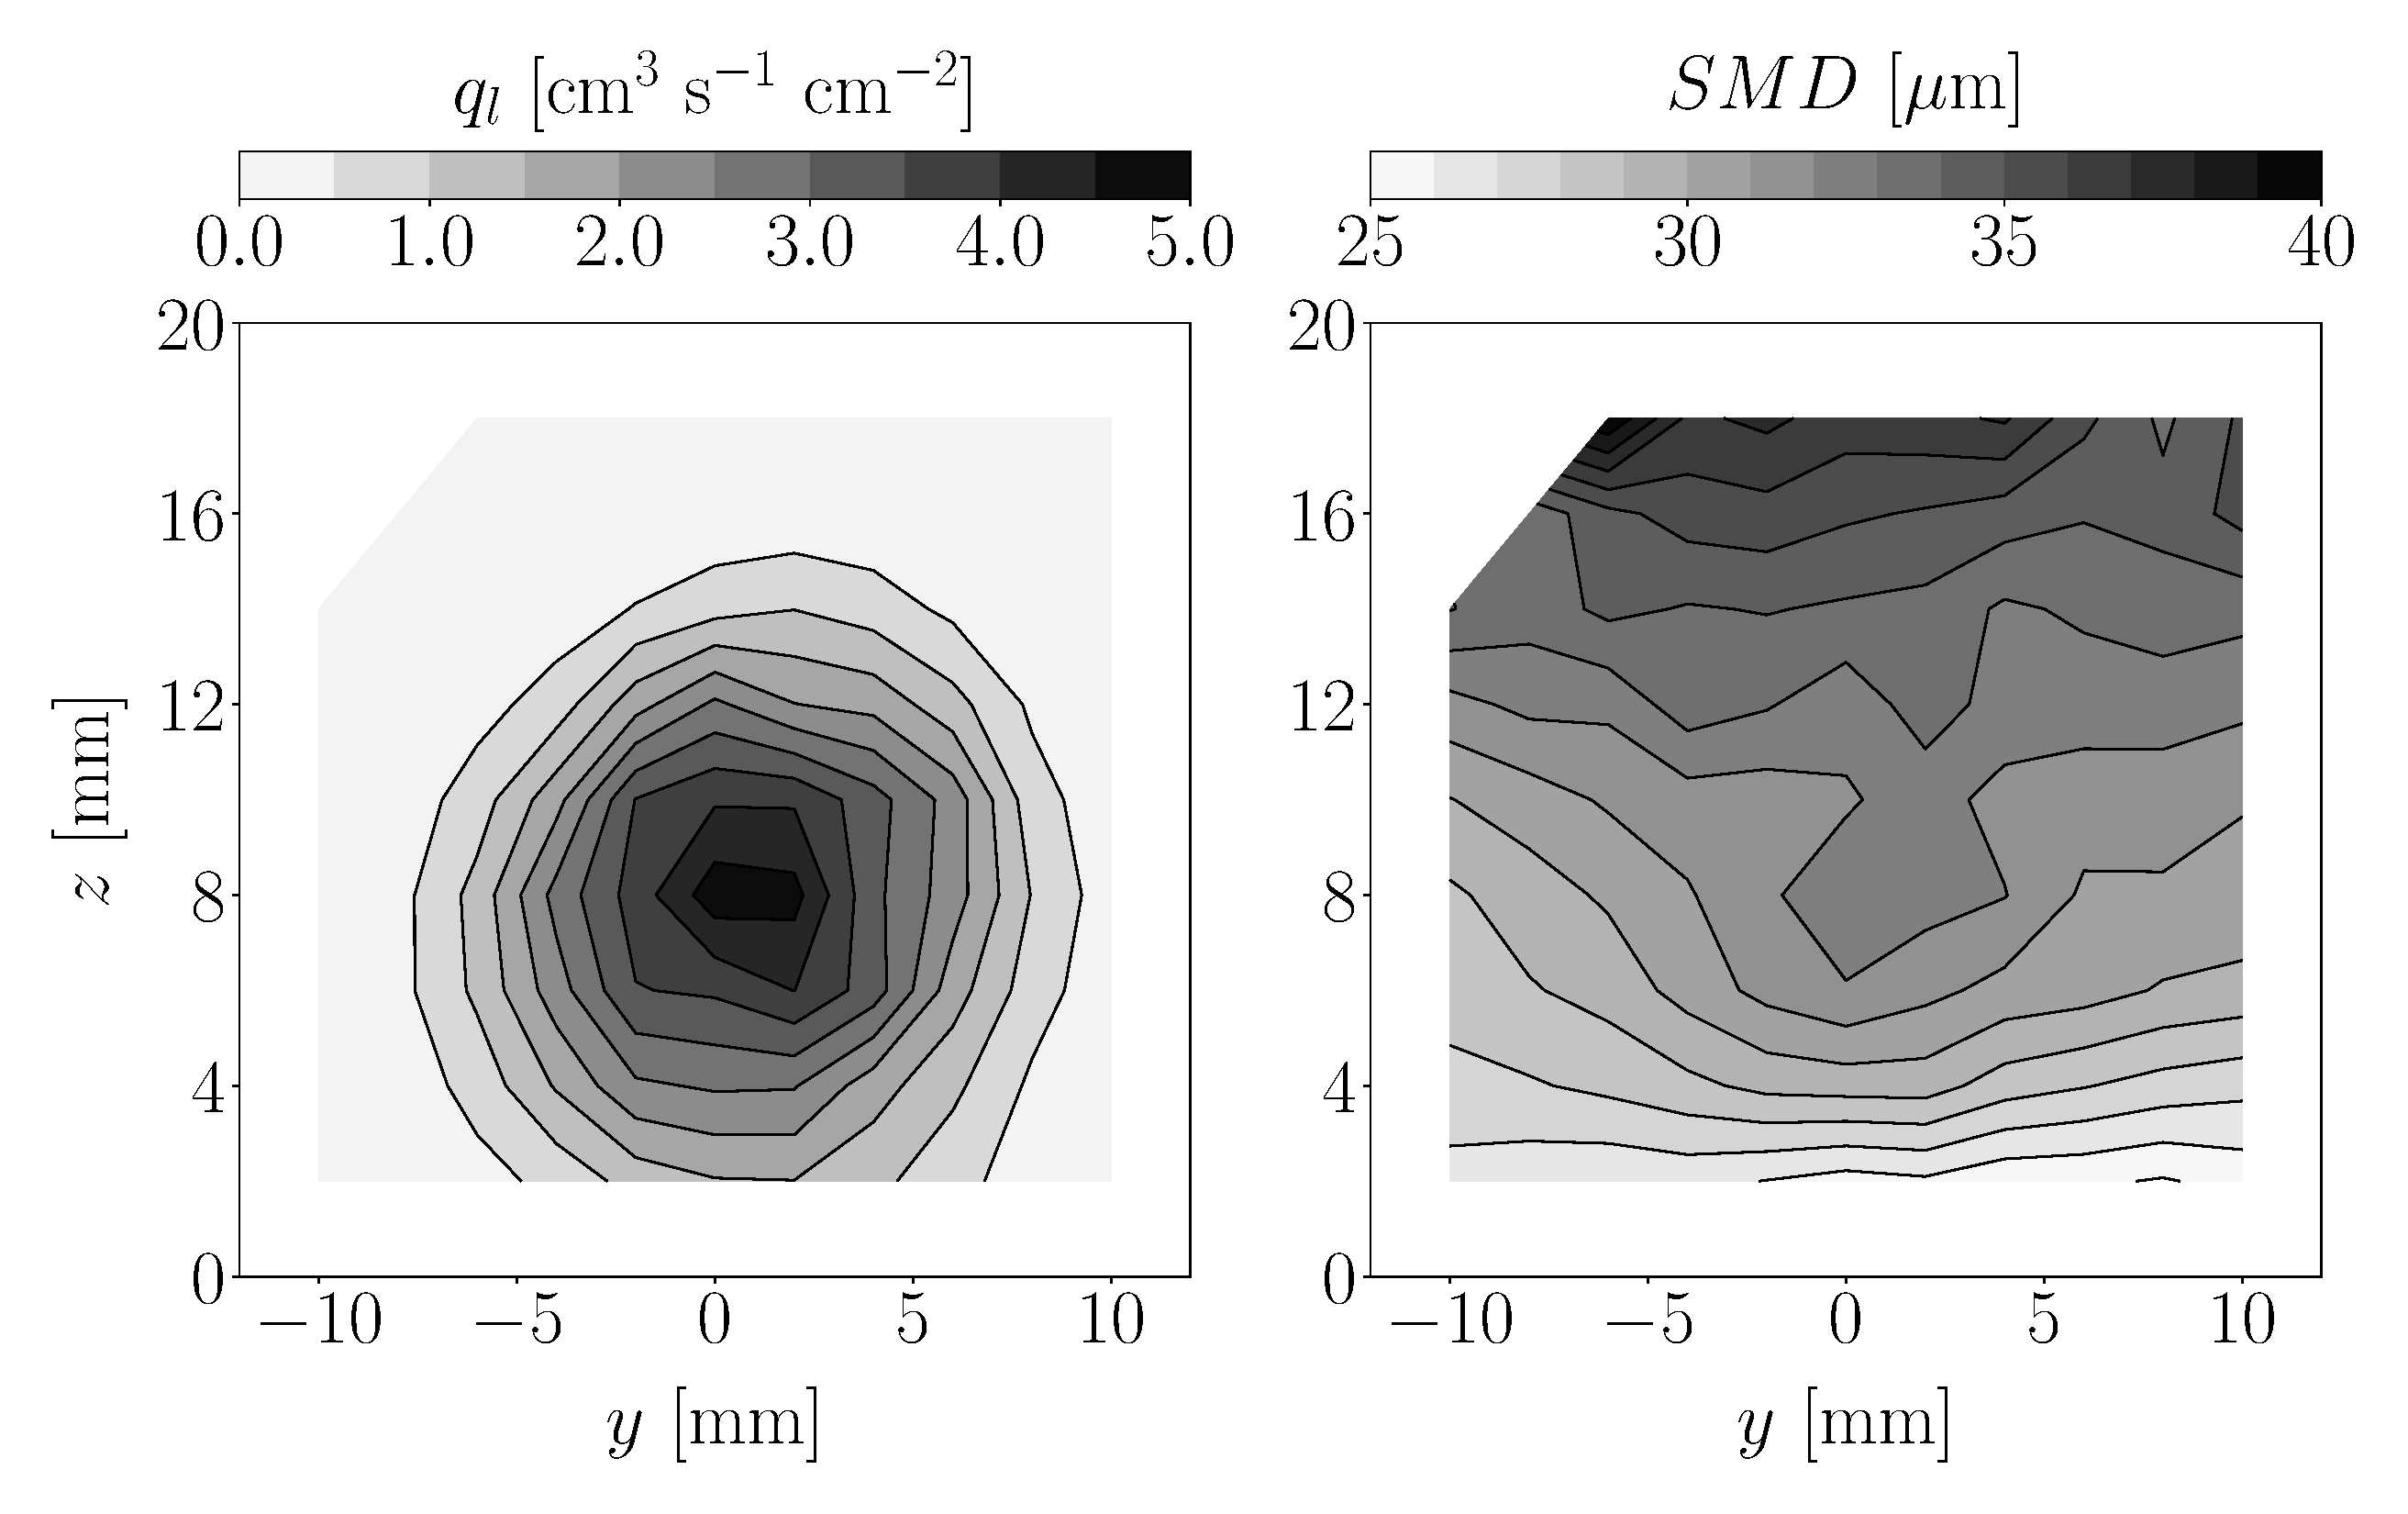
\includegraphics[scale=0.19]{./part2_developments/figures_ch6_lagrangian_JICF/expe_results/maps_UG100}
   \vspace*{-0.15in}
\caption{SMD and volume flux maps for the high Weber case obtained experimentally by \citeColor[becker_breakup_2002] at a location $x = 80$ mm downstream the liquid injector}
\label{fig:maps_Becker_expe_results}
\end{figure}

\vspace*{-0.1in}

Apart from the maps, quantitative results are also reported. These ones are given as the integrated profiles of the liquid volume flux and flux-averaged $SMD$ over the $z$ and $y$ directions, which are then respectively dependent on $y$ and $z$. The expressions used to calculate such measurements are given by Eqs. (\ref{eq:integrated_results_Becker_expe_results}):

\vspace*{-0.1in}

\begin{subequations}
\label{eq:integrated_results_Becker_expe_results}
\begin{align}
\langle q_l \rangle \left( z \right)  = \frac{1}{L_y} \int_0^{L_y} q_l \left( y, z \right) dy    & ~~~~  ; & \langle SMD \rangle \left( z \right) = \frac{1}{L_y \langle q_l \left( z \right) \rangle} \int_0^{L_y} q_l \left( y, z \right) SMD \left( y, z \right) dy \\
\langle q_l  \rangle \left( y \right) = \frac{1}{L_z} \int_0^{L_z} q_l \left( y, z \right) dz    & ~~~~  ; & \langle SMD \rangle  \left( y \right)  =  \frac{1}{L_z \langle q_l \left( z \right) \rangle} \int_0^{L_z} q_l \left( y, z \right) SMD \left( y, z \right) dz
\end{align}
\end{subequations}



Figure \ref{fig:integrated_results_Becker_expe_results} shows the profiles obtained by applying these expressions to the experimental results. The integrated volume flux over $y$ (Figure \ref{fig:integrated_results_Becker_expe_results_over_y}) shows the maximum flux to be located at $z \sim 8$ mm. Above this location, flux decreases with $z$ until there is no more liquid present. Flux values are generally larger for the high Weber point than for the low Weber one, and liquid penetrates further in the former than in the latter due to its larger liquid velocity at injection. Regarding the SMD profiles, both cases follow a ballistic behaviour. The spray of the low Weber point contains droplets of larger mean size than the high Weber one.

With respect to the profiles integrated over $z$ (Figure \ref{fig:integrated_results_Becker_expe_results_over_z}), both SMD and flux lines follow parabollic profiles with maxima located at $y = 0$. The behaviour of the profiles depending on the operating point follow the same tendencies than in Figure \ref{fig:integrated_results_Becker_expe_results_over_y}: lower fluxes and larger droplets for the low $We$ case.



\begin{figure}[h!]
\flushleft
\begin{subfigure}[b]{0.45\textwidth}
	\flushleft
   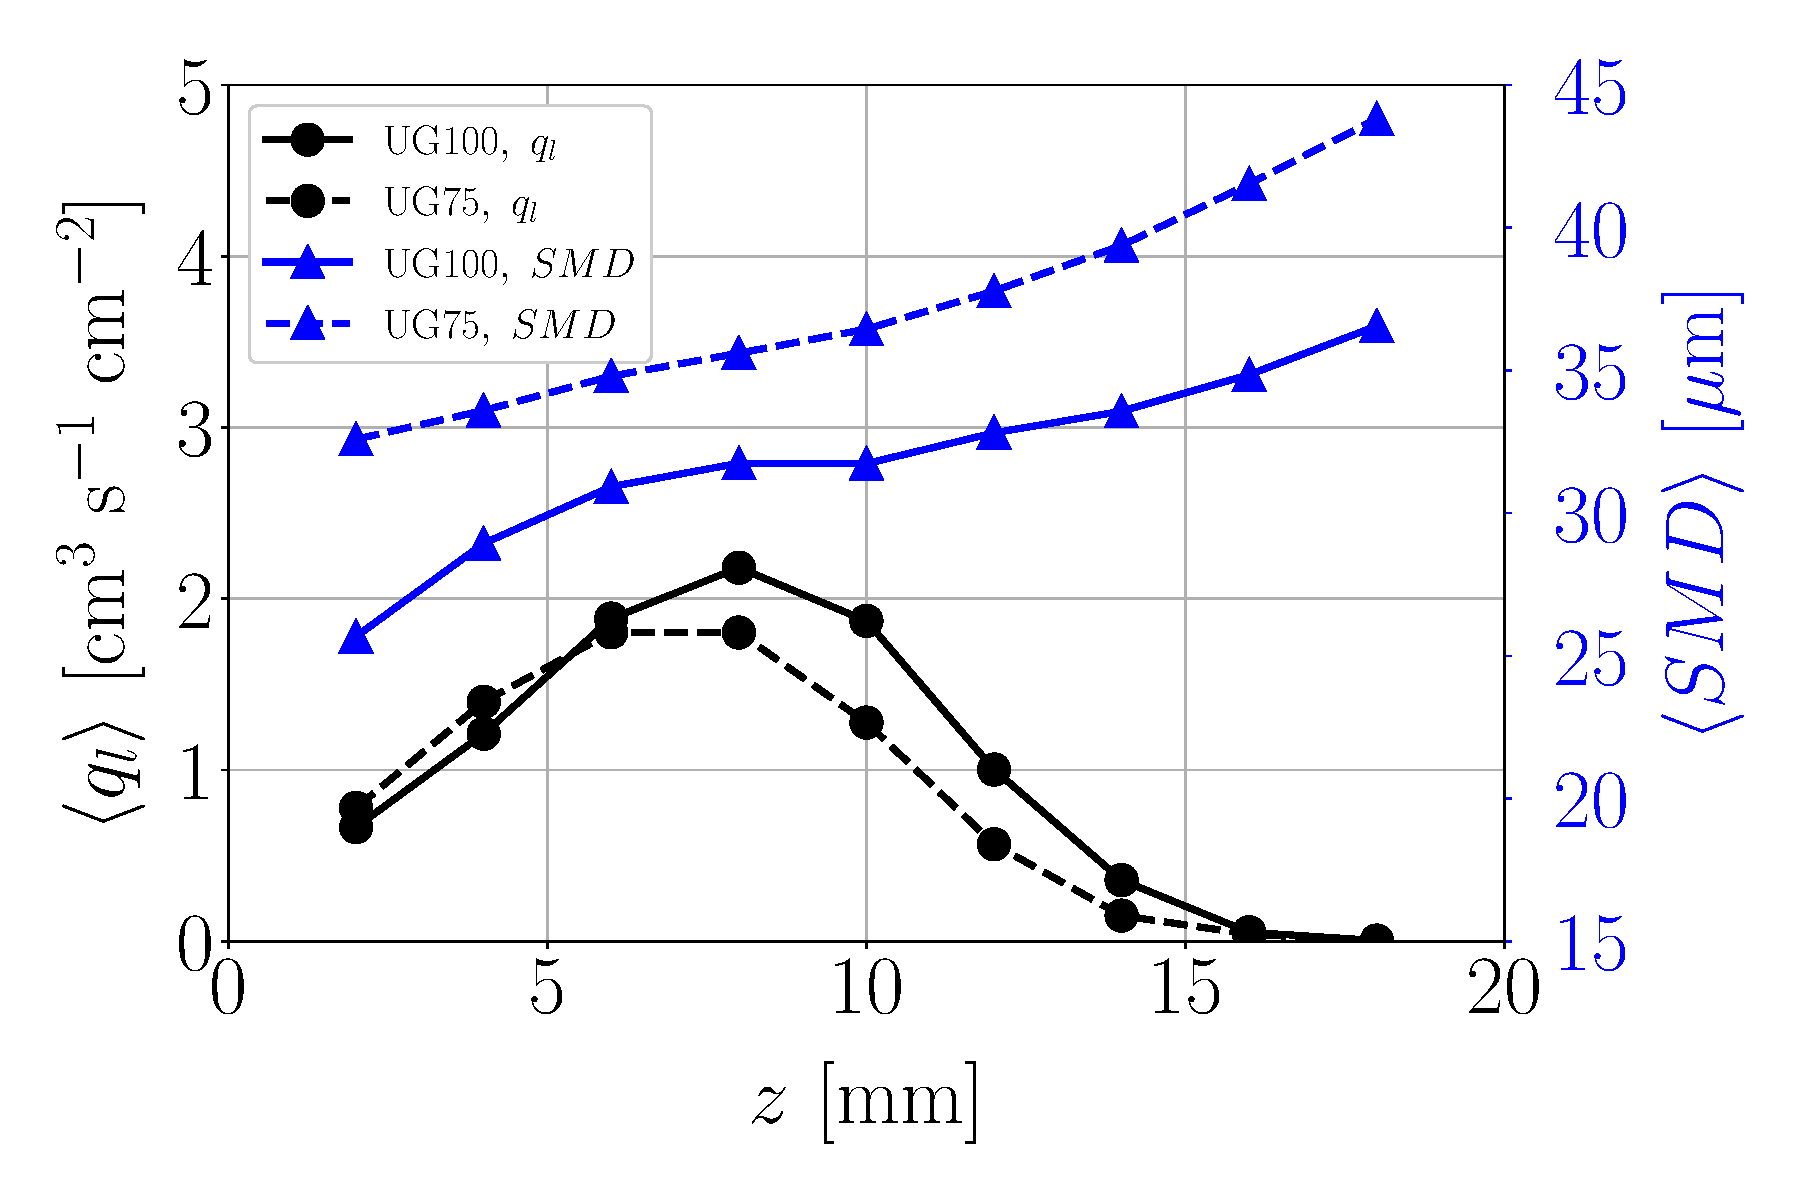
\includegraphics[scale=0.275]{./part2_developments/figures_ch6_lagrangian_JICF/expe_results/integrated_fluxes_along_y}
   \vspace*{-0.2in}
   \caption{Profiles integrated over $y$.}
  \label{fig:integrated_results_Becker_expe_results_over_y} 
\end{subfigure}
\hspace{0.3in}
\begin{subfigure}[b]{0.45\textwidth}
	\centering
   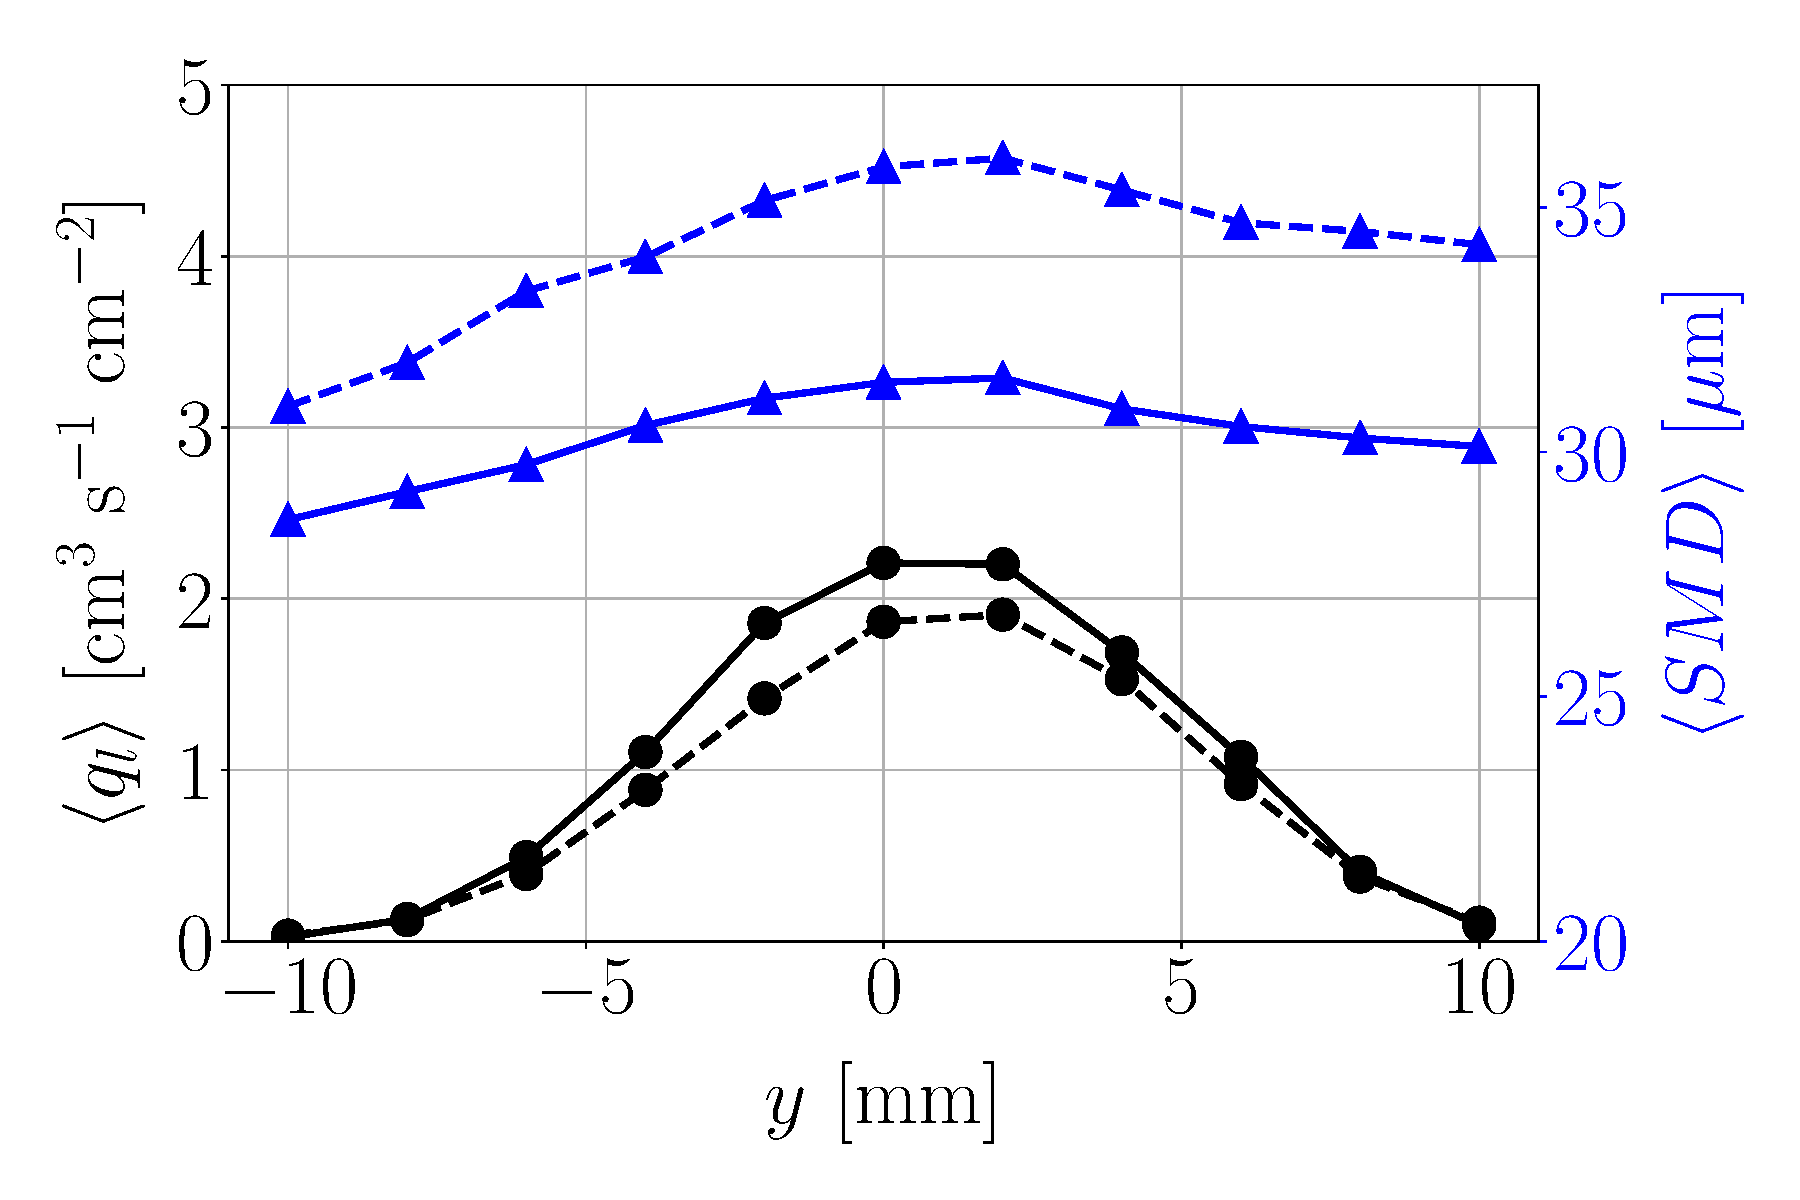
\includegraphics[scale=0.275]{./part2_developments/figures_ch6_lagrangian_JICF/expe_results/integrated_fluxes_along_z}
   \vspace*{-0.2in}
   \caption{Profiles integrated over $z$.}
  \label{fig:integrated_results_Becker_expe_results_over_z}
\end{subfigure}
\caption[{Integrated liquid volume flux and SMD profiles by \citeColor[becker_breakup_2002] at a location $x = 80$ mm downstream the liquid injector.}]{Integrated liquid volume flux and SMD profiles by \citeColor[becker_breakup_2002] at a location $x = 80$ mm downstream the liquid injector for both operaing points from Table \ref{tab:jicf_operating_conditions}}
\label{fig:integrated_results_Becker_expe_results}
\end{figure}

\clearpage

Finally, the overall SMDs estimated from PDA measurements are reported in Table \ref{tab:becker_hassa_SMD_values_sprays}.


\begin{table}[!h]
\centering
\caption{Experimental SMDs at $x = 80$ mm  }
\vspace*{-0.1in}
\begin{tabular}{cc}
\thickhline
\textbf{Operating point} & $SMD~\left[ \mu \mathrm{m}\right]$  \\
\thickhline
Low Weber & 35.2  \\  
High Weber & 31.0 \\
\thickhline
\end{tabular}
\label{tab:becker_hassa_SMD_values_sprays}
\end{table}

\vspace*{-0.3in}

\subsubsection*{Sources of uncertainty}


The experimental results previously shown were obtained through Phase Doppler Anemometry (PDA) measurements. PDA is built on the assumption that droplets are spherical, hence such measurements can therefore yield considerable errors on droplets sizes and fluxes \citepColor[tropea_optical_2011]. Several sources of error have been identified in the past. \citeColor[bachalo_method_1980] explained that the optical setup plays a paramount role, since it can lead to the misalignment of dual-beam reflected and refracted rays (Gaussian beam Effect) which can pollute the measurements. In this sense, \citeColor[doublet_effet_2019] showed through an error propagation analysis that the uncertainties in the diameters were actually especially sensitive to the elevation angle of the PDA detectors. \citeColor[damaschke_optical_1998] discussed the role of the droplet non-sphericity, stating that PDA is prone to size overestimation when particles are deformed or oscillate in a preferential direction. \citeColor[dullenkopf_comparative_1998] identified three main sources of error in fluxes estimation: 1) the particles size measurement (from which the flux is calculated, hence propagating the error), 2) the number count of droplets, and 3) the reference area used for measurements (the smaller the area the better, since it can also avoid counting droplets twice). \citeColor[brandt_experimental_1998] tested an airblast configuration and discussed several possible sources of error in sizes, highlighting the contribution of alignment uncertainties in the setup ($\sim 1~\%$), the change in refractive indices due to heating ($\sim 3.5~\%$), and the deformation of the sampled particles, which is common at high speed environments (such as the found found in airblast). They estimated a 7 $\%$ for the uncertainty on droplets sizes and a 10 $\%$ in fluxes if the concencentration of particles was not too high. It is worth mentioning that their test bench is the same one that  \citeColor[becker_breakup_2002] used later at DLR to test the liquid kerosene JICF dealt in this thesis. The experiments from \citeColor[becker_breakup_2002] do not actually provide data on the sizes uncertainties, but do discuss errors on fluxes for which they report mean deviations of 20 $\%$ and maximum of 37 $\%$. \citeColor[tropea_optical_2011] makes a review on experimental methods involving optical techniques to characterize disperse multiphase flows, and states that PDA measurements often show flux uncertainties from $20~\%$ up to several hundreds, while errors in particle size often range ideally between 10 and 30 $\%$. 

The objective here is to estimate uncertainties in the experimental measurements of \citeColor[becker_breakup_2002] to obtain confidence intervals for validation of numerical results. As mentioned in the previous paragraph, they provide a mean uncertainty of 20 $\%$ for fluxes, but do not give any information on sizes. For the same test bench but with different atomizers and operating conditions, \citeColor[brandt_experimental_1998] report errors of 7 $\%$ and 14 $\%$ for the droplets diameters and fluxes, respectively. Even though the PDA setup is identical in both studies, the provided errors in fluxes differ among each other: this might be due to different operating conditions, the atomizer or misalignments in the optical setup in both experiments. Therefore, to estimate the diameter uncertainty for the study of \citeColor[becker_breakup_2002], the relation between droplets sizes and fluxes errors is assumed to be identical as in \citeColor[brandt_experimental_1998], who state uncertaintes for fluxes to be twice larger than for sizes. Applying this factor to  \citeColor[becker_breakup_2002] yields mean diameter uncertainties of 10 $\%$. It is important to keep in mind that this estimated error in droplets size is only approximative and could greatly vary in the actual experiments. \\ %Generally, as shown by the previous literature review,  errors in PDA measurements on droplets sizes are not often reported and characteristic 

Since \citeColor[becker_breakup_2002] give values on the flux uncertainties and their experimental data are available through the maps, it is possible to estimate the luxes obtained in the experiments. The flux map ax $x = 80$ mm for the high Weber operating condition is shown in Figure \ref{fig:maps_previous_numerical_results}a. The grid which was used in the experiments to sample the spray and process the data, which is composed of 2 mm sides probes, is also displayed. Each probe contains a volume flux value $q_l$ which is stored at the center of the probe to plot the maps (as done in the SLI injectors of Figures 
\ref{fig:injectors_sli_uG75_dx10_x05} to \ref{fig:injectors_sli_uG100_dx20_x10_NT}). The grid is then composed of $N_y = 11$ probes in the lateral direction and $N_z = 9$ in the vertical one. Given an arbitrary probe located at a position $\left( j,k \right)$ (where $j$ is the probe index in the lateral direction $y$ and $k$ in the vertical one $z$) with surface $S_\mathrm{j,j}$, the absolute liquid flux through this probe can be calculated by applying Eq. (\ref{eq:ch4_volume_flux_definition}) to the probe volume flux $q_{l{j,k}}$:

\begin{equation}
Q_{l_{j,k}} = q_{l_{j,k}} S_{j,k}
\end{equation}

Then, the total liquid flow rate from the map can be calcuated by adding all the absolute fluxes from each probe:

\begin{equation}
\label{eq:ch6_Ql_total_estimation_from_flux_profiles}
Q_{l} = \sum_{j=1}^{N_y} \sum_{k=1}^{N_z} Q_{l_{j,k}} = \sum_{j=1}^{N_y} \sum_{k=1}^{N_z} q_{l_{j,k}} S_{j,k} = 4062 ~ \mathrm{mm}^3~\mathrm{s}^{-1}
\end{equation}

which, as shown, gives a value of $4062 ~ \mathrm{mm}^3~\mathrm{s}^{-1}$. The injected flow rate for this case is $Q_{l,\mathrm{inj}} = 3710~ \mathrm{mm}^3~\mathrm{s}^{-1}$, as given in Table \ref{tab:jicf_operating_conditions}. Therefore, the PDA measurements report a flux excess of $9.5~\%$ with respect to the injected flow rate. This deviation is comprised within the mean uncertainty of $20~\%$ provided by the authors of the experiments. Nevertheless, it is paramount to consider this flux overestimation when comparing to dispersed-phase simulations, since liquid is injected with SLI in these ones at a rate of  $Q_{l,\mathrm{inj}} = 3710~ \mathrm{mm}^3~\mathrm{s}^{-1}$. In reality, if the PDA was exempt of errors, the retrieved experimental flux could not be larger than the injected one (mass is not created in the simulation). Indeed, it should be lower since there is filming in the experiments, as shown in Figure \ref{fig:jicf_snapshot_expe_filming}, that reduces the liquid flux perpendicular to the crossflow. The resolved simulations could capture this filming phenomenon in the jet.

\begin{figure}[h!]	
	\centering	
	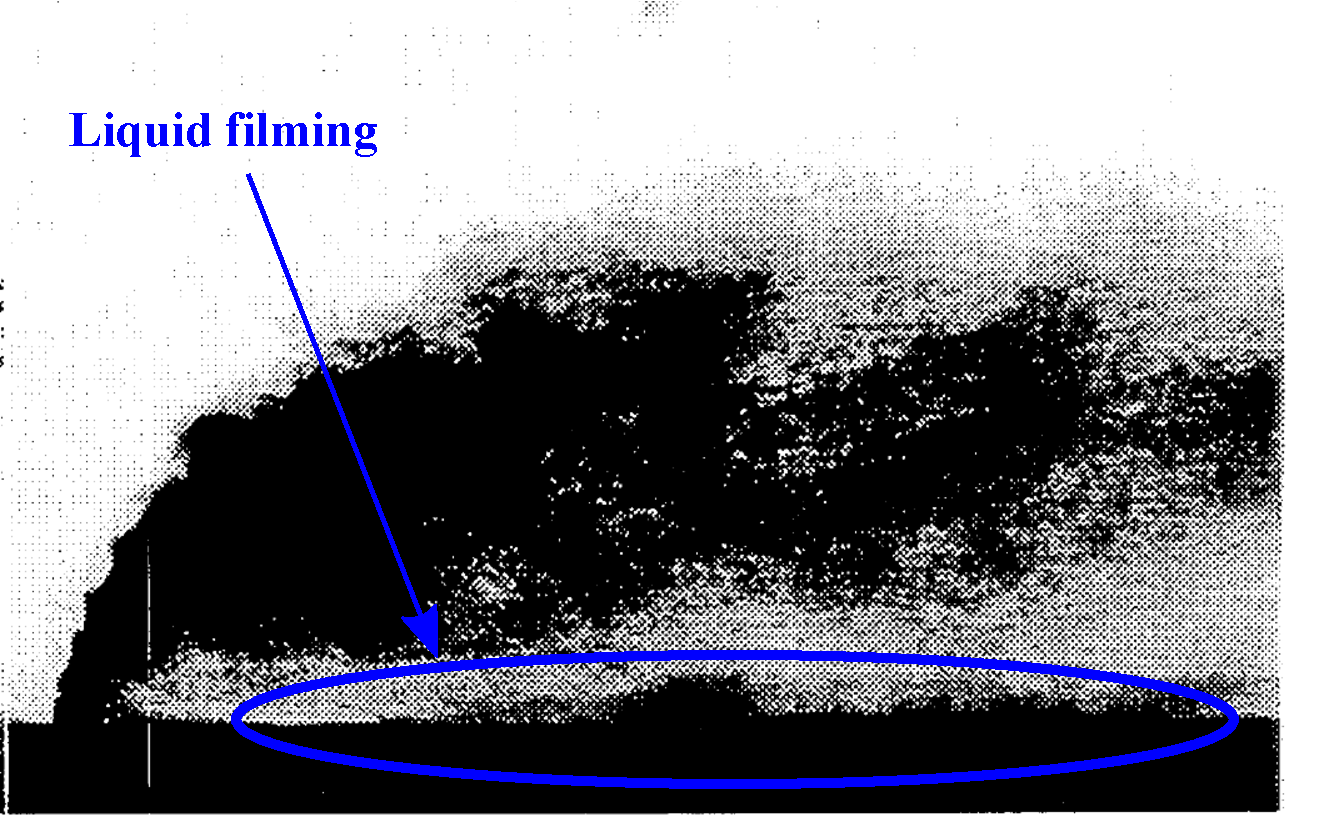
\includegraphics[scale=0.4]{./part2_developments/figures_ch6_lagrangian_JICF/expe_results/snapshot_expe_filming}
	\caption{Snapshot of instantaneous liquid jet from \citeColor[becker_breakup_2002], showing the filming phenomenon}
	\label{fig:jicf_snapshot_expe_filming}
\end{figure}




\subsection{Previous numerical studies}
\label{ch6:previous_numerical_studies}

The experimental configuration of \citeColor[becker_breakup_2002] has been studied through computations by several authors, all of them simulating the high Weber operating point from Table \ref{tab:jicf_operating_conditions}. \citeColor[rachner_modelling_2002] simulated the jet in steady crossflow by considering the early liquid as a cylinder deflected by the airflow, which exchanges momentum with a modified drag coefficient, sheds mass and produces droplets whose properties are given from experimental correlations. Later on, \citeColor[eckel_semi-empirical_2016] extended this model to account for shear breakup of ellipsoids and flattened liquid jets (to account for more realistic JICF dense core effects) in both steady and unsteady crossflows, by using semi-empirical correlations. Independently of these studies, \citeColor[jaegle_large_2009] and \citeColor[senoner_simulation_2010] also developed models with this configuration: the former injected a developed spray at the liquid nozzle while accounting for a modified drag law in the near-nozzle region to mimic the liquid column momentum exchange, and the later injected big blobs at the nozzle but accounting for secondary atomization. All these models (except for
\citeColor[rachner_modelling_2002] since it was more recently improved by \citeColor[eckel_semi-empirical_2016]) are summarized in the diagram of Figure \ref{ch3:subsec_lagrangian_liquid_JICF} and detailed in $\S$\ref{fig:state_art_injection}.

In order to position the current work into the state of the art, it is worth to compare it to the previous studies performed. All the works aforementioned use data shown in Figure \ref{fig:maps_Becker_expe_results} to validate the computations. Nevertheless, not all the numerical studies previously mentioned use all these data for validation, but only display a few of them. Table \ref{tab:previous_numerical_studies_on_jicf_dlr_recap} shows a summary of the validation data directly available in the previous works. None of the papers referred present data on the SMD map, while only \citeColor[eckel_semi-empirical_2016] give data on the global SMD obtained. Most of the works give data on the flux and SMD profiles integrated over $y$, while only \citeColor[rachner_modelling_2002] provides profiles integrated over $y$. %The only work which does not provide data on SMD distributions is \citeColor[eckel_semi-empirical_2016]. 

In first place, the flux maps from all the previous works that provide these information are shown in Figure \ref{fig:maps_previous_numerical_results}. The experimental map is also show for visual comparison. In general, all maps show a circular flux shape and an overestimation of the maximum flux location in the vertical direction (the integrated maps discussed in the following lines confirm this observation). Since the data belonging to the the maps of the numerical studies were unfortunately not directly available, it was obtained by digitalizing the 2D maps depicted in the papers. The grid used for digitalizion is not shown since it was finer than the experimental grid in order to properly capture all the features of the maps, and showing it together with the maps hinders their visualization. From the digitalized maps, the total flux in the plane can be calculated as done previously for the experimental data applying Eq. (\ref{eq:ch6_Ql_total_estimation_from_flux_profiles}). The results are shown in Table \ref{tab:previous_numerical_studies_on_jicf_dlr_values}: even though the fluxes are not exactly equal to the injected flux (the digitalization methodology is not robust enough to retrieve accurately the actual fluxes plotted by the authors, which should be equal to the injected flux and therefore differ from the values obtained), all values are lower than the flux integrated from the experimental map. The only exception is \citeColor[rachner_modelling_2002]: in fact, this work does not display neither maps nor absolute rates, but normalized integrated profiles which in this case have been de-normalized with the injected flux (it has been assumed that the flux retrieved at 80 mm is equal to the injected one). The integrated profiles of the fluxes shown in Figure \ref{fig:previous_works_profiles_comparison_with_expe} confirm these lower flow rates obtained in all simulations performed by each author. These integrated profiles have been obtained through either direct digitalization of the curves when available (Table \ref{tab:previous_numerical_studies_on_jicf_dlr_recap}) or by applying Eq. (\ref{eq:integrated_results_Becker_expe_results}) to the maps when not available. The error bars in the experimental flux profiles of Figure \ref{fig:previous_works_profiles_comparison_with_expe} correspond to a deviation of 20 $\%$ in each point. 


\begin{table}[!h]
\centering
\caption{Available data from previous numerical studies on experimental validation in the configuration of  \citeColor[becker_breakup_2002]}
\begin{tabular}{cccccccc}
\thickhline
\multirow{2}{*}{ Work }  & Global & SMD & Flux & \multirow{2}{*}{ $\langle SMD \left( z \right) \rangle$} & \multirow{2}{*}{ $\langle q_l \left( z \right) \rangle$} & \multirow{2}{*}{ $\langle SMD \left( y \right) \rangle$} & \multirow{2}{*}{ $\langle q_l \left( y \right) \rangle$} \\ 
 & SMD & map & map & & & & \\ 
\thickhline
\citeColor[rachner_modelling_2002] &  & & & \checkmark & \checkmark & \checkmark & \checkmark \\
\citeColor[jaegle_large_2009] & & & \checkmark & \checkmark & \checkmark & & \\
\citeColor[senoner_simulation_2010] & & & \checkmark & \checkmark & \checkmark & & \\
\citeColor[eckel_semi-empirical_2016] & \checkmark & & \checkmark & & & & \\
\thickhline
\end{tabular}
\label{tab:previous_numerical_studies_on_jicf_dlr_recap}
\end{table}

\begin{figure}[h!]
\flushleft
\begin{subfigure}[b]{0.2\textwidth}
	\flushleft
%	\hspace*{-0.35in}
   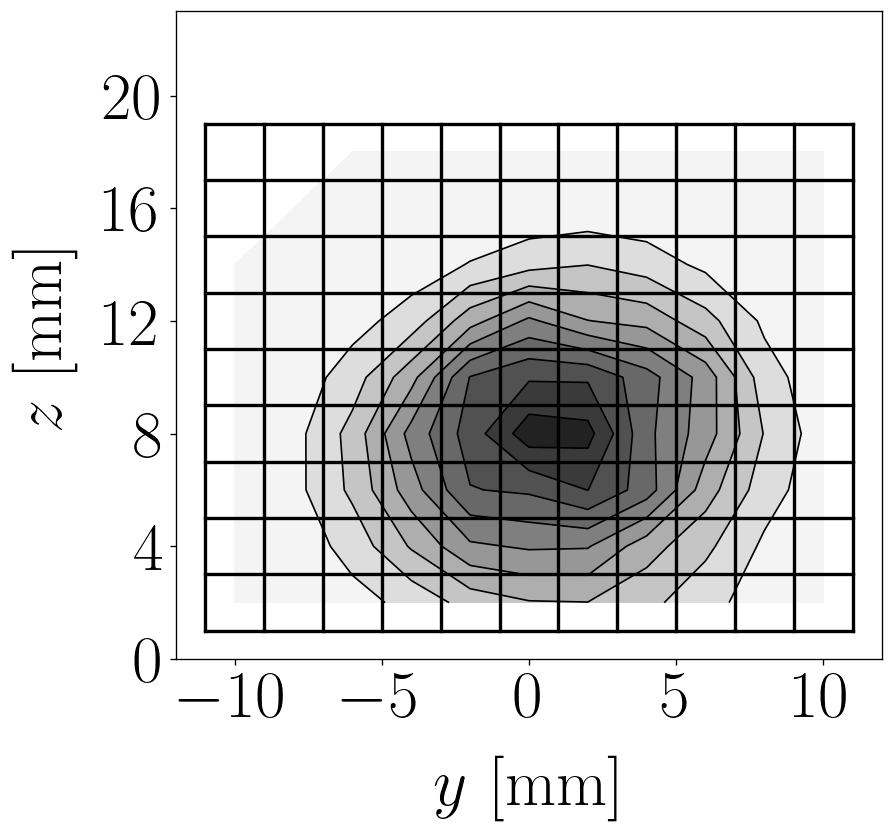
\includegraphics[scale=0.225]{./part2_developments/figures_ch6_lagrangian_JICF/previous_numerical_results/map_expe}
   \caption*{\hspace{0.35in}(a) Experimental}
   %\label{} 
\end{subfigure}
\hspace*{0.35in}
\begin{subfigure}[b]{0.2\textwidth}
	\flushleft
   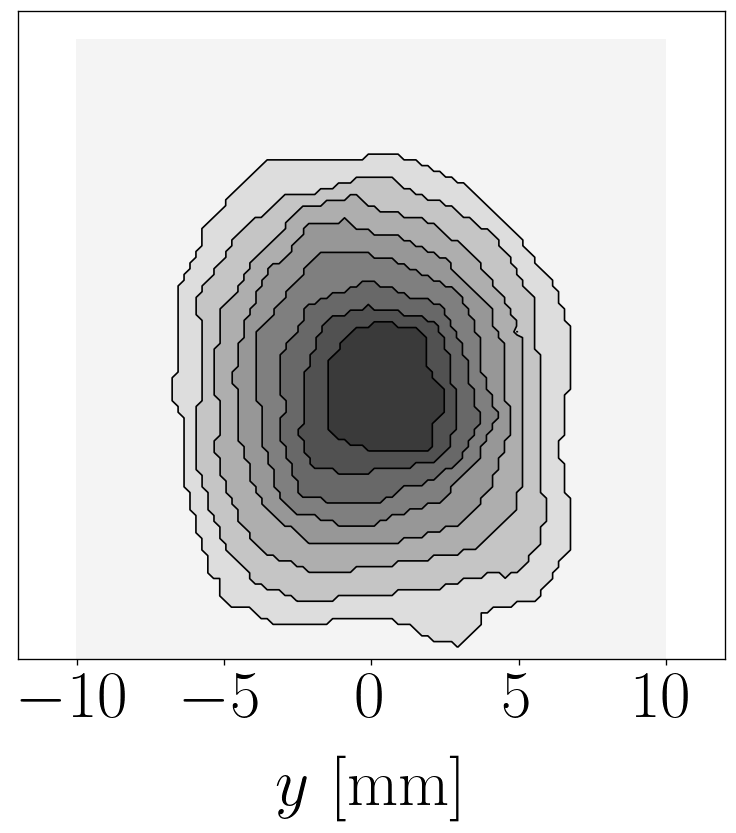
\includegraphics[scale=0.225]{./part2_developments/figures_ch6_lagrangian_JICF/previous_numerical_results/map_jaegle}
   \caption*{(b) Jaegle (2009)}
   %\label{} 
\end{subfigure}
\hspace*{0.05in}
\begin{subfigure}[b]{0.2\textwidth}
	\flushleft
   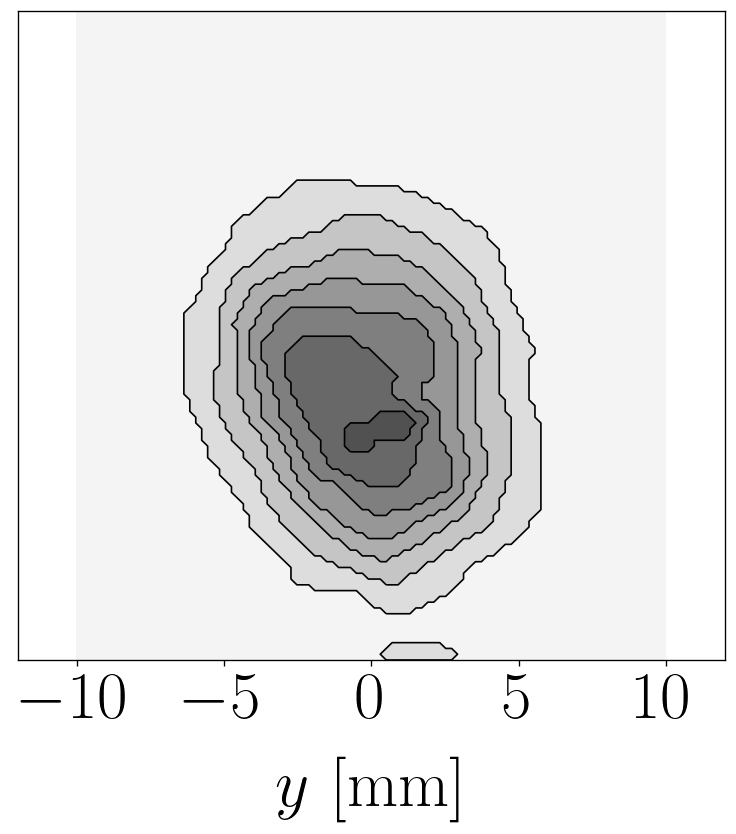
\includegraphics[scale=0.225]{./part2_developments/figures_ch6_lagrangian_JICF/previous_numerical_results/map_senoner}
   \caption*{(c) Senoner (2010)}
   %\label{} 
\end{subfigure}
\hspace*{0.05in}
\begin{subfigure}[b]{0.2\textwidth}
	\flushleft
   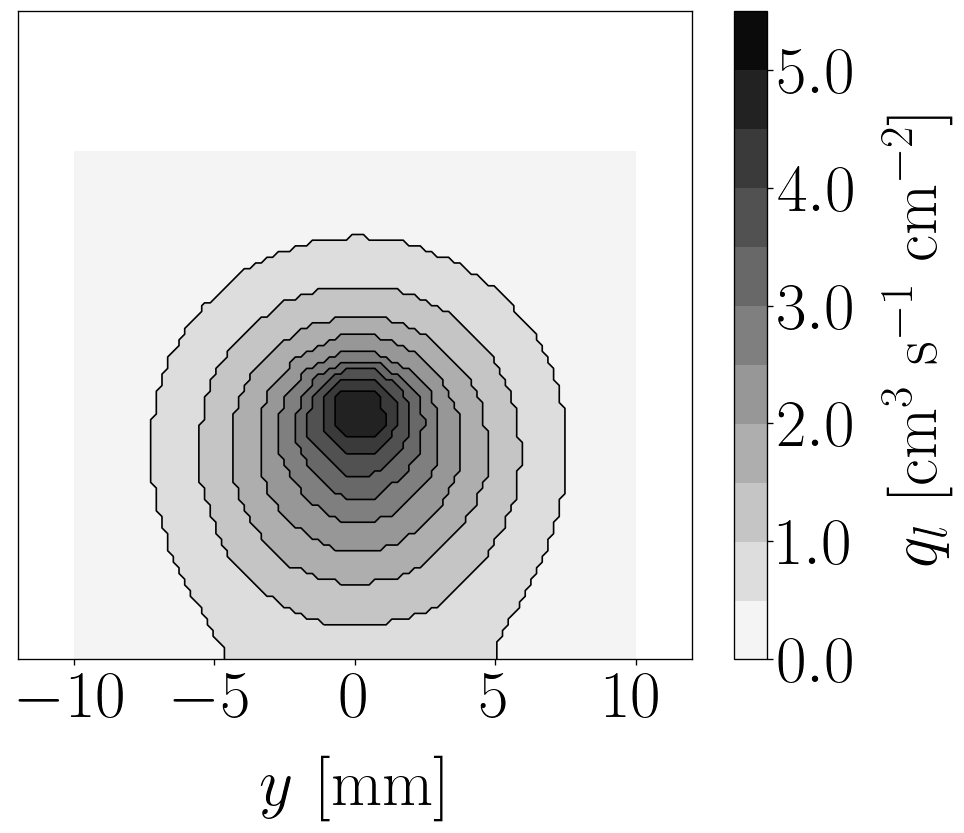
\includegraphics[scale=0.225]{./part2_developments/figures_ch6_lagrangian_JICF/previous_numerical_results/map_eckel}
   \caption*{(c) Eckel (2016)}
   %\label{} 
\end{subfigure}
\caption{Volume flux maps at $x = 80$ mm obtained for the high Weber operating conditions from experiments \citepColor[becker_breakup_2002] and past computational works on the same configuration and operating condition. The experimental map shows the grid composed of the probes through which the spray is characterized}
\label{fig:maps_previous_numerical_results}
\end{figure}

As previously mentioned, none of the previous works display SMD maps. Most of the works report, on the other hand, $SMD$ integrated profiles over $y$: these have been digitalized and are shown in Figure \ref{fig:previous_works_profiles_comparison_with_expe}.   The error bars in the experimental SMD profiles at this Figure correspond to a deviation of 10 $\%$ in each point. Furthermore, results from one computation performed with Smart Lagrangian Injectors (SLI) in this thesis are also included for comparison. All cases show a ballistic behaviour in which the SMD increases with vertical distance $z$. The SMD profiles integrate over $z$ are only present in the present work and in \citeColor[rachner_modelling_2002], who obtained accurate results at the center of the spray (region of maximum flux location) and showed a SMD overestimation when moving away towards the edges. The actual results from this thesis show that fluxes values  and the vertical location of maximum flux can be properly estimated by SLI. On the other hand, SMDs are always underestimated by SLI with respect to both experiments and computations. As it will be shown later in this chapter, this underestimation is due to secondary atomization which breaks droplets very quickly after they are injected into the liquid channel.

From the SMD integrated profiles over $y$, a global SMD can be estimated by performing a further integration along the $z$ direction:

\begin{equation}
 SMD =  \frac{1}{ \int_0^{L_z} \langle q_l \left( z \right) \rangle dz} \int_0^{L_z} \langle q_l \left( z \right) \rangle \langle SMD \left( z \right) \rangle dz
\end{equation}


Results are shown in Table \ref{tab:previous_numerical_studies_on_jicf_dlr_values}.  \citeColor[eckel_semi-empirical_2016] do not provide the integrated SMD profile, yet they give directly the global SMD. Generally, all SMDs show a good agreement with respect to the experimental value of \citeColor[becker_breakup_2002]. The works of \citeColor[rachner_modelling_2002] and \citeColor[eckel_semi-empirical_2016] perform a calibration of their model to match the experimental size distribution, hence such a good agreement is expected. Similar is the case of \citeColor[jaegle_large_2009], who already injected the experimental size distribution at the injector without including any secondary atomization model: then, the flux-weighted SMD is expected to be close to the SMD of this distribution. \citeColor[senoner_simulation_2010] does not inject any distribution but injects droplets at the liquid nozzle with size equal to the nozzle's diameter, drags them with a modified momentum transfer law at the column liquid region and then applies the stochastic secondary breakup model of \citeColor[gorokhovski_stochastic_2001], used in this thesis and explained in $\S$\ref{subsec:ch4_goro_model}, to account for further breakup of droplets. The good results in terms of global SMD and integrated profiles obtained in his work denote the suitability of the stochastic breakup model to simulate such configurations.



%\citeColor[rachner_modelling_2002], who performed the first computations on this experimental bench, stated that the injected fuel flow rate is not conserved in the measurements at $x = 80$ mm since "\textsl{PDA measurements are less accurate at high local liquid fluxes because of dense spray effects} (sic)". \hl{...} The experimental volume flux map at $x = 80$ together with the grid in whose center the measurement probes have been located is shown in Figure \hl{\textbf{XX}} left. For each discrete probe ($j,k$), the absolute flux $Q_{l_{j,k}}$ can be calculated as:


\begin{figure}[h!]
\flushleft
\begin{subfigure}[b]{0.9\textwidth}
	\centering
   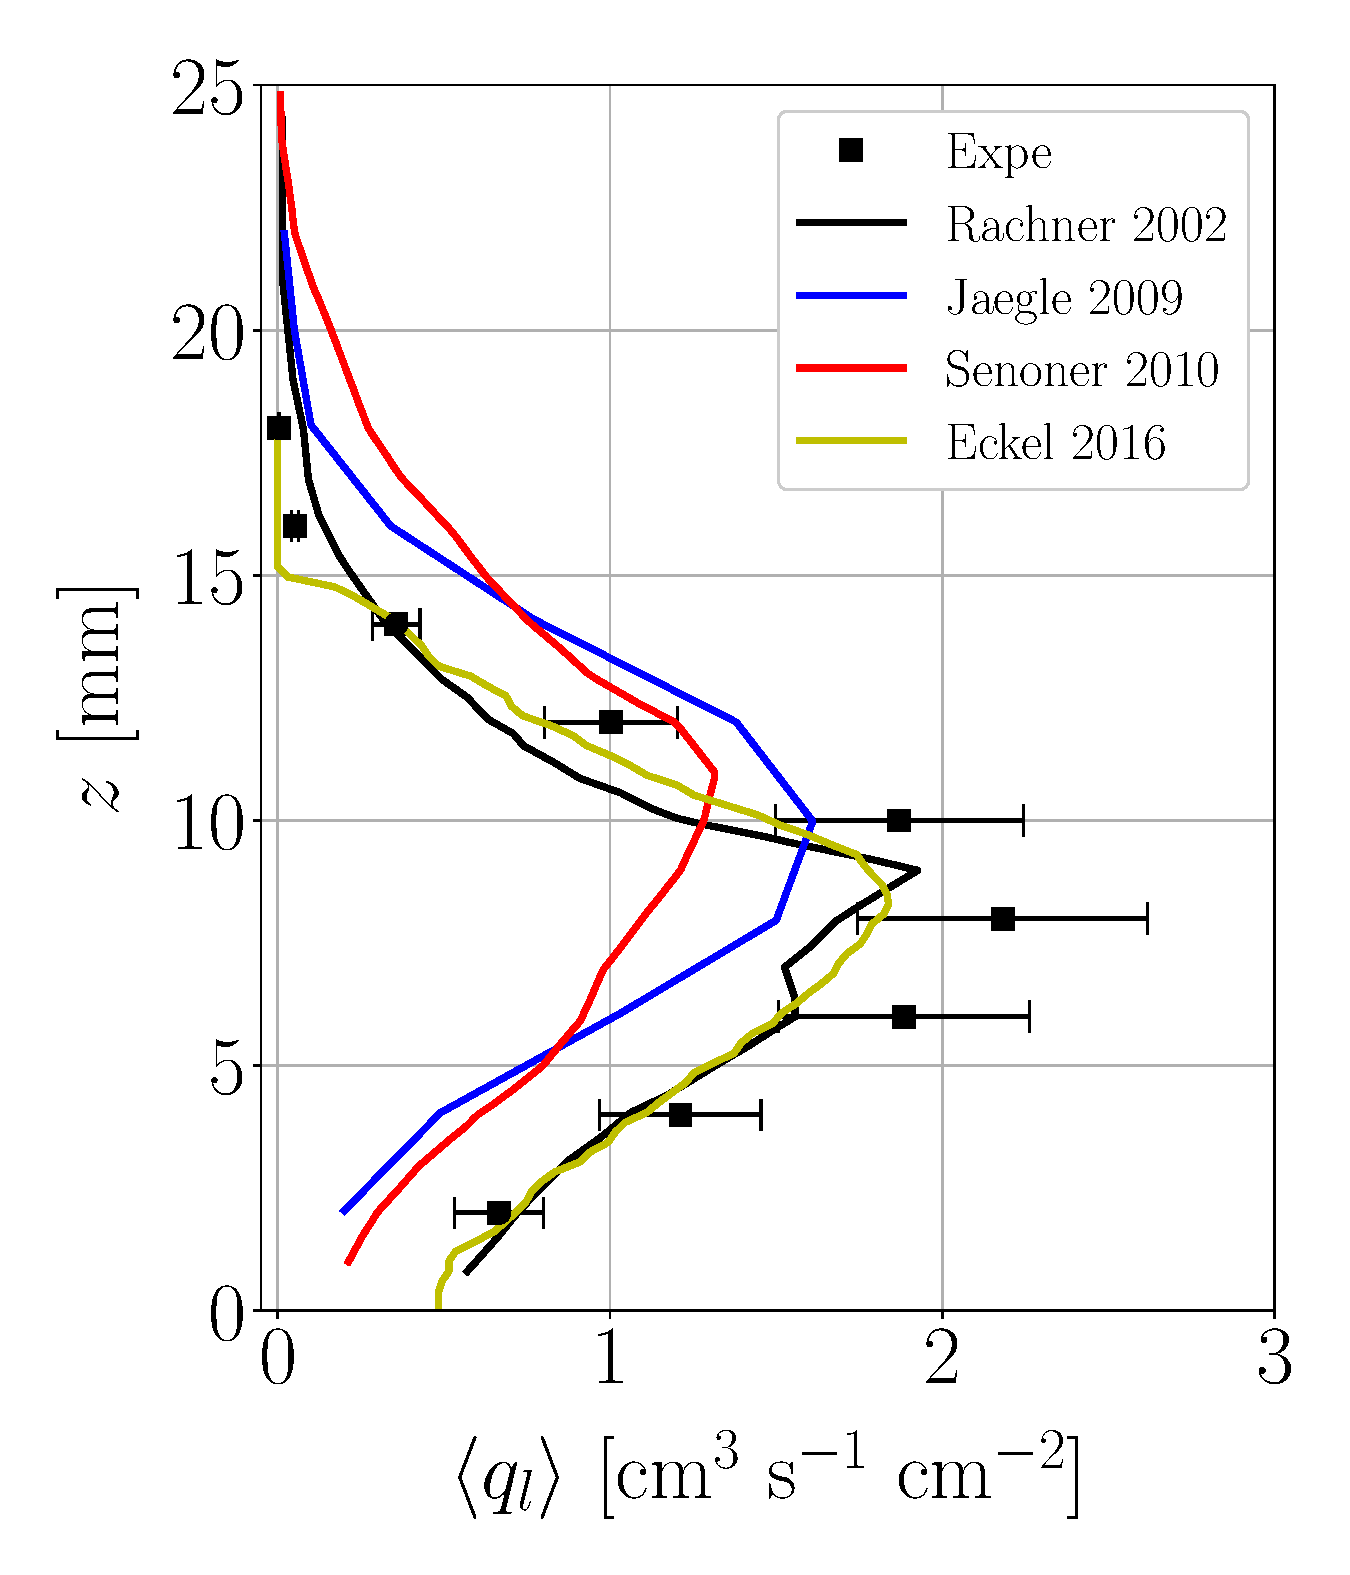
\includegraphics[scale=0.22]{./part2_developments/figures_ch6_lagrangian_JICF/previous_numerical_results/flux_profiles_along_z}
%    \hfill
   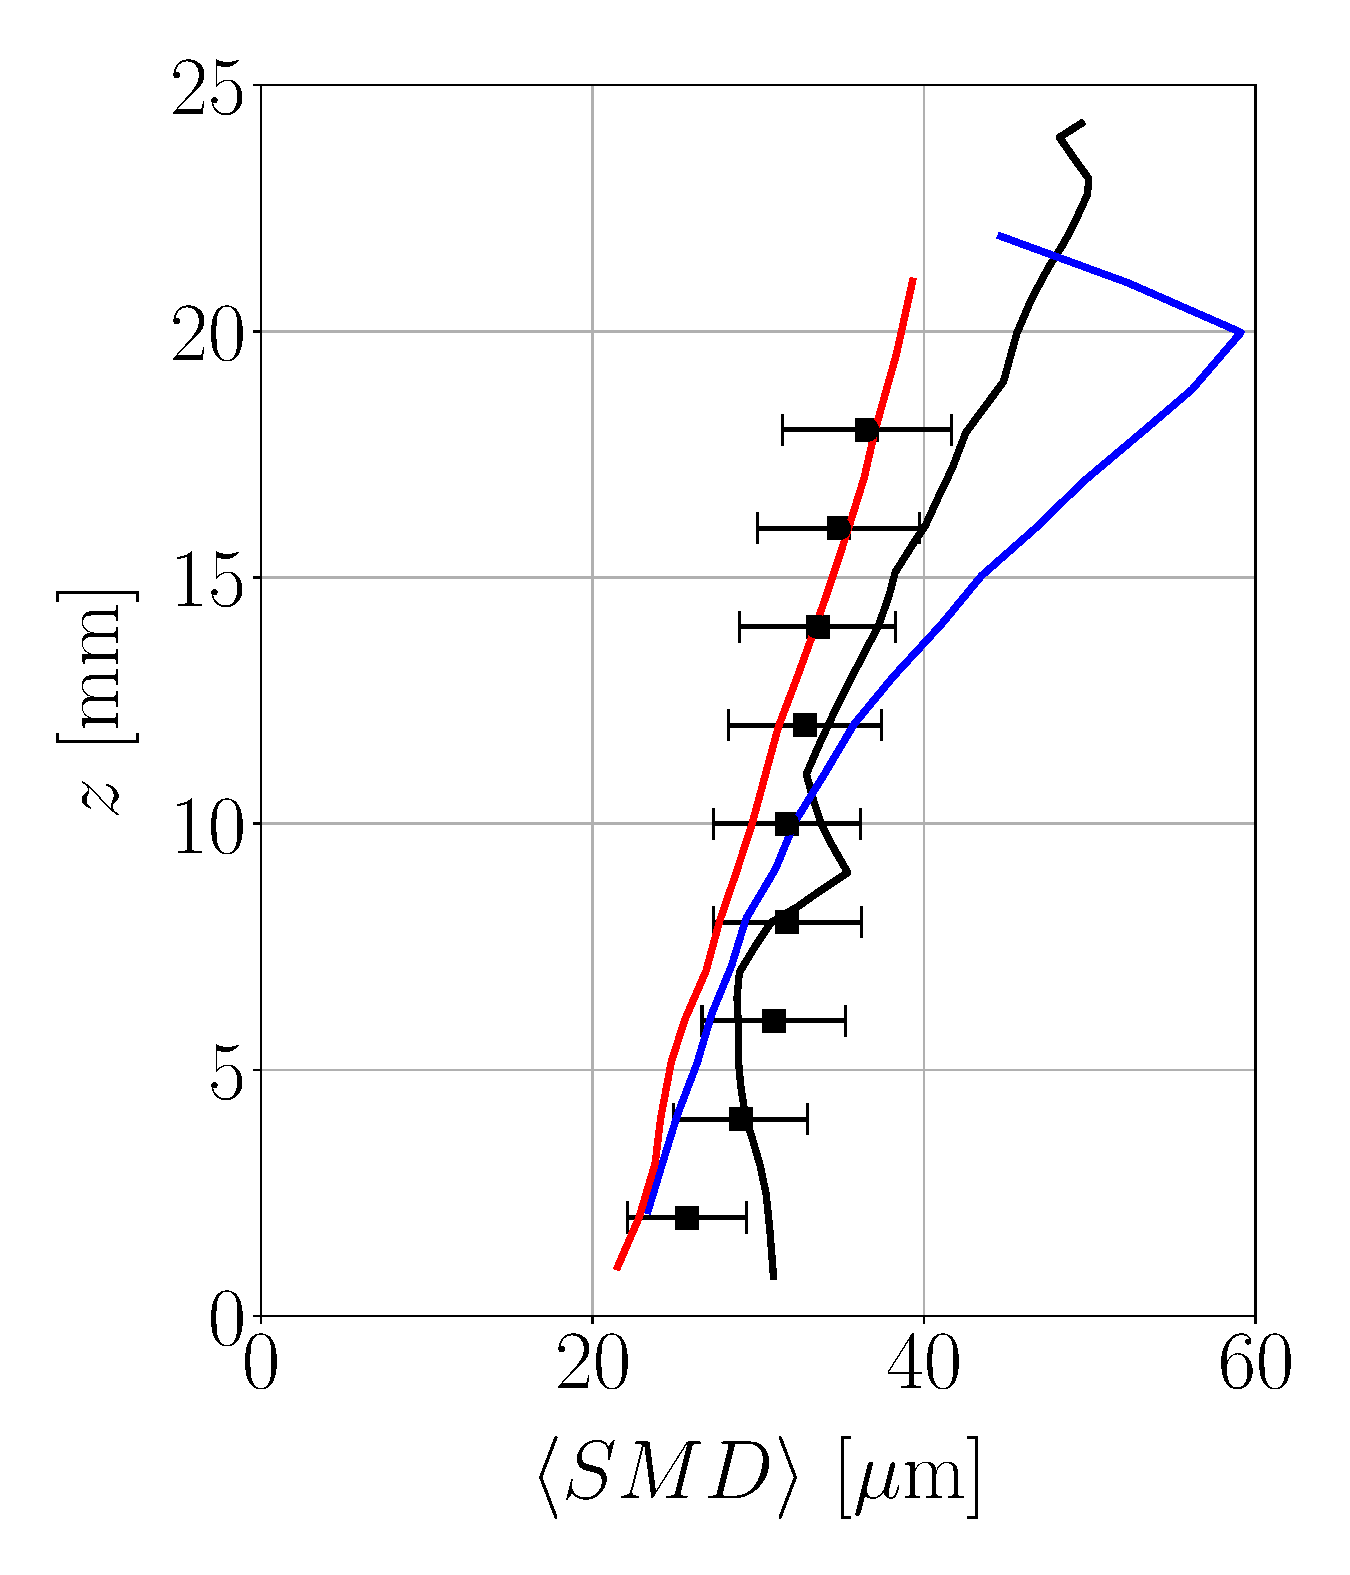
\includegraphics[scale=0.22]{./part2_developments/figures_ch6_lagrangian_JICF/previous_numerical_results/SMD_profiles_along_z}
   \caption{Profiles integrated over y}
   %\label{} 
\end{subfigure}

\vskip\baselineskip

\begin{subfigure}[b]{0.9\textwidth}
	\centering
   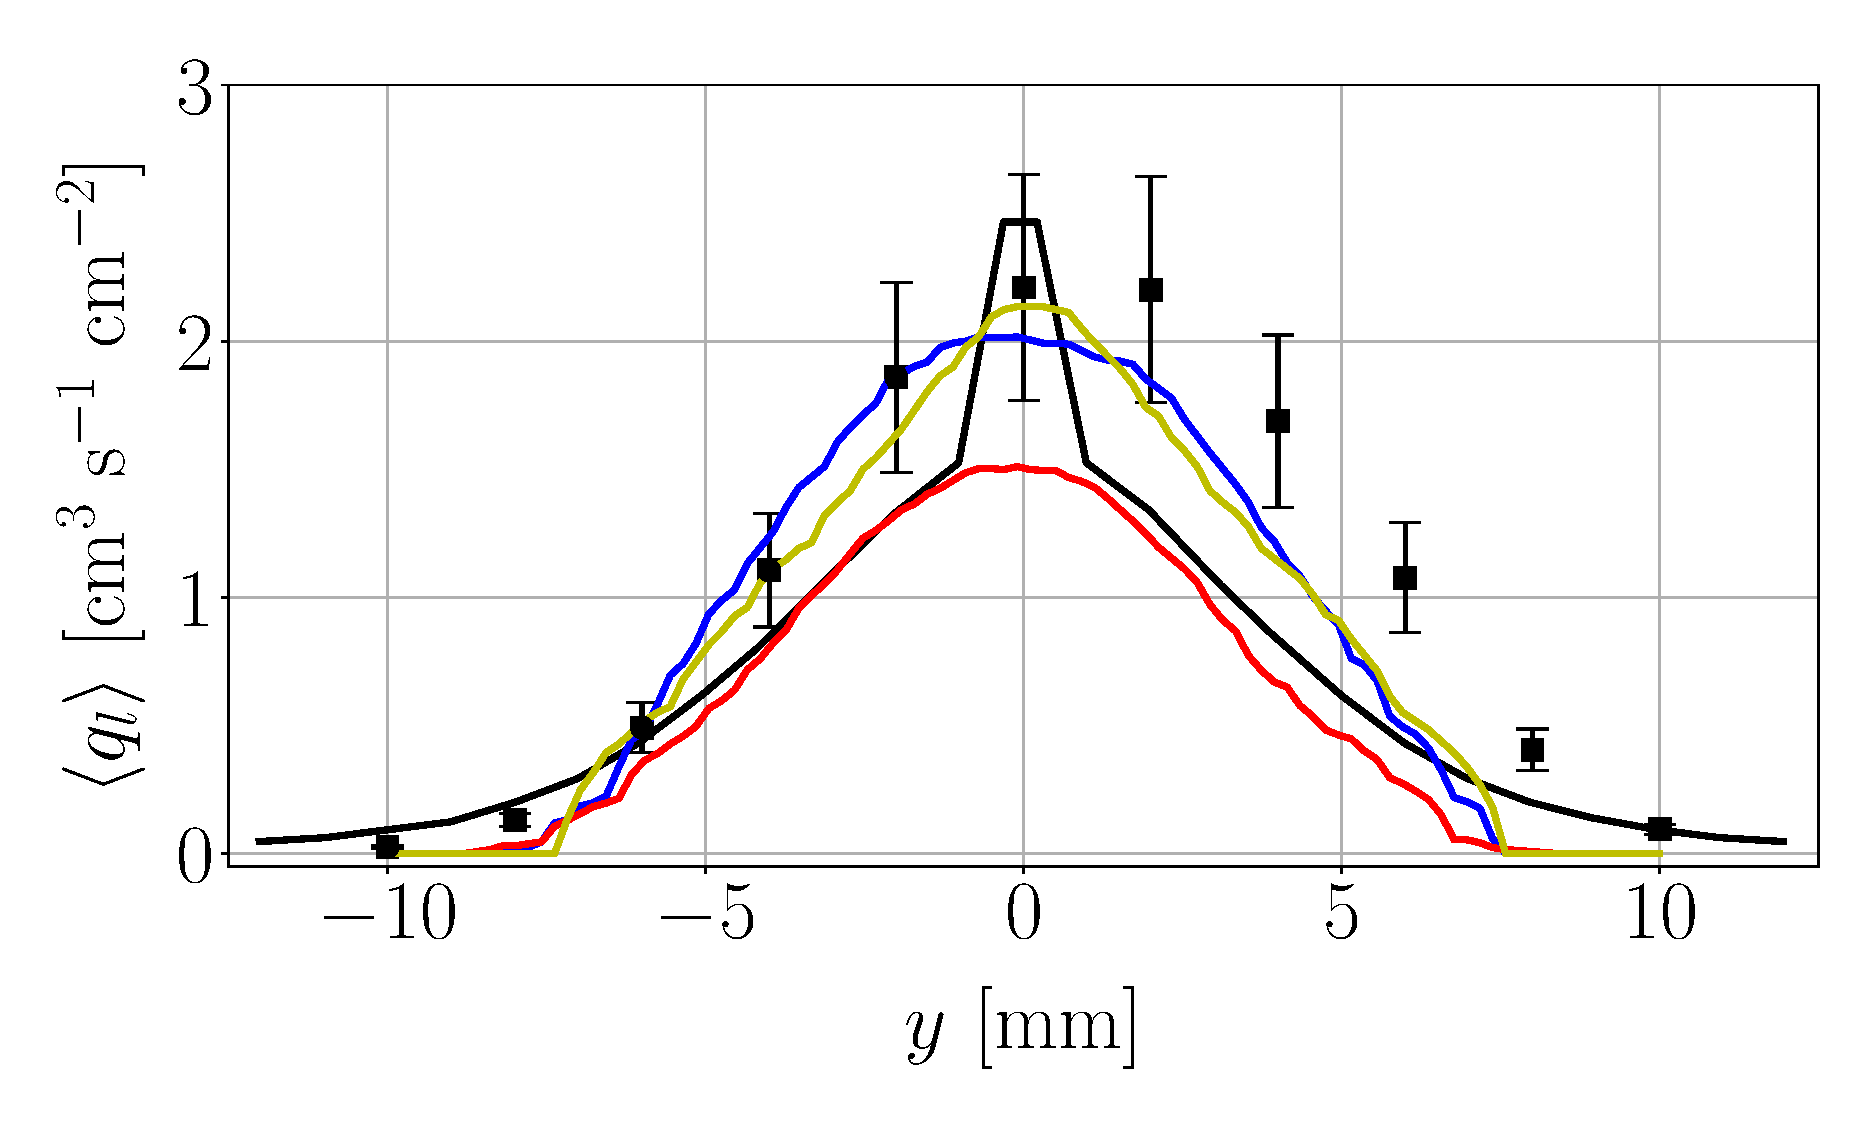
\includegraphics[scale=0.22]{./part2_developments/figures_ch6_lagrangian_JICF/previous_numerical_results/flux_profiles_along_y}
    %\hfill
   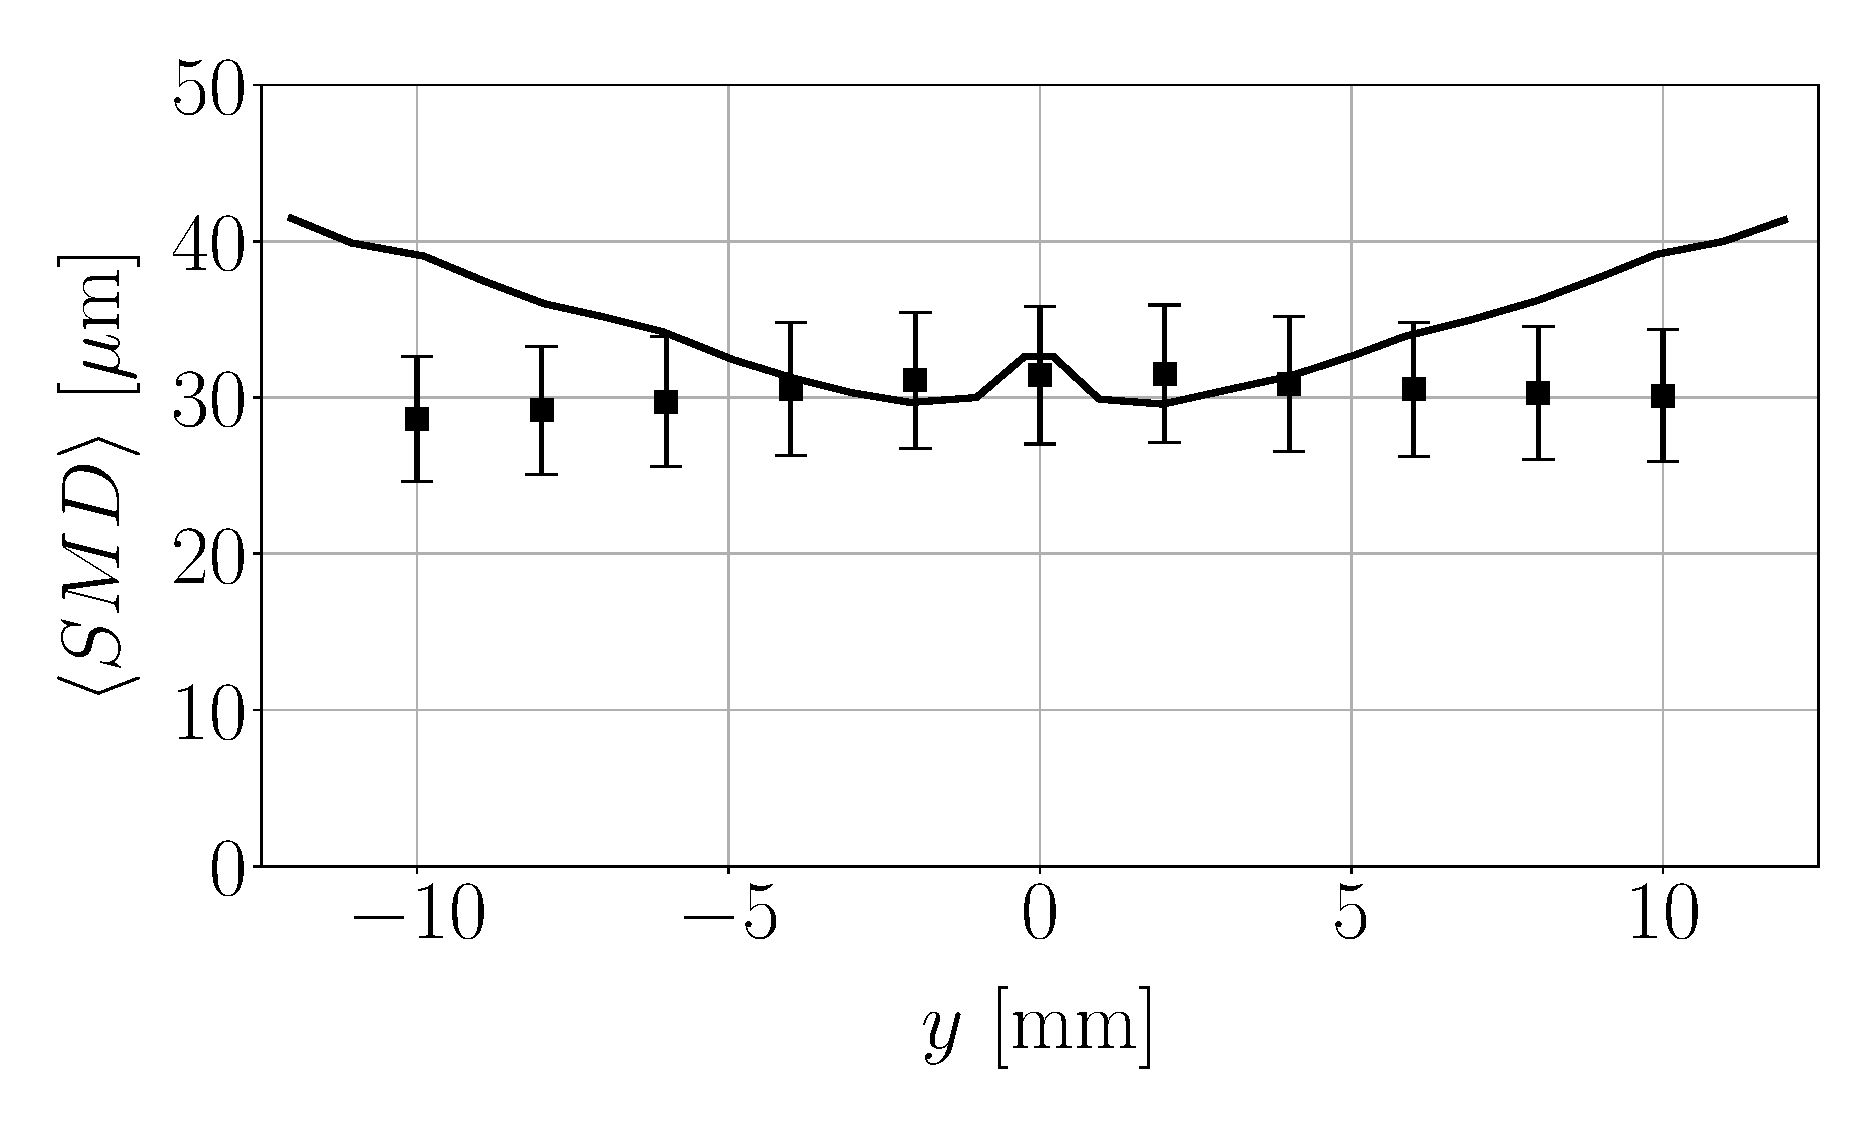
\includegraphics[scale=0.22]{./part2_developments/figures_ch6_lagrangian_JICF/previous_numerical_results/SMD_profiles_along_y}
   \caption{Profiles integrated over z}
   %\label{} 
\end{subfigure}
\caption{Integrated $SMD$ and volume flux profiles from experiments and past computational works. Computational fluxes have been obtained through digitalization and are hence not fully reliable }
\label{fig:previous_works_profiles_comparison_with_expe}
\end{figure}

\clearpage


\begin{table}[!h]
\centering
\caption{Global data obtained at $x = 80$ mm from experiments, previous computational studies and the present work}
\begin{tabular}{ccc}
\thickhline
Reference & $SMD~\left[ \mu \mathrm{m}\right]$  & $Q_l~\left[ \mathrm{mm}^3 s^{-1} \right]$ \\
\thickhline
\citeColor[becker_breakup_2002] & 31.0 &   4062  \\  
\citeColor[rachner_modelling_2002] & 31.9  & 3710  \\
\citeColor[jaegle_large_2009] & 33.2 &  3693.8  \\
\citeColor[senoner_simulation_2010] & 29.6  & 3573  \\
\citeColor[eckel_semi-empirical_2016] & 32.7  & 3775.9  \\
Present work & 19.44 & 3710 \\
\thickhline
\end{tabular}
\label{tab:previous_numerical_studies_on_jicf_dlr_values}
\end{table}


%\begin{table}[!h]
%\centering
%\caption{Data obtained from previous work }
%\begin{tabular}{ccccc}
%\thickhline
%Work & $SMD~\left[ \mu \mathrm{m}\right]$ & $\varepsilon_{SMD}~\left[\% \right]$ & $Q_l~\left[ \mathrm{mm}^3 s^{-1} \right]$ & $\varepsilon_{Q_l}~\left[ \% \right]$ \\
%\thickhline
%\citeColor[becker_breakup_2002] & 31 & &  4062&  \\  
%\citeColor[rachner_modelling_2002] & 31.9 & & 3710 & \\
%\citeColor[jaegle_large_2009] & 33.2 & & 3693.8 & \\
%\citeColor[senoner_simulation_2010] & 29.6 & & 3573 & \\
%\citeColor[eckel_semi-empirical_2016] & 32. & & 3775.9 & \\
%\thickhline
%\end{tabular}
%\label{tab:previous_numerical_studies_on_jicf_dlr_values}
%\end{table}

\vspace*{-0.2in}

\section{Procedure for parametric study of lagrangian simulations}


With the objective of testing all the parameters involved in the lagrangian computations, a design of experiments process is followed in which each variable is changed in a one-at-a-time basis. The study of dispersed-phase simulations in then divided into three parts, which are enclosed by the dashed-colored lines in Figure  \ref{fig:dispersed_phase_sli_parameters}:

\begin{enumerate}

	\item The \textbf{gaseous phase} effect is analyzed in $\S$\ref{sec:SLI_LGS_gaseous_phase_effect}. Firstly, two methodologies to model the perturbation effects created by the dense core are presented analyzed in gaseous simulations: the Actuator Line Method (ALM), whose modelling was detailed in $\S$\ref{sec:ch4_dense_core_modelling}, and another approach named prescribed gaseous inlet. Both methodologies are then tested in dispersed-phase simulations, where liquid is injected with the SLIs obtained from the resolved simulation UG100\_DX10 at $x = 5$ mm.
	
	\item The different \textbf{secondary atomization models} are analyzed in $\S$\ref{sec:SLI_LGS_secondary_breakup_models}. 
	
	\item The effects of the \textbf{liquid phase} parameters from SLI and operating conditions are reported in $\S$\ref{sec:effect_of_SLI_variables}. 

\end{enumerate}


\begin{figure}[ht]	
	\centering	\includeinkscape[inkscapelatex=false,scale=0.35]{./part2_developments/figures_ch6_lagrangian_JICF/chart_input_parameters_LGS}
	\caption{Schematic of parameters involved in SLI simulations and their interactions}	\label{fig:dispersed_phase_sli_parameters}
\end{figure}



\section{Influence of gaseous phase}
\label{sec:SLI_LGS_gaseous_phase_effect}


\subsection{Computational setups and boundary conditions}
\label{sec:ch6_BC_gaseous_phase}

In this section, the influence of the gaseous phase in the dispersed-phase simulation is analyzed. Two computational setups with two different modeling methodologies for replicating the perturbed gaseous phase are detailed. The first one employs \textbf{Actuator Line Method} (ALM), detailed in $\S$\ref{sec:ch4_dense_core_modelling}, while the second one consists of \textbf{prescribing gaseous phase} statistics on a reduced domain representing the plenum downstream the liquid injection nozzle location. The gaseous fields generated by both methodologies are firstly analyzed, followed by dispersed-phase computations performed with both methodologies.

\clearpage


\subsubsection*{Actuator Line Method}



To mimic the perturbation phase created by the crossflow with ALM, the same computational geometry as the one used by the resolved simulations from Chapter \ref{ch5:jicf_resolved_simulations} is used (Figure \ref{fig:numerical_setup_maquette_JICF_DLR}).    In the mesh from these resolved computations, an element size of $\Delta x = 0.5$ mm was prescribed upstream the liquid nozzle, since it could transport the prescribed turbulence ($\S$\ref{sec:ch5_initial_conditions}). In dispersed-phase simulations, the region of interest extends up to a location at $x = 80$ mm downstream the injector, which corresponds to the location where the experiments from \citeColor[becker_breakup_2002] report results on fluxes and SMD. Therefore, these simulations use a baseline cell size of $\Delta x = 0.5$ mm in the plenum from the gaseous inlet up to $x = 85$ mm downstream the injector in order to allow for turbulent transport up to the experimental validation plane (located at $x = 80$ mm). The mesh, shown in Figure \ref{fig:jicf_dlr_mesh_LGS}, consists of $74 \cdot 10^6$ elements, hence being firstly heavier than the baseline mesh employed for the resolved simulations but eventually lighter due to the lack of AMR. Droplets are injected in this mesh as lagrangian point-particles whose dynamics follow the equations from  $\S$\ref{sec:ch3_EL_formalisms}. %The energy equation is not considered since the test bench is at ambient temperature and evaporation does not take place.


\begin{figure}[h!]
	\centering	\includeinkscape[inkscapelatex=false,scale=0.8]{./part2_developments/figures_ch6_lagrangian_JICF/jicf_mesh_LGS}
	\vspace*{-0.1in}
	\caption{Mesh employed for dispersed-phase simulations with ALM}
	\label{fig:jicf_dlr_mesh_LGS}
\end{figure}

%\subsection{Setup of actuator model}

For gaseous phase perturbation, an actuator can be defined in the numerical domain with the control parameters from Table \ref{tab:alm_parameters}. An example of an actuator representing the dense core in a gaseous simulations can be seen in Figure \ref{fig:u_inst_SPS_and_ALM}. This one is graphically represented as a cylinder extending from the injection nozzle exit (initial point) up to the dense core breakup point (end point), which is estimated from the resolved simulations. The actuator points (not shown in the figure) are disseminated uniformly along the central line of the cylinder. The discrete forces applied to each point are then mollified in the neighbouring cells in order to avoid flow singularities. 

To assess the ALM, the results from the high Weber operating point (Table \ref{tab:jicf_operating_conditions}) for the fine case (UG100\_DX10) are used. The actuator point coordinates $x_b$, $z_b$ are obtained from the mean values of Figure \ref{fig:dense_core_mean_parameters_scatterplots}, while the force $F_\mathrm{DC}$ is taken from Table \ref{tab:dense_core_geometry_pressures_and_force_parameters}. These values, summarized in Table \ref{tab:jicf_lgs_ALM_parameters}, represent an \textbf{initial} actuator. As it will be shown, it was found that the disturbance effect created by this actuator was not optimal to replicate the perturbations from the resolved simulation. Thus, the ALM control variables were tuned until finding an actuator which was found to better match the perturbed gaseous field: this one is summarized as the \textbf{optimal} actuator from Table \ref{tab:jicf_lgs_ALM_parameters}. Besides from this optimal actuator, two other configurations are also reported to illustrate the influence of the parameters: one which takes the end point of the optimal actuator and the net force of the initial one (\textbf{ALM tilted}), and another one which takes the optimal end point but increases the net force (\textbf{ALM forced}). 




\begin{figure}[h!]
	\centering	\includeinkscape[inkscapelatex=false,scale=0.6]{./part2_developments/figures_ch6_lagrangian_JICF/gas_field_initial_conditions/u_inst_SPS_and_ALM}
	\caption[Perturbation effect towards the gaseous phase visualized through the instantaneous velocity magnitude in the plane $y = 0$]{Perturbation effect towards the gaseous phase visualized through the instantaneous velocity magnitude in the plane $y = 0$. The snapshots correspond to the resolved simulation UG100\_DX10 (\textsl{left}) and to a gaseous simulation with the optimal actuator (\textsl{right})}	
	\label{fig:u_inst_SPS_and_ALM}
\end{figure}


\clearpage

\begin{table}[!h]
\centering
\caption{Parameters of an actuator representing the dense core for the high Weber case}
\begin{tabular}{cccccc}
\thickhline
\textbf{Parameter} & \textbf{Units} &  \textbf{ALM Initial} & \textbf{ALM tilted} &  \textbf{ALM optimal} & \textbf{ALM forced} \\
\thickhline
$x_b$ & mm & 2.46 & 1.5 & 1.5 & 1.5 \\
$z_b$ & mm & 3.07 & 3.0 & 3.0 & 3.0 \\
%$c_0$ & mm & 0.45 & 0.45 \\
%$c_L$ & mm & & \\
$| \textbf{F}_\mathrm{DC} |$ & N & 0.095 & 0.095 & 0.25 & 0.30 \\
%$\Delta p$ & Pa &  & \\
\thickhline
\end{tabular}
\label{tab:jicf_lgs_ALM_parameters}
\end{table}




% Initial: L = 3.934 mm, L/2 = 1.967 mm, theta = 38.71
% Final: L = 3.354 mm, L/2 = 1.677 mm, theta = 26.565



In first place, the mean axial velocity fields in the symmetry plane $y = 0$ are shown in Figure \ref{fig:ALM_gas_fields_plane_Y}. The resolved case UG100\_DX10 is also displayed for comparison.  As observed, the initial actuator model creates only a slight perturbation downstream the cylinder location, but cannot properly retrieve the recirculation and deceleration captured by the resolved simulation. By changing only the actuator coordinates (tilted configuration), the perturbation effect is intensified and more distributed in space: since the angle $\theta$ increases, the imposed drag reduces augments while the lift reduces (Eqs. (\ref{eq:ALM_SLI_lift_drag_definitions})). This effect is also reflected in the mean velocity profiles of Figures \ref{fig:JICF_ICS_ALM_lines_y0_along_x_ux_mean} and \ref{fig:JICF_ICS_ALM_lines_y0_along_z_ux_mean}: the tilted profile reduces the gaseous velocity more than the initial one, even though its perturbation is not yet close to the resolved profile. Indeed, the lift force imposed is not large enough and streamlines do not deviate towards the vertical direction as in the resolved case, staying oriented towards the crossflow direction as in the unperturbed case. If the net force is now increased (optimal configuration),  Figure \ref{fig:ALM_gas_fields_plane_Y} shows that the axial velocity decreases downstream the ALM region, with an increase also in the lift force as in this case streamlines are deviated upwards. The velocity profiles from Figures \ref{fig:JICF_ICS_ALM_lines_y0_along_x_ux_mean} and \ref{fig:JICF_ICS_ALM_lines_y0_along_z_ux_mean} show this greater perturbation when compared to the previous cases. Nevertheless, the disturbance is still not strong enough to capture the recirculation bubble from the resolved simulation. A further increase in the net force imposed (forced configuration) shows effectively a larger perturbation which can actually capture a recirculation bubble behind the ALM region, even though its location is shifted upwards with respect to resolved simulation. The  velocity profiles from Figures \ref{fig:JICF_ICS_ALM_lines_y0_along_x_ux_mean} and \ref{fig:JICF_ICS_ALM_lines_y0_along_z_ux_mean} also reflect this larger perturbation. However, even if the forced configuration case seems to retrieve better the gaseous field a priori, its stronger perturbation was found to greatly affect secondary atomization of the droplets in dispersed-phase simulations, yielding very small droplets. The configuration reported as optimal yielded the best spray results among all the ALM cases tested. %Forces in between the ones corresponding to the optimal and forced configurations were also tested (not reported here), without improving the dispersed-phase results.







\begin{figure}[h!]	
	\centering	\includeinkscape[inkscapelatex=false,scale=0.225]{./part2_developments/figures_ch6_lagrangian_JICF/gas_field_initial_conditions/ALM_planes_y}
	\vspace*{-0.1in}
	\caption{Mean axial velocity field at plane $y = 0$ for resolved case UG100\_DX10 and the three actuators tested. The grey cylinder represents the actuator, i.e. the location where body forces are applied}
	\label{fig:ALM_gas_fields_plane_Y}
\end{figure}

\clearpage

\begin{figure}[ht]
\flushleft
\begin{subfigure}[b]{0.45\textwidth}
	\centering
   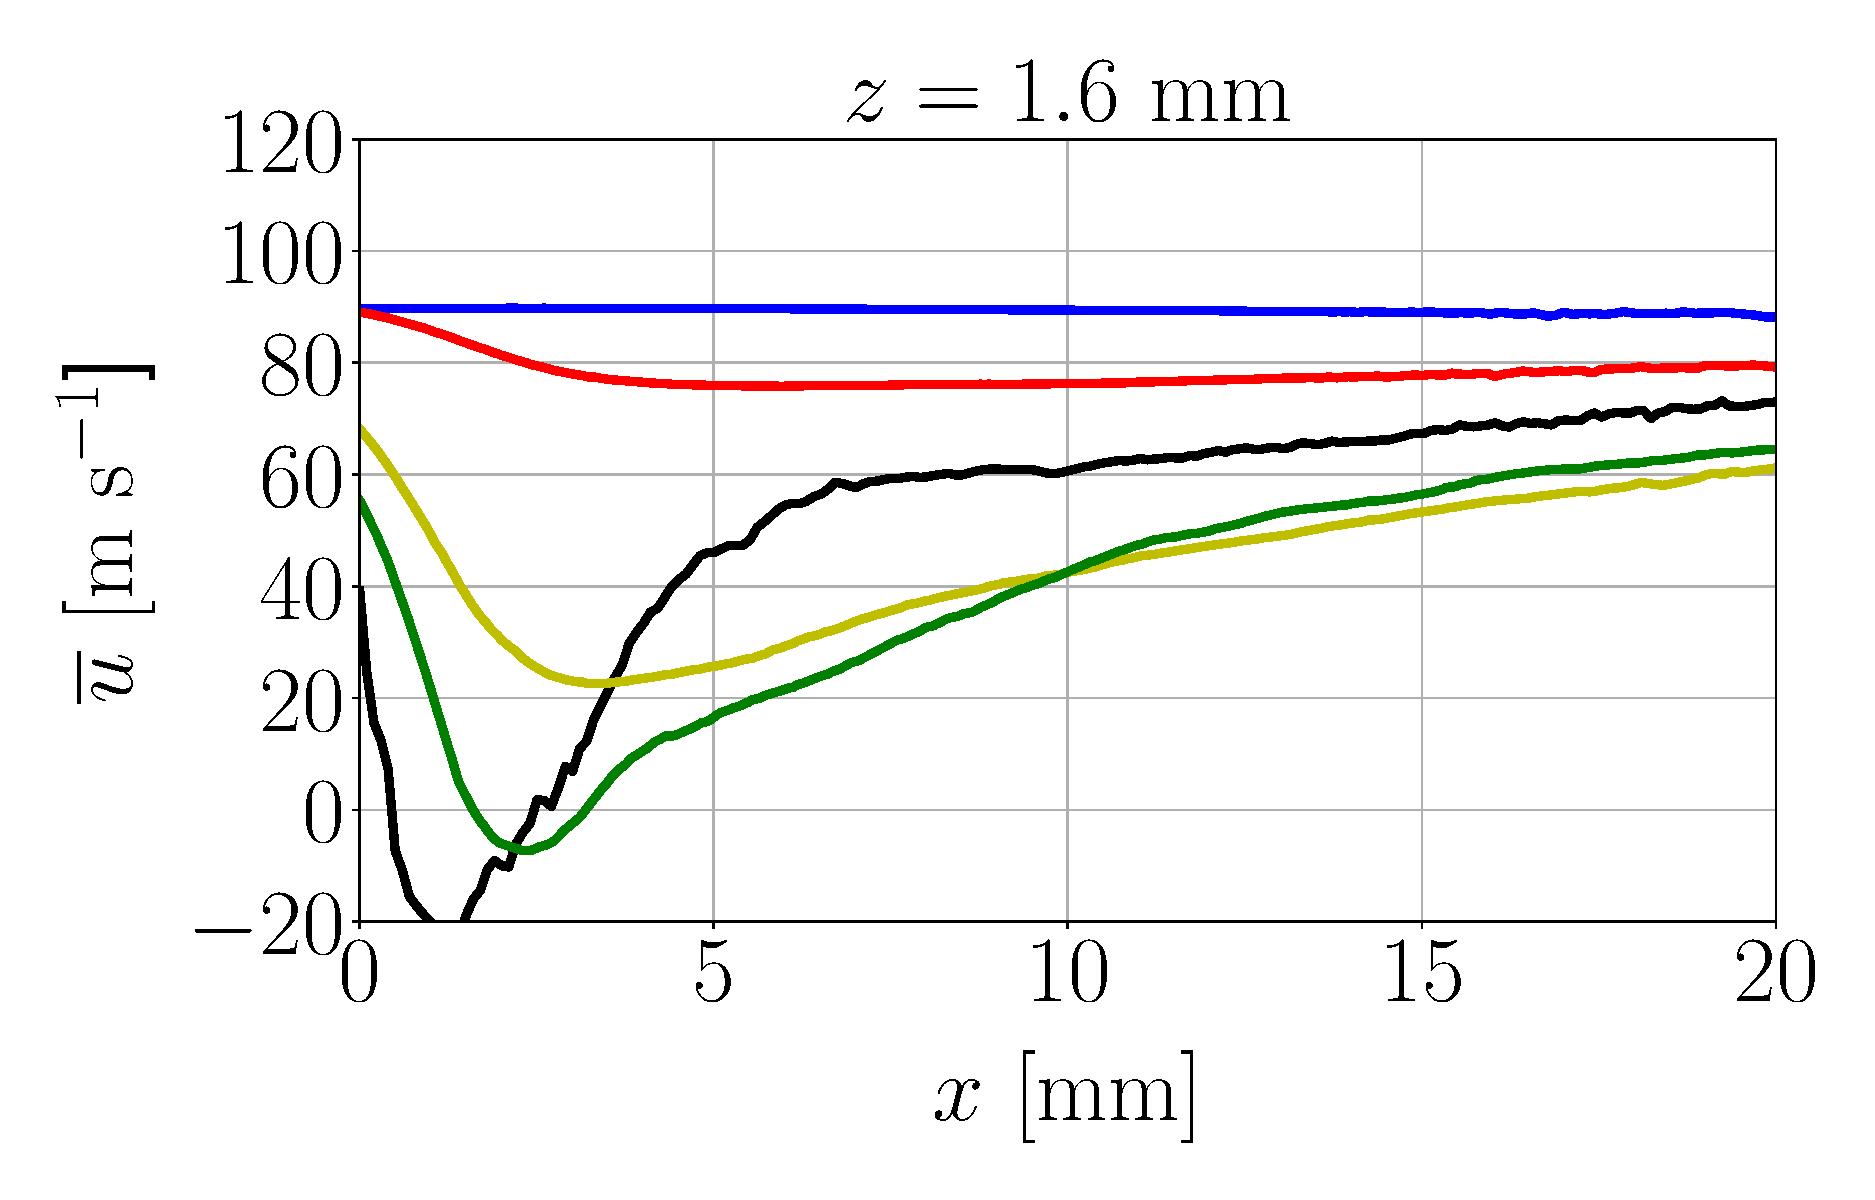
\includegraphics[scale=0.25]{./part2_developments/figures_ch6_lagrangian_JICF/gas_field_initial_conditions/ALM_line_y0_along_x_z01p6}
   %\caption{}
   %\label{} 
\end{subfigure}
\hspace{0.4in}
\begin{subfigure}[b]{0.45\textwidth}
	\centering
   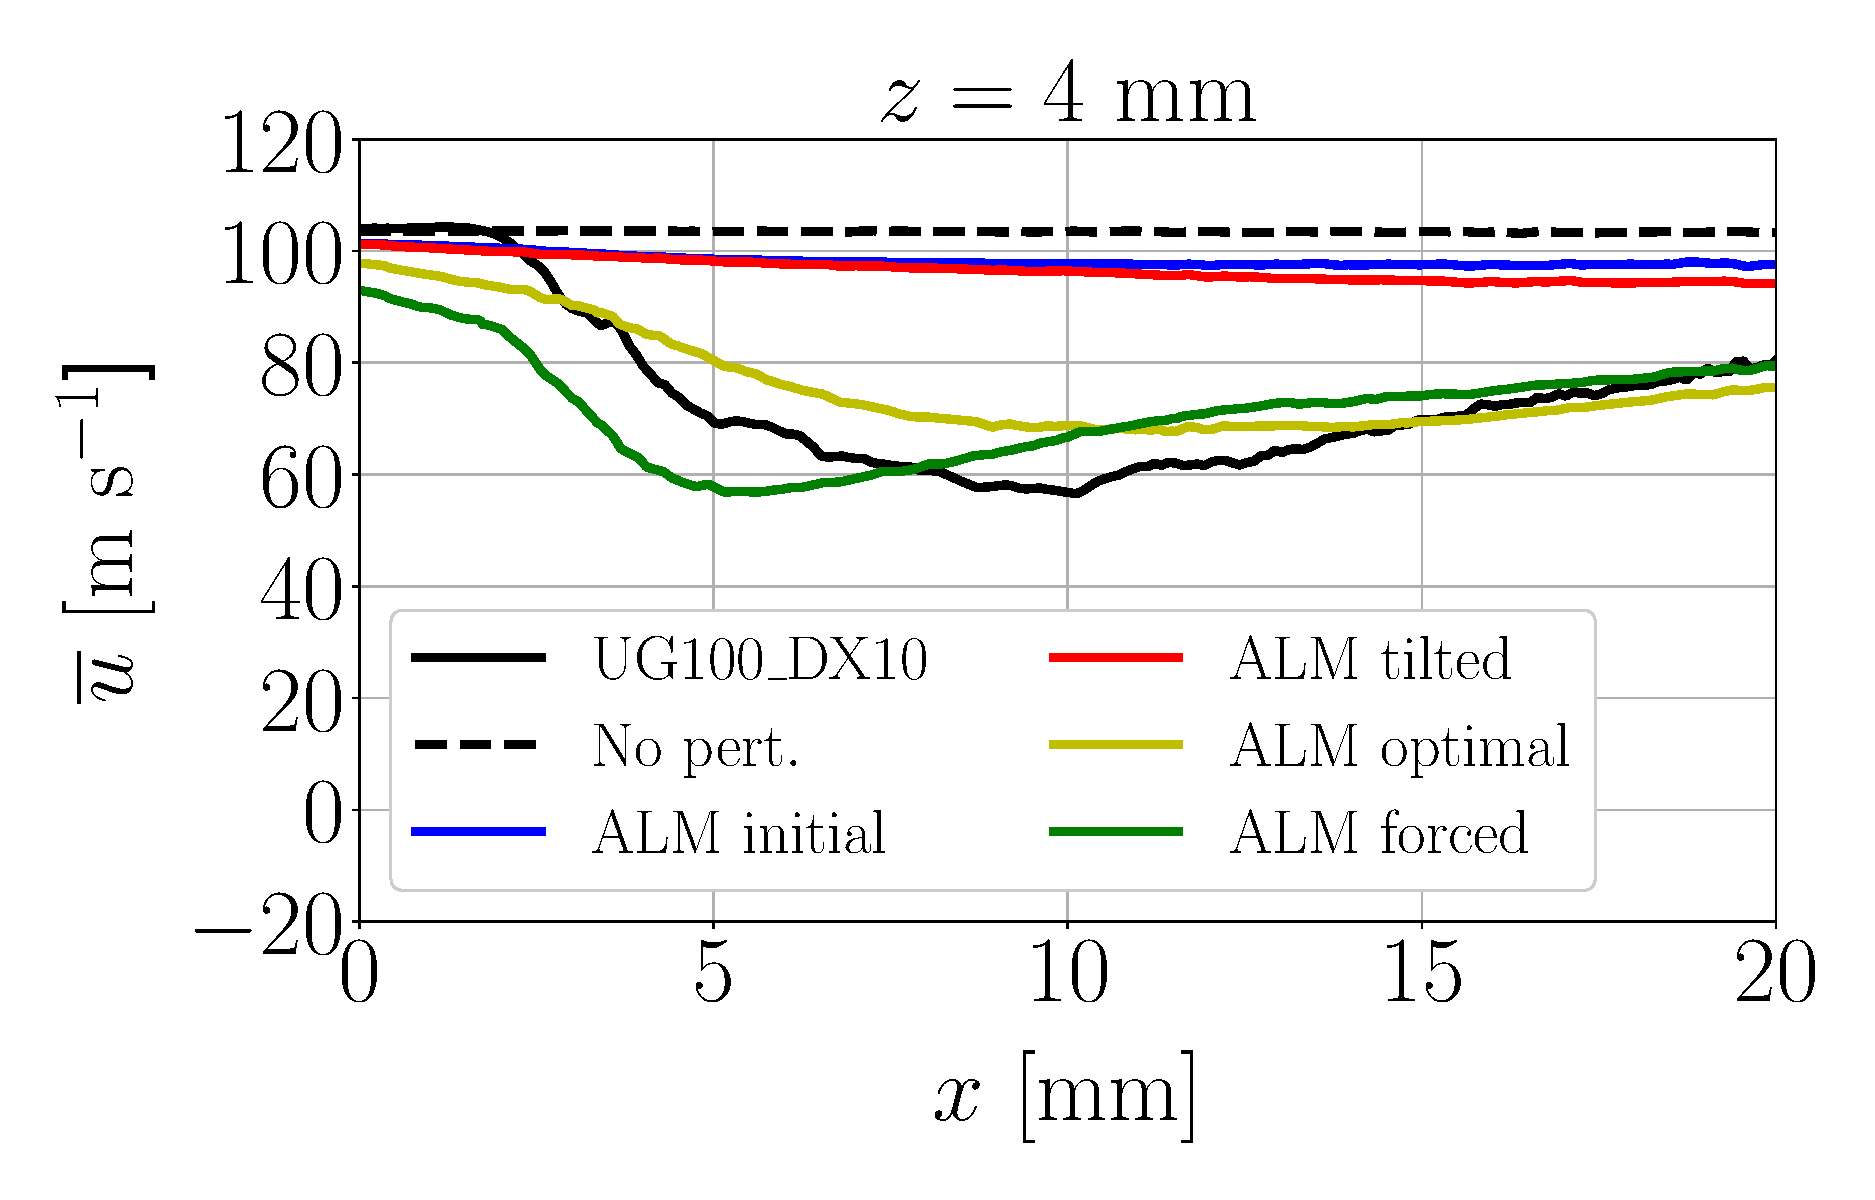
\includegraphics[scale=0.25]{./part2_developments/figures_ch6_lagrangian_JICF/gas_field_initial_conditions/ALM_line_y0_along_x_z04p0}
   %\caption{}
   %\label{}
\end{subfigure}
\vspace*{-0.15in}
\caption{Mean axial velocity evolution in ALM and resolved simulations along axial coordinate at locations $z = 1.6, 4$ mm in plane $y = 0$ (lines of Figure \ref{fig:ALM_gas_fields_plane_Y})}
\label{fig:JICF_ICS_ALM_lines_y0_along_x_ux_mean}
\end{figure}




\begin{figure}[ht]
\centering
   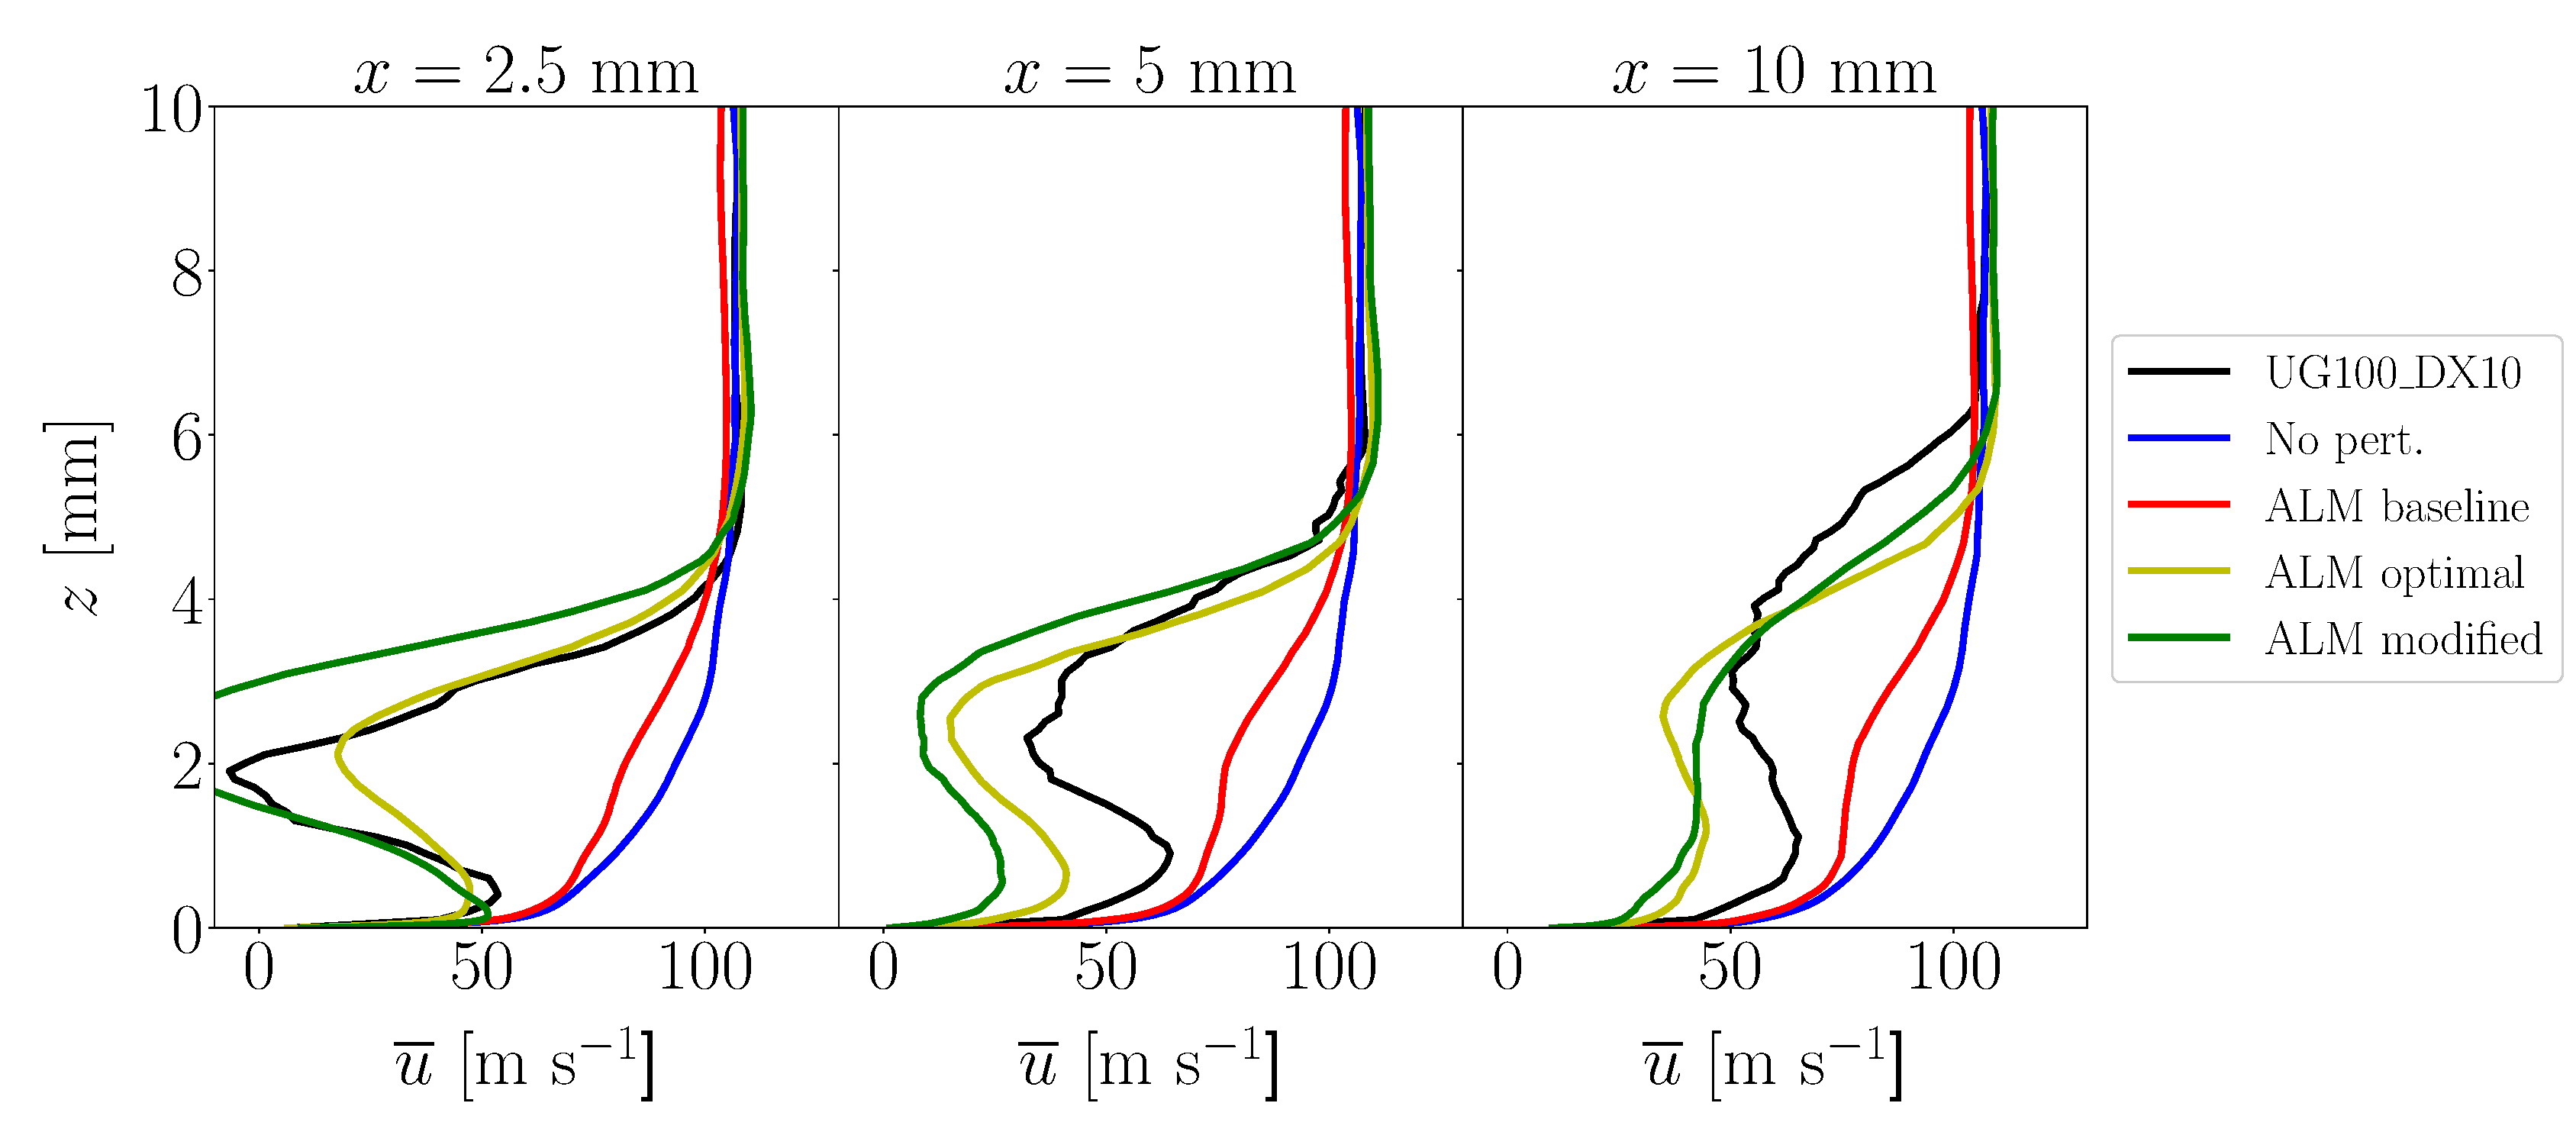
\includegraphics[scale=0.26]{./part2_developments/figures_ch6_lagrangian_JICF/gas_field_initial_conditions/ALM_lines_y0_along_z_ux_mean}
   \vspace*{-0.2in}
\caption{Mean axial velocity evolution in ALM and resolved simulations along vertical coordinate at $x = 2.5, 5, 10$ mm locations of plane $y = 0$ (lines of Figure \ref{fig:ALM_gas_fields_plane_Y})}
\label{fig:JICF_ICS_ALM_lines_y0_along_z_ux_mean}
\end{figure}


Since the purpose of ALM is to mimic the gaseous perturbations generated by the dense core, it is also of interest to look at the planes perpendicular to the crossflow. Figure \ref{fig:ALM_gas_fields_plane_x} shows the mean velocity fields at planes $x = 5, 10$ mm compared to the resolved cases. Modifying the actuator ending coordinates and increasing the net dense core reduces further the mean velocities in the flow field. This has also a strong effect in the Counter-Rotating Vortices (CRVs), which can affect the transport and atomization of the droplets. Cases unperturbed and initial ALM do not show CRVs in the flow as shown by the streamlines, while the tilted and optimal ALM cases can retrieve quite accurately the location, intensity and rotation direction of the resolved vortices. Further increasing the net force shows still vortical structures, yet these are small and differ from the shape of the resolved ones. %In fact, a further increase in the force (not reported here) was also checked and showed that the CRVs inverted their rotation direction, which is an unphysical behaviour in the JICF \citepColor[karagozian_analytical_1986].

\clearpage

\begin{figure}[h!]	
	\centering	\includeinkscape[inkscapelatex=false,scale=0.205]{./part2_developments/figures_ch6_lagrangian_JICF/gas_field_initial_conditions/ALM_planes_x}
	\caption{Mean axial velocity field at planes $x = 5, 10$ mm for resolved case UG100\_DX10 and gaseous cases with and without ALM}
	\label{fig:ALM_gas_fields_plane_x}
\end{figure}

\clearpage

Finally, the velocity profiles along the white lines from Figure \ref{fig:ALM_gas_fields_plane_x} are plotted in Figure \ref{fig:JICF_ALM_lines_iso-x_along_y_ux_mean}. Again, the initial and tilted ALM do not create in general a noticeable disturbance in the flow field compared to the resolved case, except at $z = 1.6$ mm in plane $x = 10$ mm where the tilted case shows the closest match of all models. Increasing the force approaches the resolved perturbation at plane $x = 5$ mm: the optimal ALM shows a good match at $z = 1.6$ mm, while the equivalent occurs for the forced ALM further away from the wall at $z = 5$ mm. For the profiles at $z = 5$ mm in plane $x = 10$ mm, none of the actuators could achieve the intensity of the resolved perturbation: all actuators create the greatest perturbations downstream the actuator region but has a very limited influence further vertically from its ending point, which is not the case of a resolved dense core since the ligaments created during primary atomization also create perturbations in the gas field away from the dense core. 




\begin{figure}[ht]
\centering
\begin{subfigure}[b]{1.0\textwidth}
	\centering
   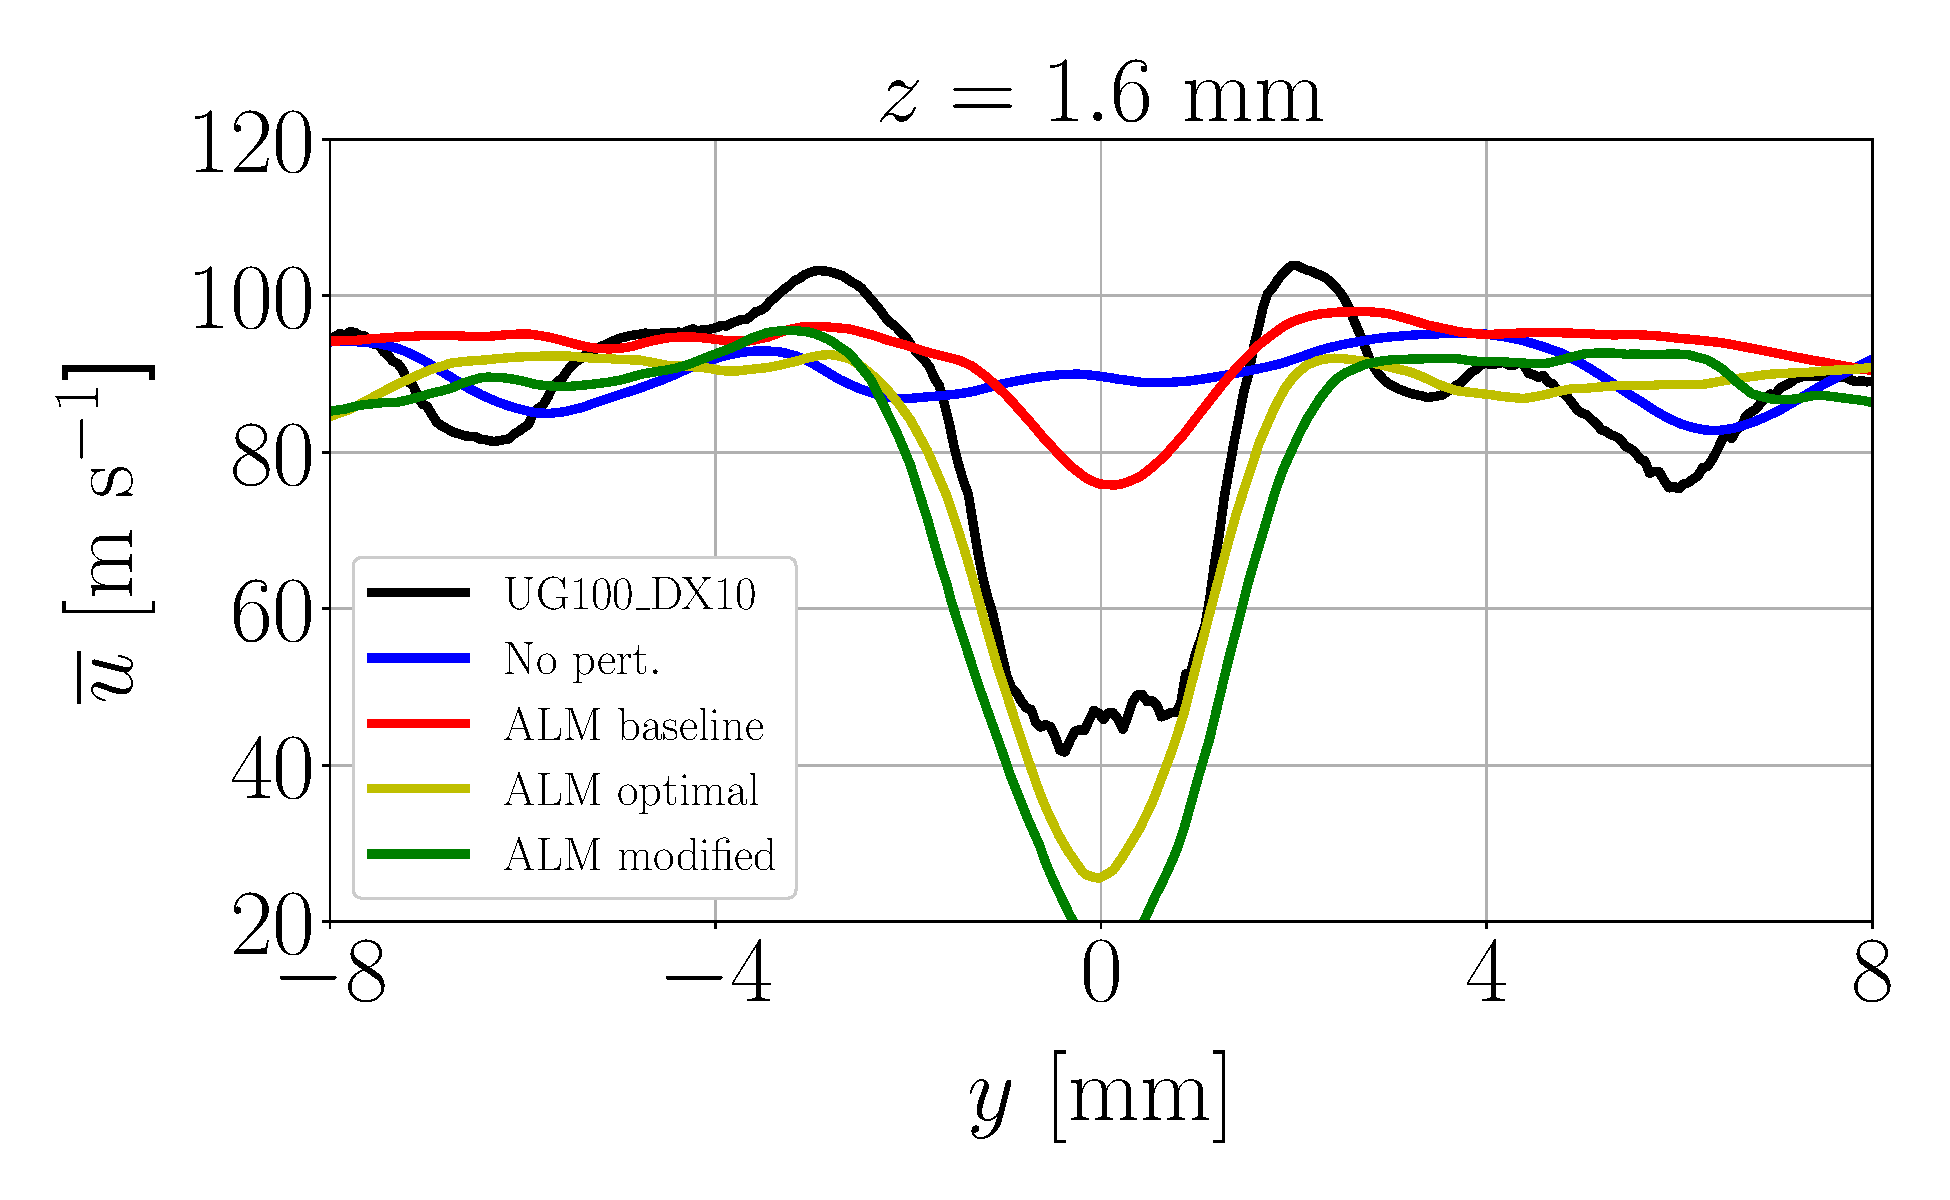
\includegraphics[scale=0.24]{./part2_developments/figures_ch6_lagrangian_JICF/gas_field_initial_conditions/ALM_line_x05_z01p6_ux_mean_along_y}
   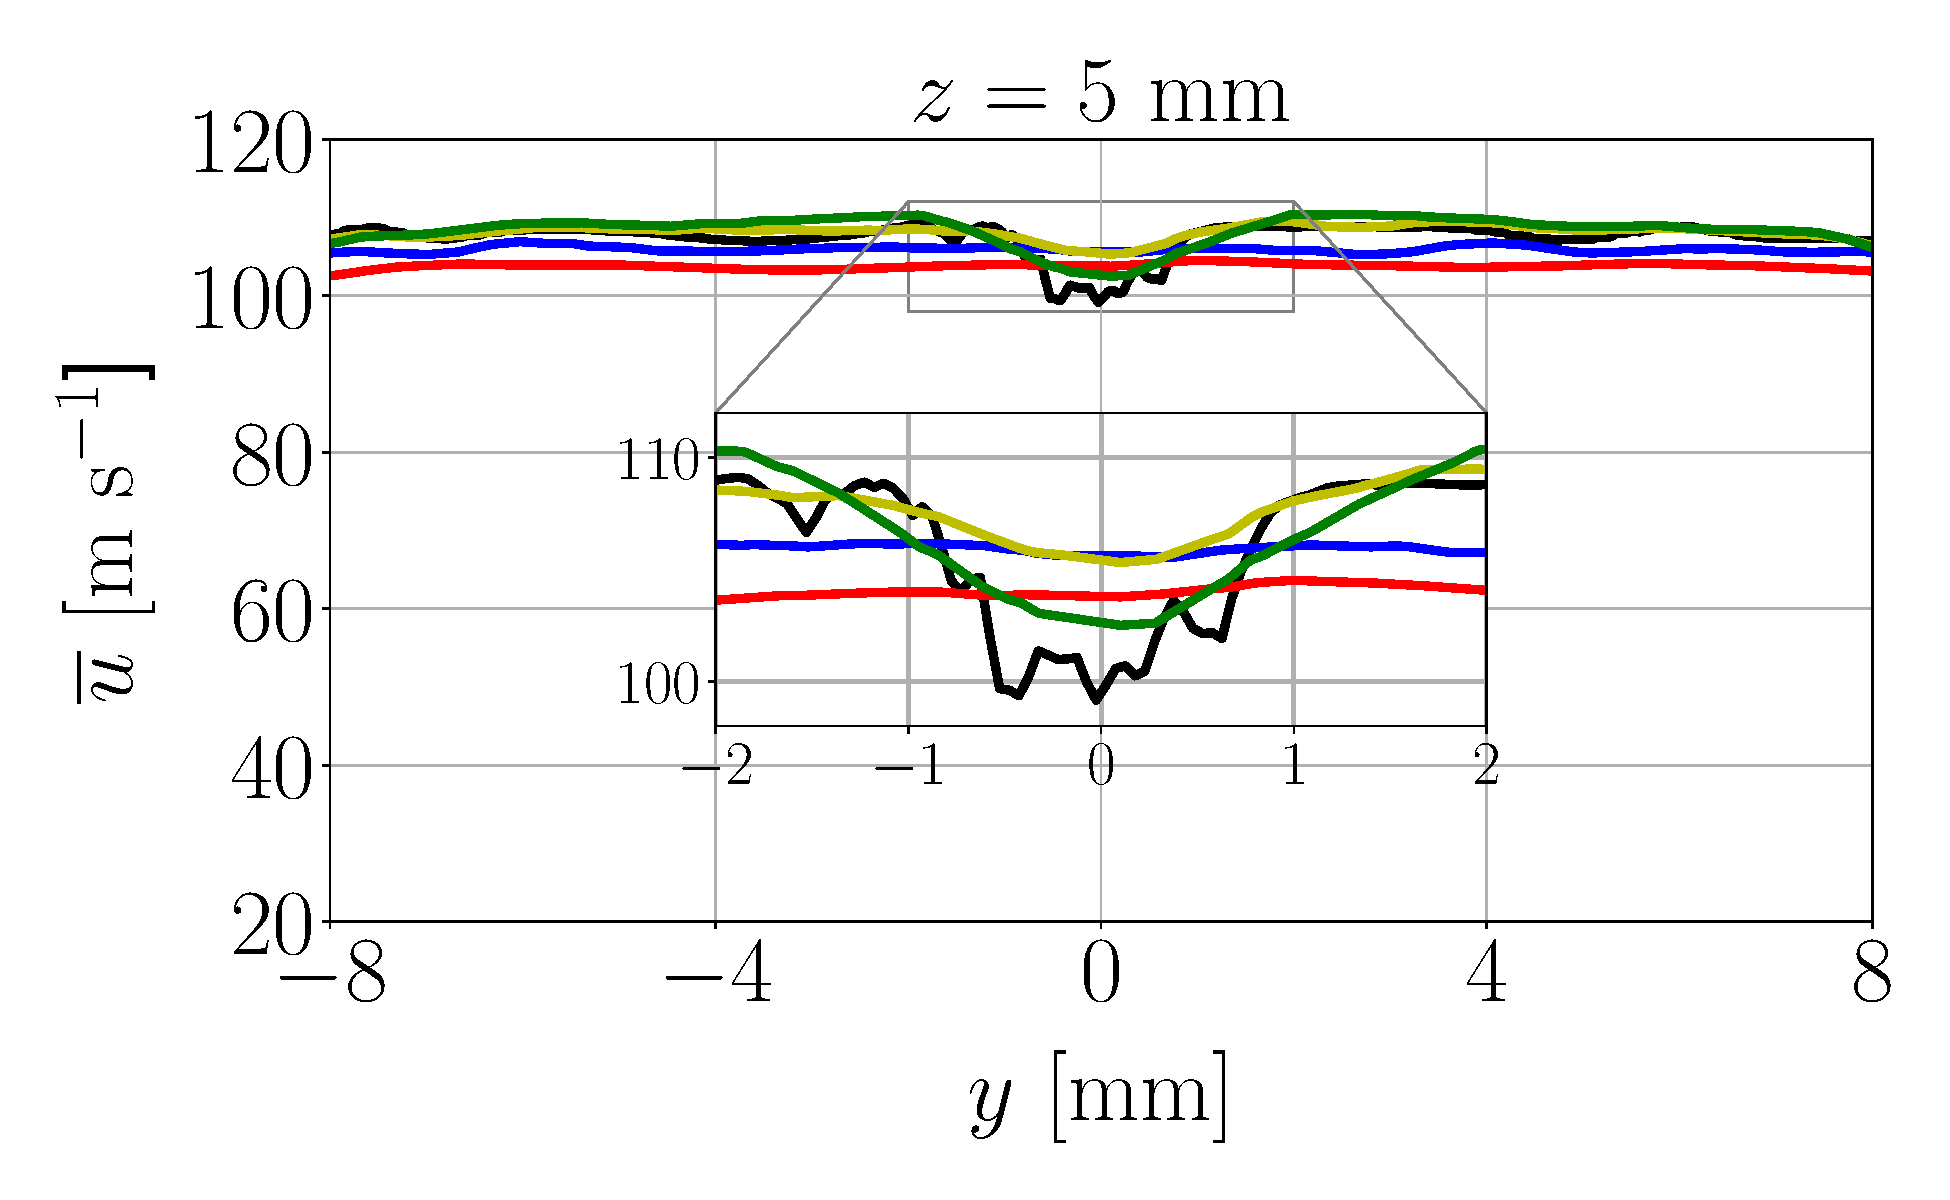
\includegraphics[scale=0.24]{./part2_developments/figures_ch6_lagrangian_JICF/gas_field_initial_conditions/ALM_line_x05_z05p0_ux_mean_along_y}
   \vspace*{-0.1in}
	\caption{Plane $x = 5$ mm}
\end{subfigure}
\vskip\baselineskip
\begin{subfigure}[b]{1.0\textwidth}
	\centering
   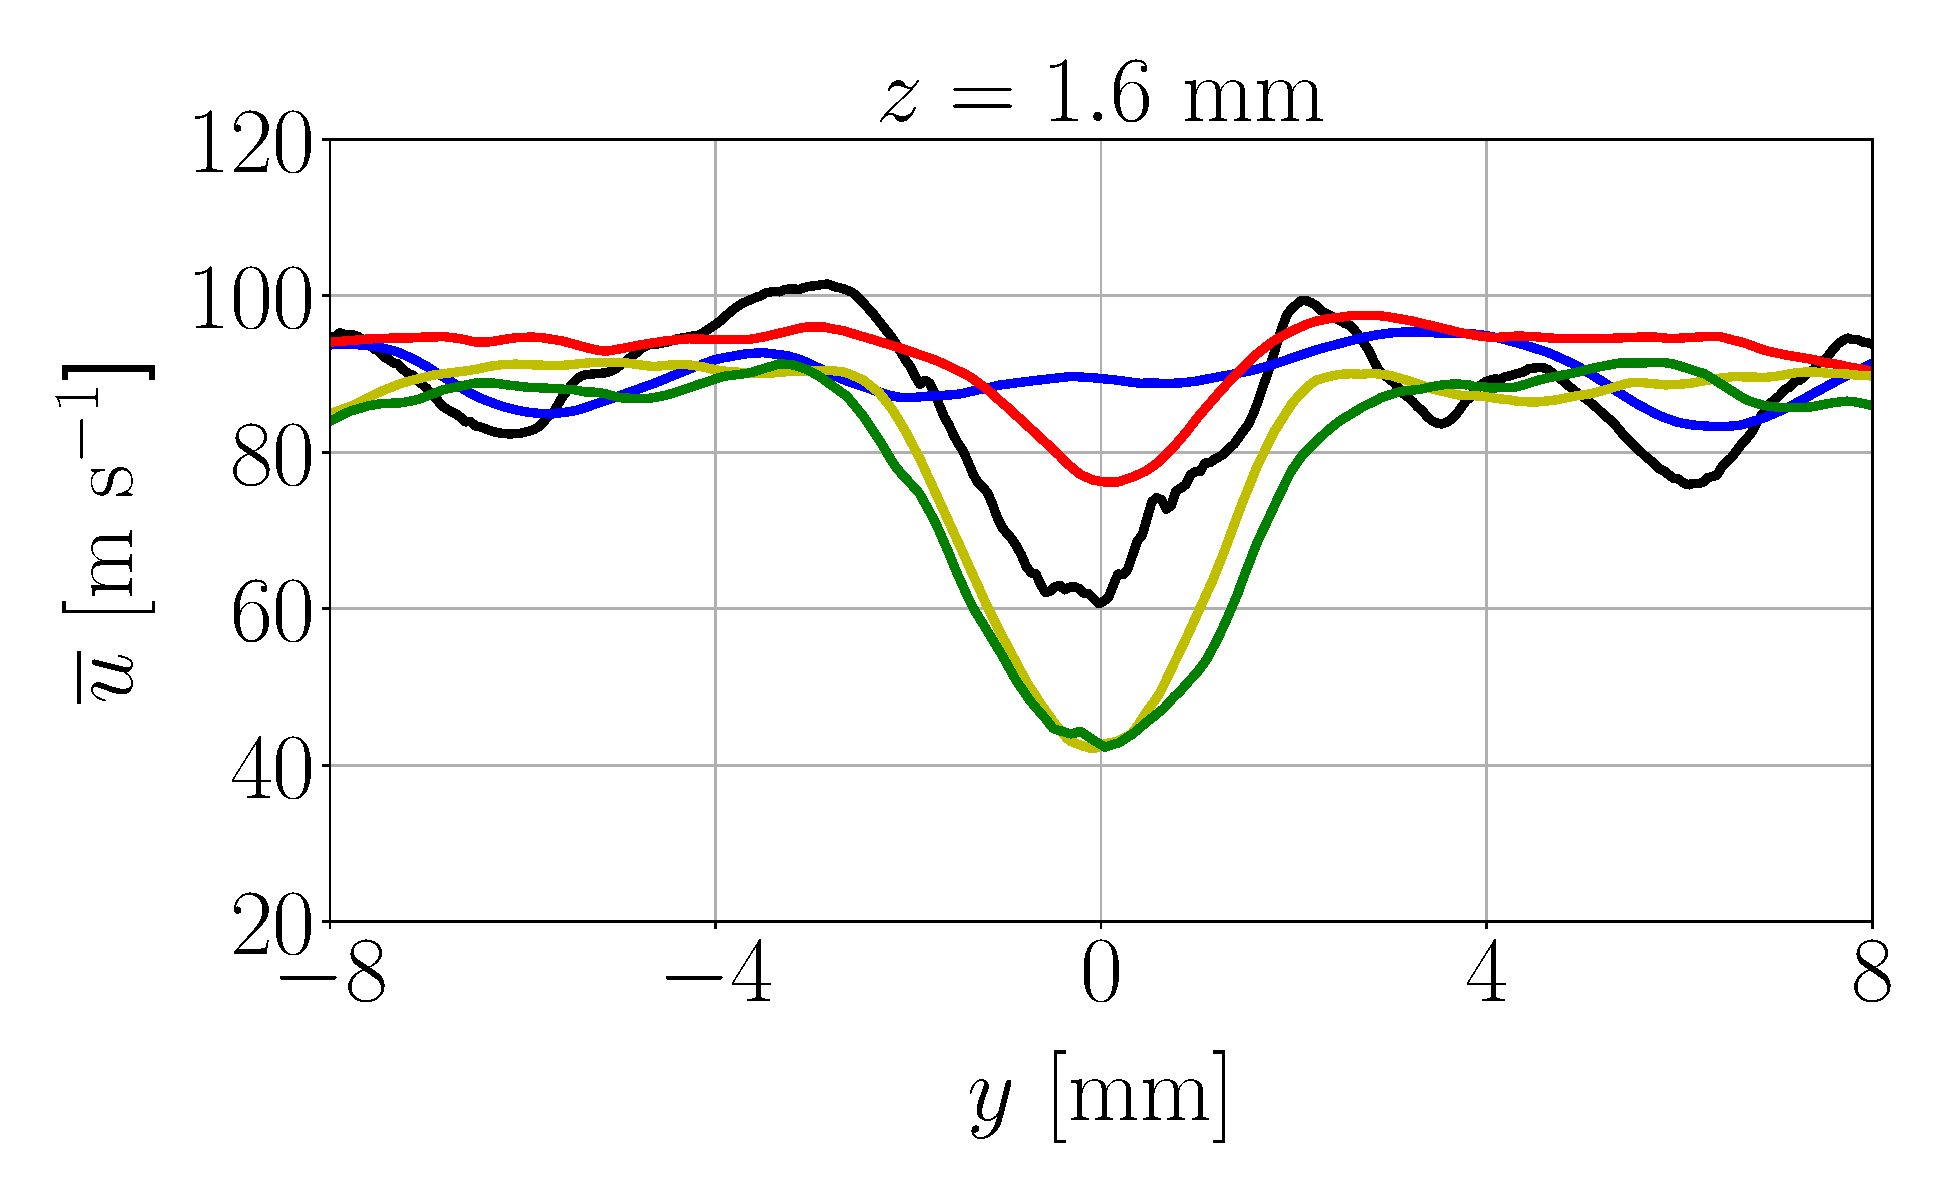
\includegraphics[scale=0.24]{./part2_developments/figures_ch6_lagrangian_JICF/gas_field_initial_conditions/ALM_line_x10_z01p6_ux_mean_along_y}
   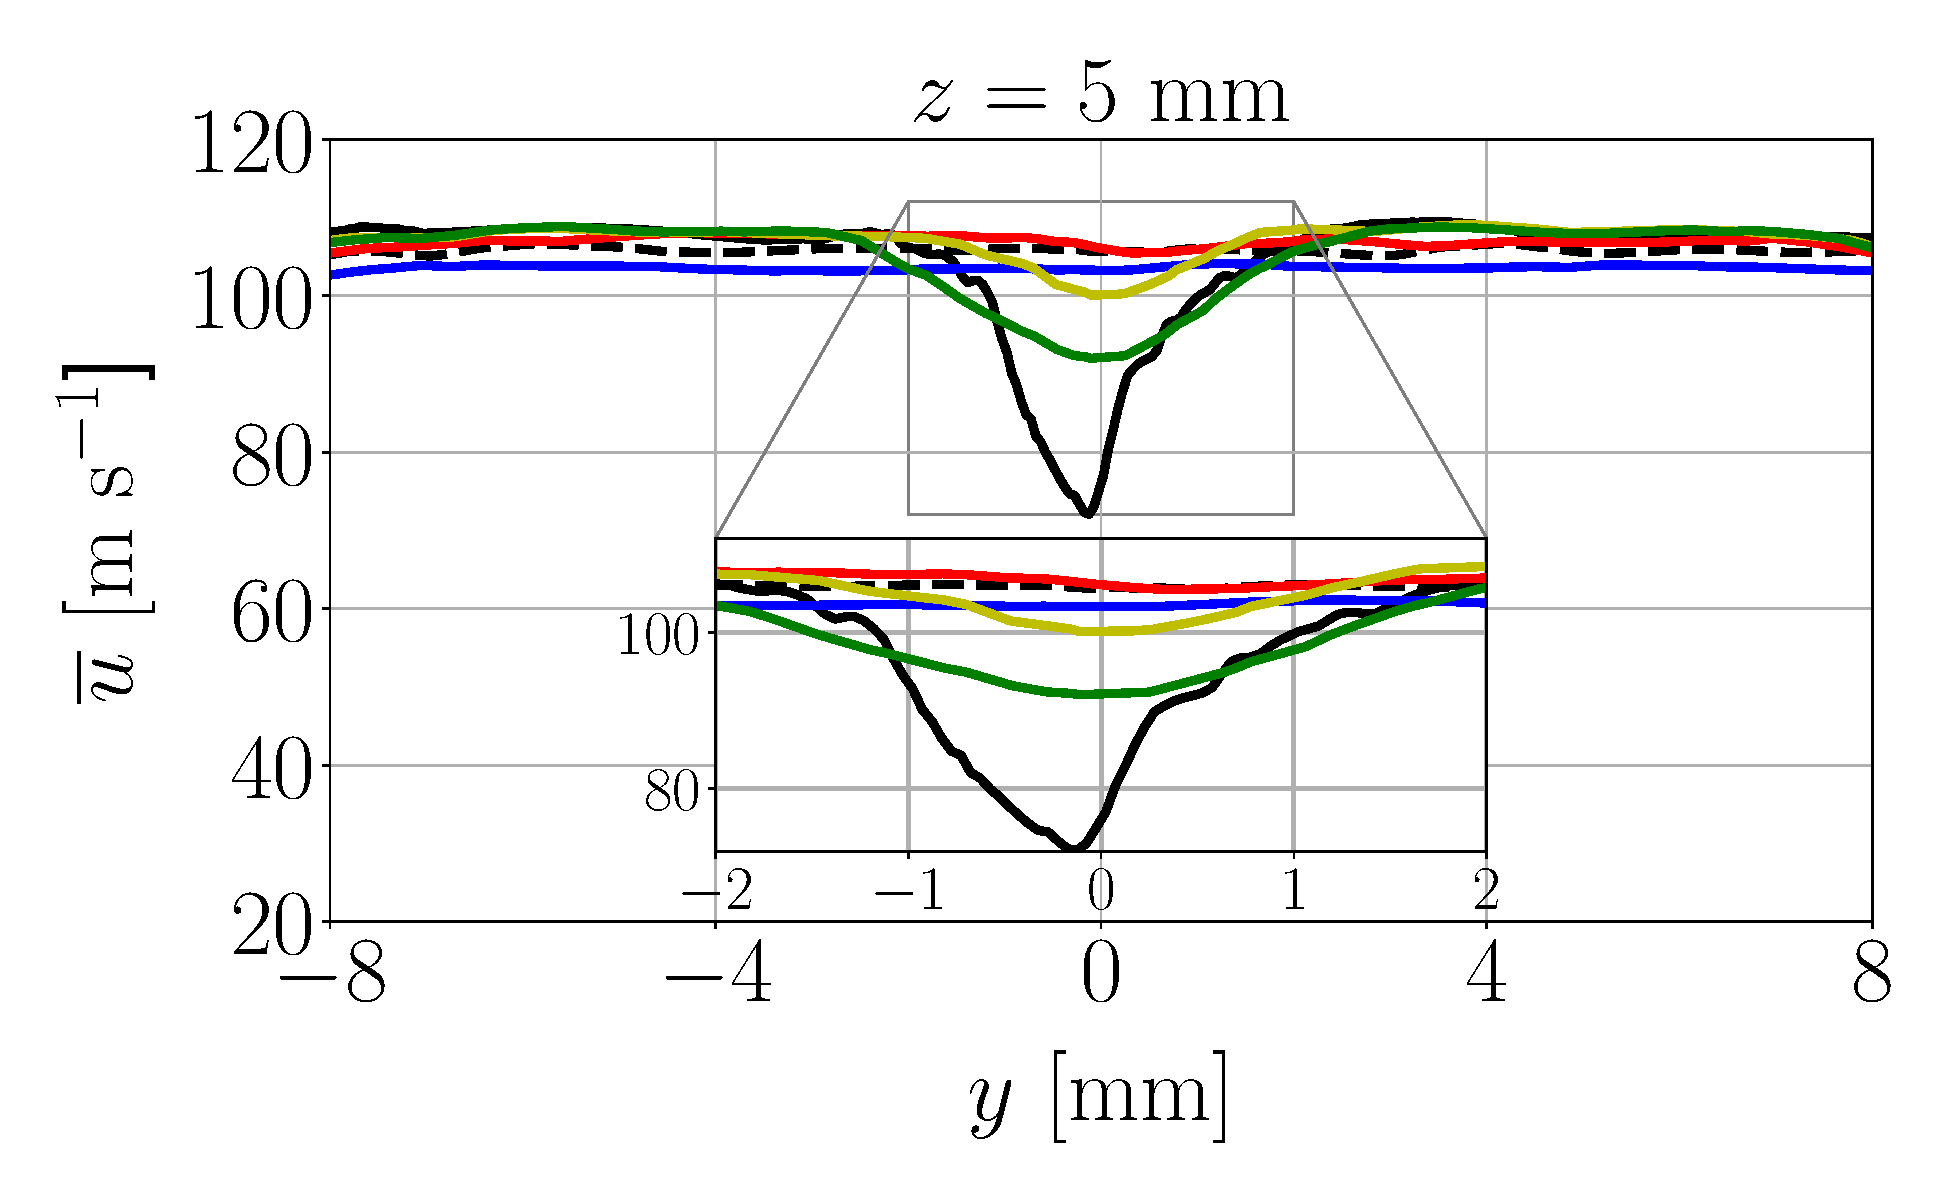
\includegraphics[scale=0.24]{./part2_developments/figures_ch6_lagrangian_JICF/gas_field_initial_conditions/ALM_line_x10_z05p0_ux_mean_along_y}
   \vspace*{-0.1in}
	\caption{Plane $x = 10$ mm}
\end{subfigure}
   \caption{Mean axial velocity evolution along lateral coordinate in ALM and resolved simulations at $z$ lines of Figure \ref{fig:ALM_gas_fields_plane_x}}
\label{fig:JICF_ALM_lines_iso-x_along_y_ux_mean}
\end{figure}


In general, it can be concluded that ALM can perturb the gaseous field through the application of body forces. With a simplified geometry, a careful choice for ALM parameters allows to retrieve the main structures of the flow perturbed by a liquid dense core. The parameters directly obtained from the resolved simulations did not yield a realistic disturbed phase, and hence were optimized through trial-and-error. A better methodology to find optimal configuration for ALM could be through a multivariable optimization where the most suitable ALM parameters were found through the minimization of an objective function. Further improvements in the model could also include modifications in the ALM geometry, such as the addition of several actuator models, or the inclusion of frequential effects to better represent the dense core unsteady shape. Such strategies were out of the scope of this thesis and are left for future work. 


\clearpage

\subsubsection*{Prescription of gaseous inlet from resolved simulations }


An alternative strategy to obtain gas boundary conditions is proposed in this section. This one consists of obtaining the gaseous field in a plane perpendicular
to the crossflow from the resolved simulations, and then prescribing this field as the inlet of a reduced computational computational domain. The gaseous field is characterized by the mean and RMS values of the velocities in the three directions. These statistics are then imposed in a reduced domain consisting of a box with length $150$ mm and cross-section 25x40 mm$^2$ representing the downstream part of the plenum from the full JICF configuration. Figure \ref{fig:mesh_reduced_inlet} shows the location of the reduced domain within the geometrical setup from the resolved atomization simulation and the computational grid. The mesh, which contains $12 \cdot 10^6$ elements, has been refined up to a location $x = 40$ mm downstream the inlet to an element size $\Delta x = 0.3$ mm.  Further downstream up to $x = 100$ mm, the cell size has been set to $\Delta x = 0.5$ mm. The finer cell size of $\Delta x = 0.3$ mm has been selected  with the objective of better capturing the turbulent structures created by the inhomogeneous gaseous velocity profile injected. Nevertheless, this cell size is not resolved enough to capture those: in the resolved simulations of Chapter \ref{ch5:jicf_resolved_simulations}, the cell size in the gaseous field around the liquid regions was of the order of the interface cell sizes ($\Delta x_\mathrm{min} = 20, 10~\mu$m), while such resolutions cannot be imposed into this reduced domain as the mesh size would greatly increase, yielding computations more expensive. Furthermore, a too fine mesh would create large volume fractions which are not in accordance with the application of lagrangian methods to simulate dispersed multiphase flows, since they are applicable to small volume fractions \citepColor[murrone_numerical_2011].


\begin{figure}[h!]	
	\centering	
	\includeinkscape[inkscapelatex=false,scale=0.25]{./part2_developments/figures_ch6_lagrangian_JICF/mesh_reduced_inlet}
	\caption{Location of the reduced domain within the resolved atomization computational setup (in green) and mesh details}
	\label{fig:mesh_reduced_inlet}
\end{figure}






The methodology to obtain and prescribe gaseous boundary conditions in the reduced domain is illustrated in Figure \ref{fig:custom_inlet_methodology}. Mean and RMS velocity profiles are extracted from the resolved atomization in a plane perpendicular to the crossflow. Then, velocity in the truncated setup is prescribed through the following law:

\begin{equation}
\label{eq:prescribed_inlet_u_gas_injection_law}
\textbf{u} \left( \textbf{x}, t \right) = \overline{\textbf{u}} \left( \textbf{x} \right)  + r \left( t \right)  \textbf{u}_\mathrm{RMS} \left( \textbf{x} \right) 
\end{equation}

where $\overline{\textbf{u}} \left( \textbf{x} \right)$ and $\textbf{u}_\mathrm{RMS} \left( \textbf{x} \right)$ are the mean and RMS velocity distributions. $r \left( t \right)$ is a time-varying scalar sampled from a normal distribution with mean 0 and variance 1: $r \sim \mathcal{N} \left( \mu = 0, \sigma^2 = 1 \right)$. This velocity prescription law, which is based on the weak recycling method of synthetic turbulence injection by \citeColor[wu_large_1995], ensures that the injected $TKE$ in the dispersed phase simulations is the same as the one retrieved from the resolved atomization ones. Hereafter, this methodology will be referred as \textbf{prescribed gaseous inlet}.

%\hl{Nevertheless, due to the coarser mesh employed in the reduced domain with respect to the }

\clearpage

\begin{figure}[h!]	
	\centering	\includeinkscape[inkscapelatex=false,scale=0.25]{./part2_developments/figures_ch6_lagrangian_JICF/gas_field_initial_conditions/custom_inlet_methodology}
	\caption{Methodology to prescribe mean and RMS velocity fields from resolved simulations in reduced domain for dispersed-phase computation.}
	\label{fig:custom_inlet_methodology}
\end{figure}


%\subsubsection{Setup and results}

The injected in-plane profiles have been obtained at the location $x = 3$ mm downstream the liquid injection nozzle in the resolved atomization simulations. Other plane locations have been tested without observing significant differences in the dispersed-phase simulations. In fact, the range of the possible planes to retrieve gaseous data for prescribing inlet BCs is narrow: upstream $x = 3$ mm the jet dense core is present and mean gaseous profiles would contain velocities corresponding to the liquid phase, while further downstream the lagrangian spray is injected in the dispersed-phase simulations (the earliest injection location is $x = 5$ mm). Hence, the only reported case hereafter corresponds to the location $x = 3$ mm. Since the computational domain is reduced with respect to the full computational configuration, the axial coordinates are shifted by 3 mm and the experimental validation plane, located at 80 mm downstream the liquid injection nozzle in the test bench, correspond indeed to the location $x = 77$ mm. From now on, however, all axial coordinates reported will be expressed in the absolute reference frame of the experimental test bench for easing comparison with the ALM dispersed-phase simulations. 

Figure \ref{fig:custom_gas_fields_plane_Y} shows results for the mean axial velocity at plane $y = 0$ mm. Statistics from the resolved case UG100\_DX10 have been used in the reduced domain. Both the resolved atomization simulation and the prescribed gaseous simulation are shown: the former shows the field up to the location $x = 3$ mm (prescription plane), then the gaseous field corresponds to the prescribed gaseous inlet. The velocity field shows good continuity among simulations at the prescription plane, indicating that the resolved field is correctly specified in the gaseous simulation. The perturbation created by the prescribed simulation is very close to the resolved simulation at vertical locations $z < 4$ mm, as shown by the profiles along the white lines plotted in Figures \ref{fig:JICF_ICS_custom_lines_y0_along_x_ux_mean} and \ref{fig:JICF_ICS_custom_lines_y0_along_z_ux_mean}. For locations further from the wall ($z > 4$ mm), velocities in the prescribed deviates from the profiles of the resolved one, indeed approaching the velocities from the optimal ALM simulation. In the resolved simulations, perturbations far away from the wall are created by ligaments ejected from the dense core, which can be present up to several diameters downstream the liquid nozzle (see for instance Figure \ref{fig:jicf_sps_with_gaseous_planes}, where ligaments are found up to $x = 5$ mm). In the prescribed simulation, gaseous statistics are specified at $x = 3$ mm and there is no liquid present to perturb the gaseous field as ligaments do in the resolved simulations, hence such disturbances are not captured. As commented before, changing the location of the gaseous inlet at further upstream or downstream (prior to $x = 5$ mm, since lagrangian droplets will be injected at this location) had no influence on the gaseous field.

\begin{figure}[h!]	
	\centering	\includeinkscape[inkscapelatex=false,scale=0.30]{./part2_developments/figures_ch6_lagrangian_JICF/gas_field_initial_conditions/custom_inlet_planes_y}
	\caption[Mean axial velocity field at plane $y = 0$ for resolved case UG100\_DX10 and prescribed gaseous inlet]{Mean axial velocity field at plane $y = 0$ for resolved case UG100\_DX10 and prescribed gaseous inlet. The resolved simulation is cut at $x = 3$ mm, location from which the prescribed gaseous inlet simulation starts. Both computations are independent and are shown simultaneously in this figure for visual comparison of the flow fields}
	\label{fig:custom_gas_fields_plane_Y}
\end{figure}

\begin{figure}[ht]
\flushleft
\begin{subfigure}[b]{0.45\textwidth}
	\centering
   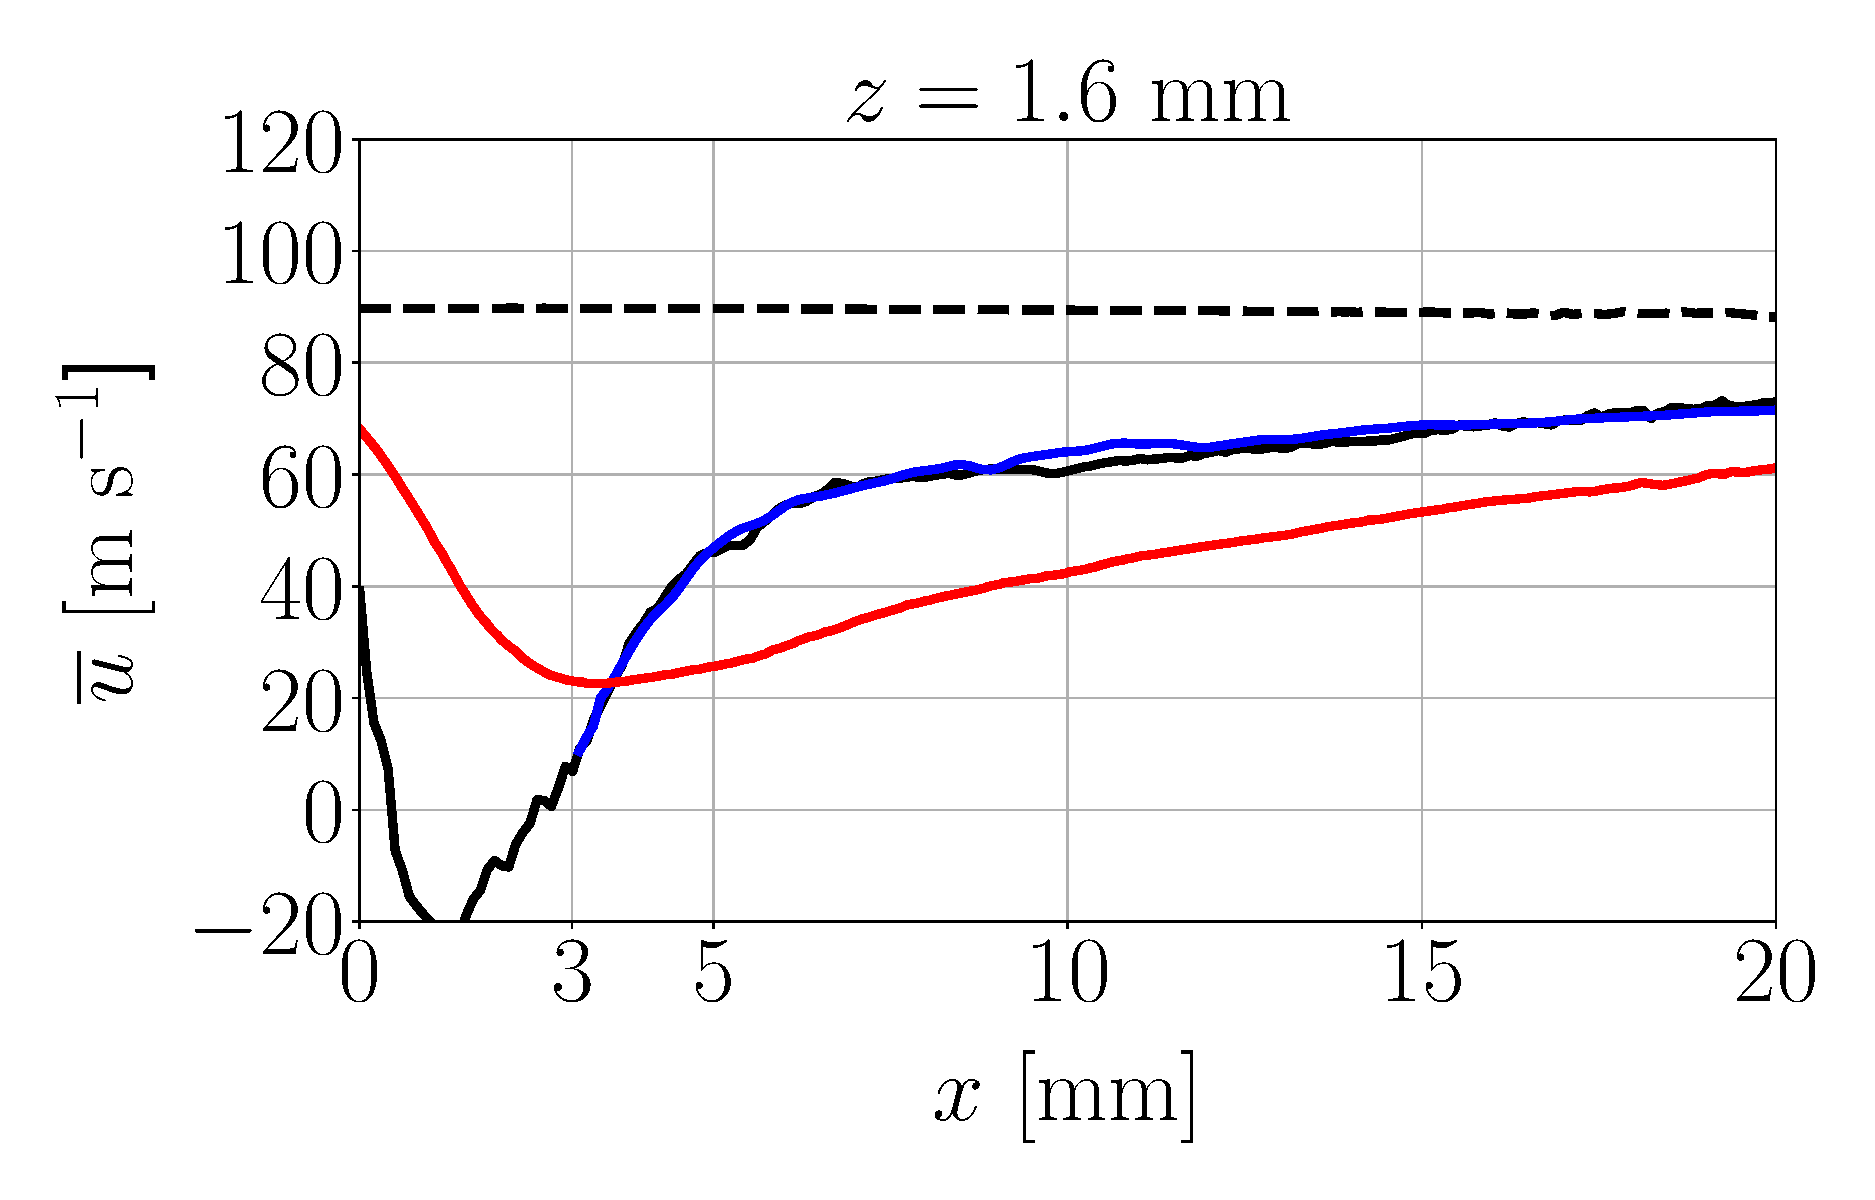
\includegraphics[scale=0.25]{./part2_developments/figures_ch6_lagrangian_JICF/gas_field_initial_conditions/custom_line_y0_along_x_z01p6}
   %\caption{}
   %\label{} 
\end{subfigure}
\hspace{0.4in}
\begin{subfigure}[b]{0.45\textwidth}
	\centering
   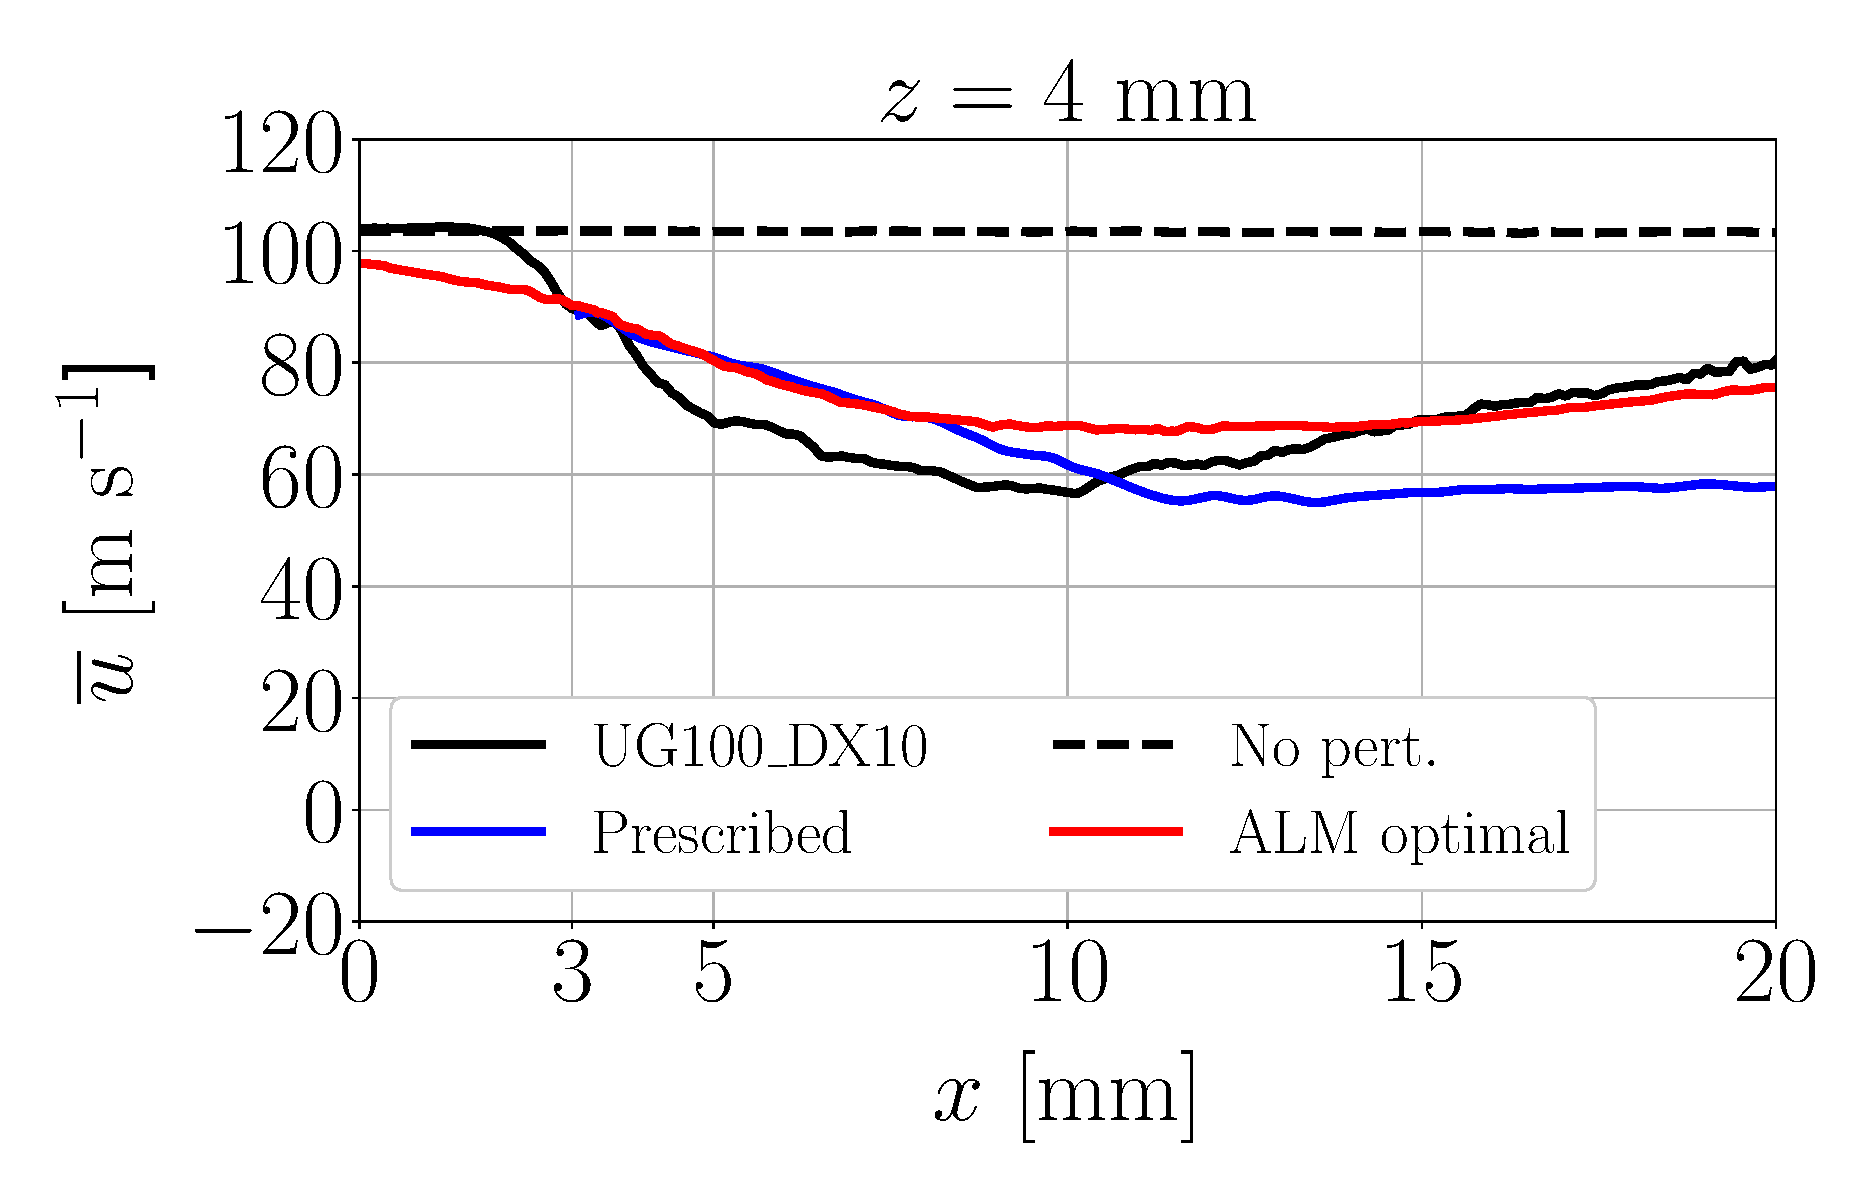
\includegraphics[scale=0.25]{./part2_developments/figures_ch6_lagrangian_JICF/gas_field_initial_conditions/custom_line_y0_along_x_z04p0}
   %\caption{}
   %\label{}
\end{subfigure}
\caption{Mean axial velocity evolution along axial coordinate at locations $z = 1.6, 4$ mm in plane $y = 0$}
\label{fig:JICF_ICS_custom_lines_y0_along_x_ux_mean}
\end{figure}

\begin{figure}[ht]
\centering
   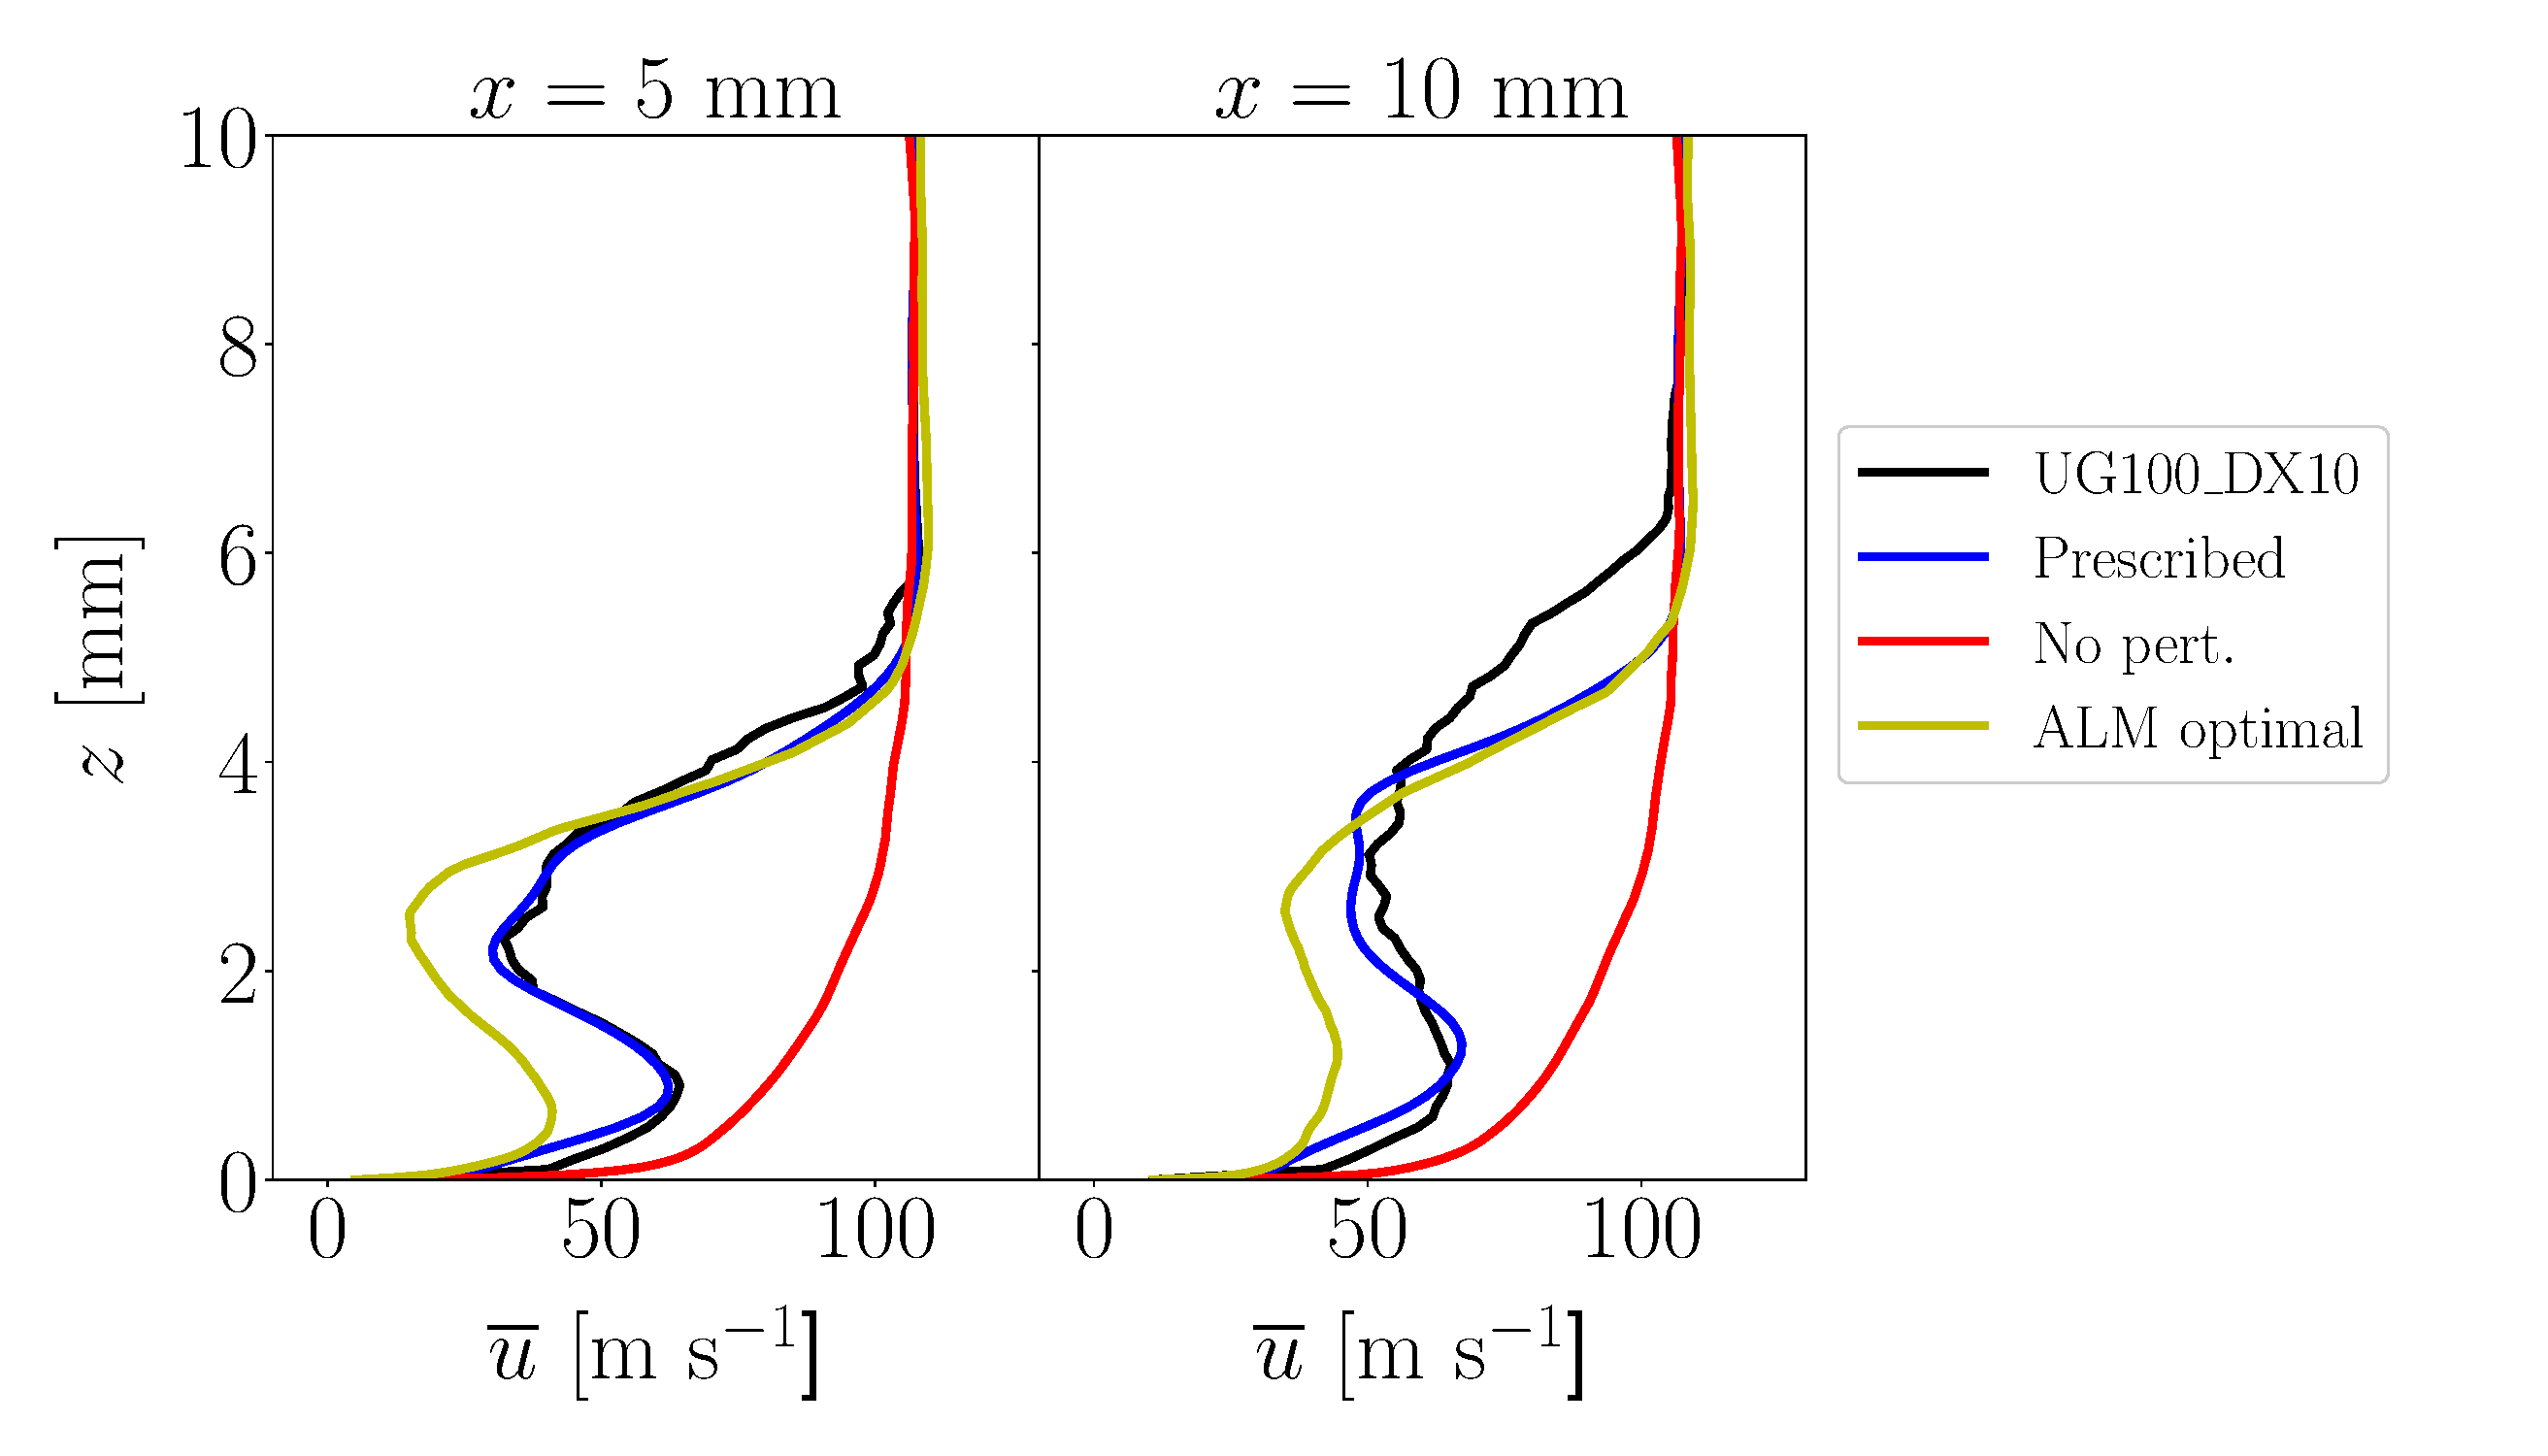
\includegraphics[scale=0.26]{./part2_developments/figures_ch6_lagrangian_JICF/gas_field_initial_conditions/custom_lines_y0_along_z_ux_mean}
\caption{Mean axial velocity evolution along vertical coordinate at $x = 2.5, 5, 10$ mm locations of plane $y = 0$ (lines of Figure \ref{fig:custom_gas_fields_plane_x}) }
\label{fig:JICF_ICS_custom_lines_y0_along_z_ux_mean}
\end{figure}
\clearpage

The flow field at planes perpendicular to crossflow direction $x = 5, 10$ mm  are displayed in Figure \ref{fig:custom_gas_fields_plane_x}. The prescribed gaseous inlet can retrieve the Counter-Rotating Vortices (CRVs) spinning directions in both cases. At $x = 5$ mm the vertical location of the CRV is underestimated with respect to the resolved case, while further downstream it gets closer. The velocity profiles along the white lines are shown in Figure \ref{fig:JICF_custom_lines_iso-x_along_y_ux_mean}.  Closer to the wall ($z = 1.6$ mm), the prescribed inlet profile coincides with the resolved one in all the range except for the local minima captured at both sides close to $y = 0$, which are not present in the resolved case. Further from the wall ($z = 5$ mm) the prescribed profile does not match the resolved profile due to the reasons aforementioned, and creates flow decelerations with magnitudes similar to the ALM optimal case. 

\begin{figure}[h!]	
	\centering	\includeinkscape[inkscapelatex=false,scale=0.265]{./part2_developments/figures_ch6_lagrangian_JICF/gas_field_initial_conditions/custom_inlet_planes_x}
	\caption{Mean axial velocity field at planes $x = 5, 10$ mm for resolved case UG100\_DX10 and prescribed gaseous inlet}
	\label{fig:custom_gas_fields_plane_x}
\end{figure}

\begin{figure}[ht]
\centering
\begin{subfigure}[b]{1.0\textwidth}
	\centering
   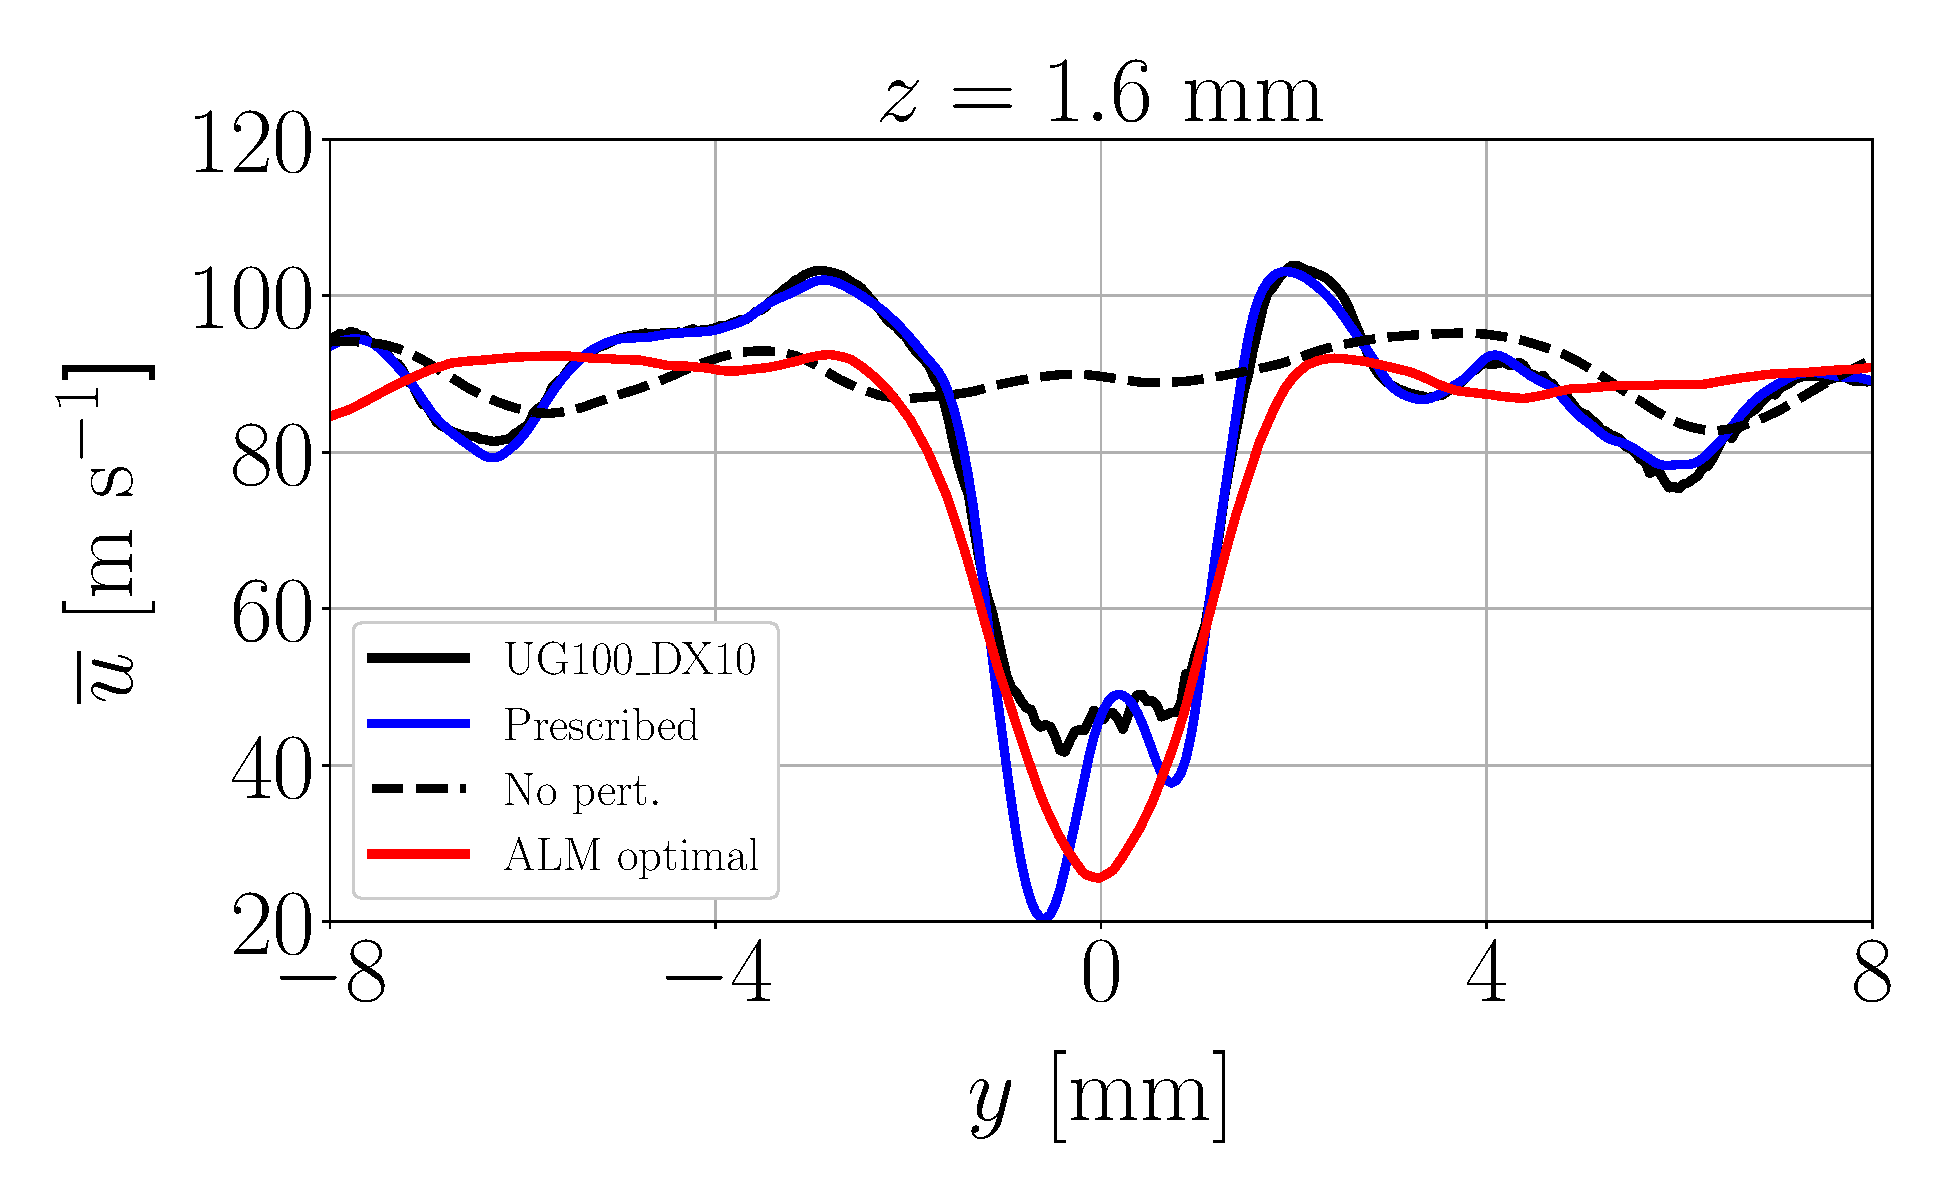
\includegraphics[scale=0.24]{./part2_developments/figures_ch6_lagrangian_JICF/gas_field_initial_conditions/custom_line_x05_z01p6_ux_mean_along_y}
   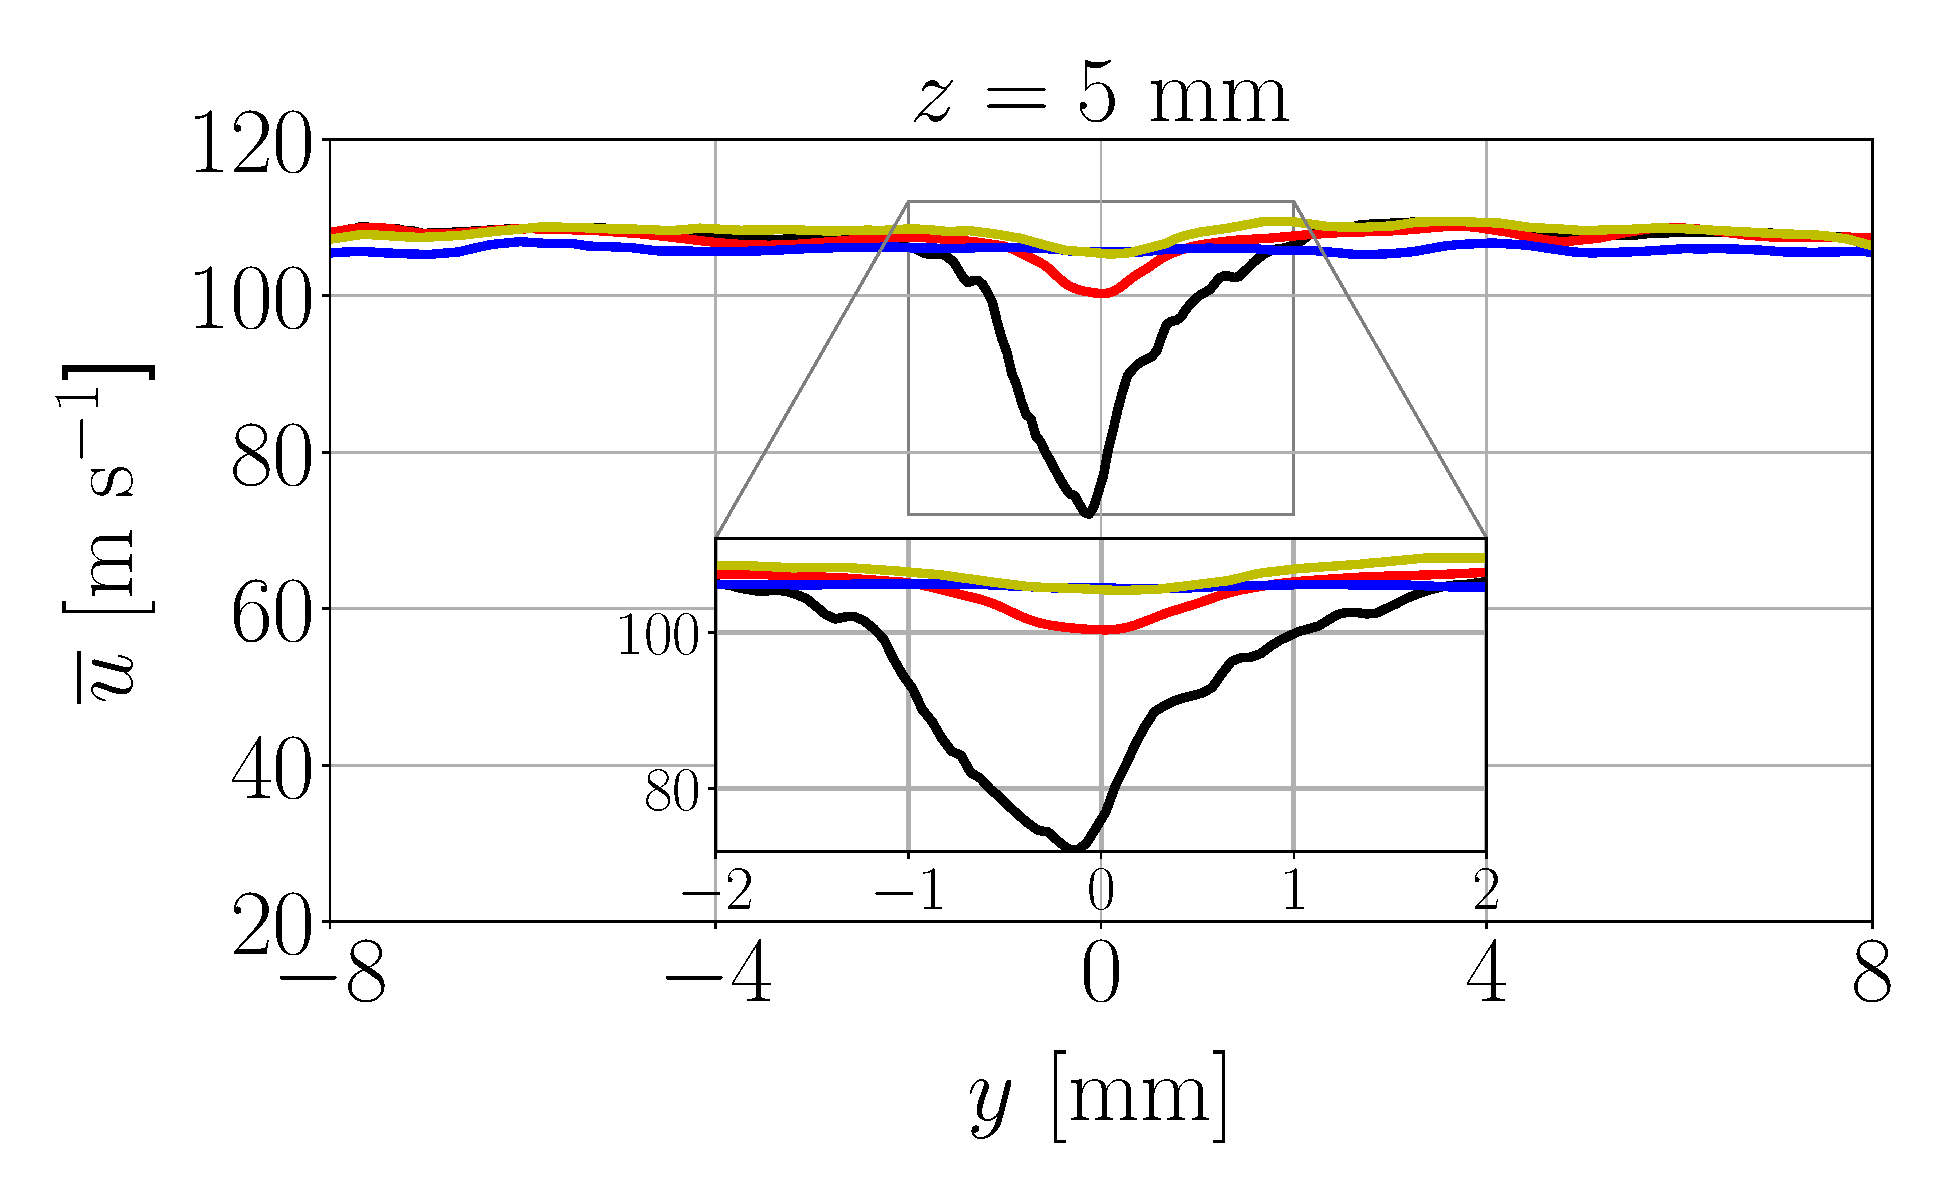
\includegraphics[scale=0.24]{./part2_developments/figures_ch6_lagrangian_JICF/gas_field_initial_conditions/custom_line_x05_z05p0_ux_mean_along_y}
   \vspace*{-0.1in}
	\caption{Plane $x = 5$ mm}
\end{subfigure}
\vskip\baselineskip
\begin{subfigure}[b]{1.0\textwidth}
	\centering
   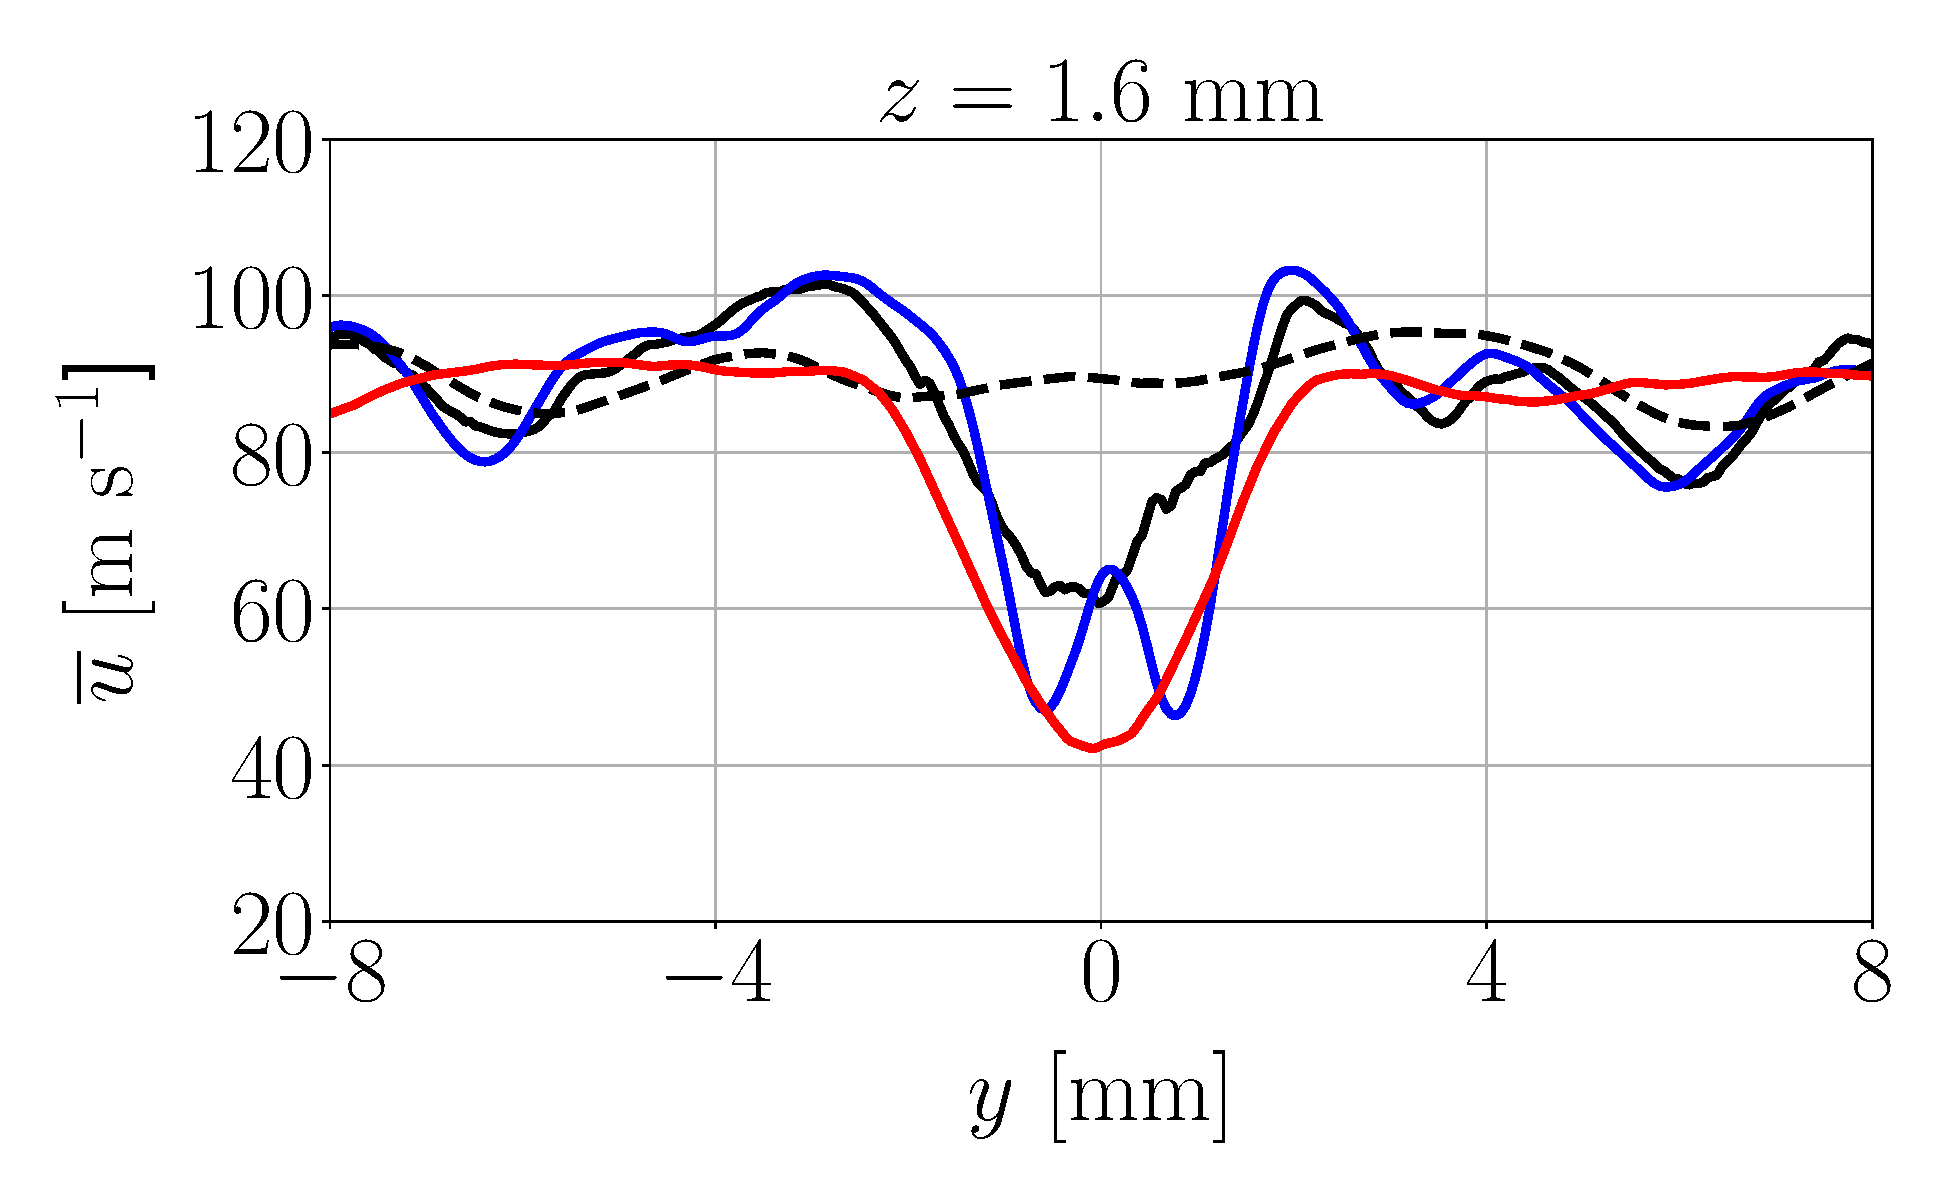
\includegraphics[scale=0.24]{./part2_developments/figures_ch6_lagrangian_JICF/gas_field_initial_conditions/custom_line_x10_z01p6_ux_mean_along_y}
   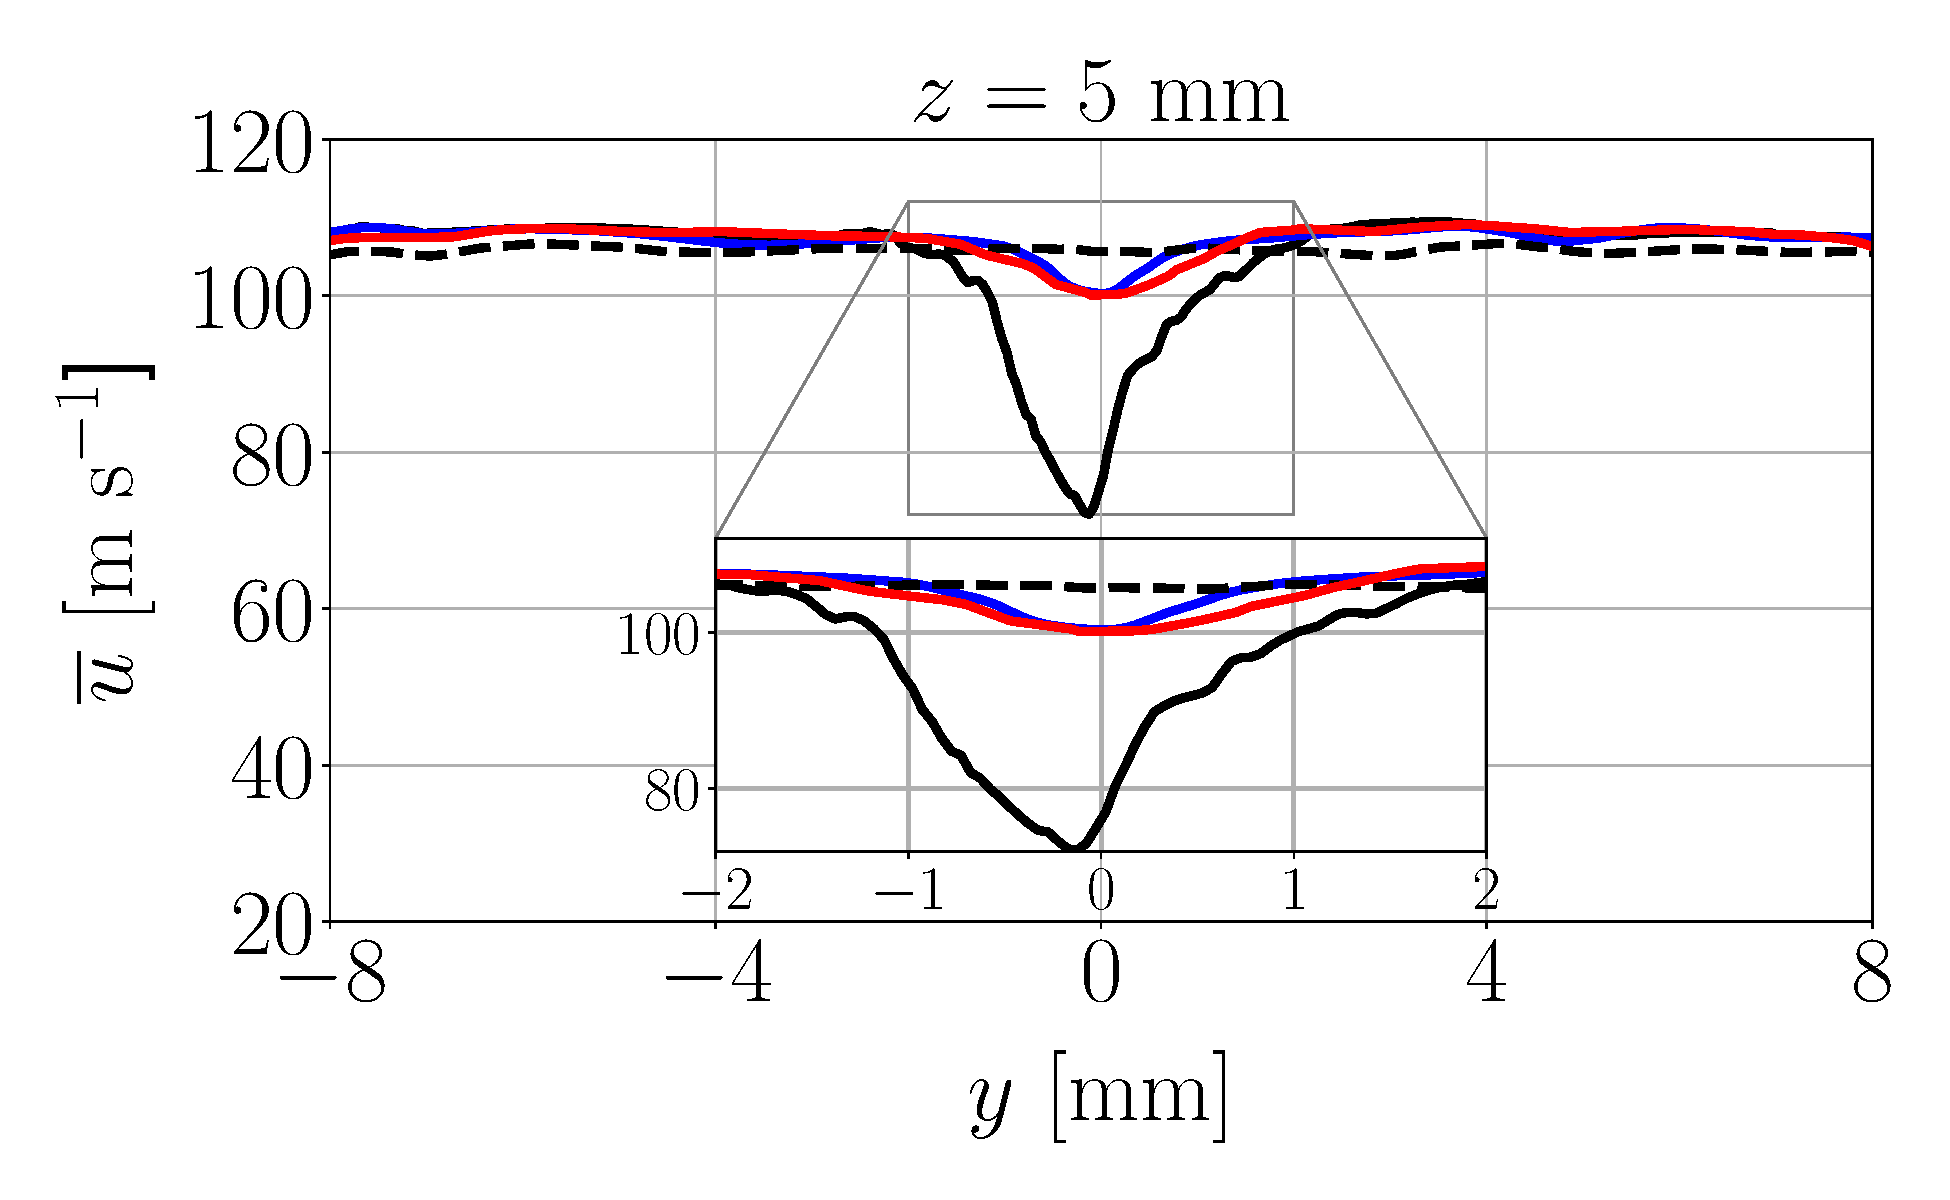
\includegraphics[scale=0.24]{./part2_developments/figures_ch6_lagrangian_JICF/gas_field_initial_conditions/custom_line_x10_z05p0_ux_mean_along_y}
   \vspace*{-0.1in}
	\caption{Plane $x = 10$ mm}
\end{subfigure}
   \caption{Mean axial velocity evolution along lateral coordinate at $z$ lines of Figure \ref{fig:custom_gas_fields_plane_x}}
\label{fig:JICF_custom_lines_iso-x_along_y_ux_mean}
\end{figure}

It can be concluded that the prescribed inlet captures more accurately the gaseous field than the ALM tested. Furthermore, its computational cost is lower, since the reduced domain represents only a fraction of the original computational setup and less mesh elements are used. On the contrary, its main disadvantage a priori is its only applitability to simple geometries such as the academic JICF tested. 



\subsection{Lagrangian jet establishment}

The previous gaseous fields are now taken as initial solutions to perform dispersed-phase computations. To initialize the SLI, the injectors used correspond to the resolved simulation UG100\_DX10 obtained at $x = 5$ mm are used to prescribed liquid boundary conditions. These are shown in Figure \ref{fig:maps_SLI_with_RMS}. Injected mean velocities are Volume-Weighted (VW) within each sampling probe according to Eq. (\ref{eq:ch4_f_arbitrary_mean_RMS_VW_definition}). The RMS components of the velocities are also considered. The injected velocity $\textbf{u}_\mathrm{inj}$ is the prescribed by the expression $\textbf{u}_\mathrm{inj} = \textbf{u}_\mathrm{VW} + r \textbf{u}_\mathrm{RMS,VW}$, where $r$ is a random number sampled from a Gaussian distribution (more details on velocity prescription are given in $S$\ref{subsec:ch4_injectors_definition}).



\begin{figure}[h!]
\flushleft
\begin{subfigure}[b]{0.2\textwidth}
	\flushleft
	\hspace*{-0.45in}
   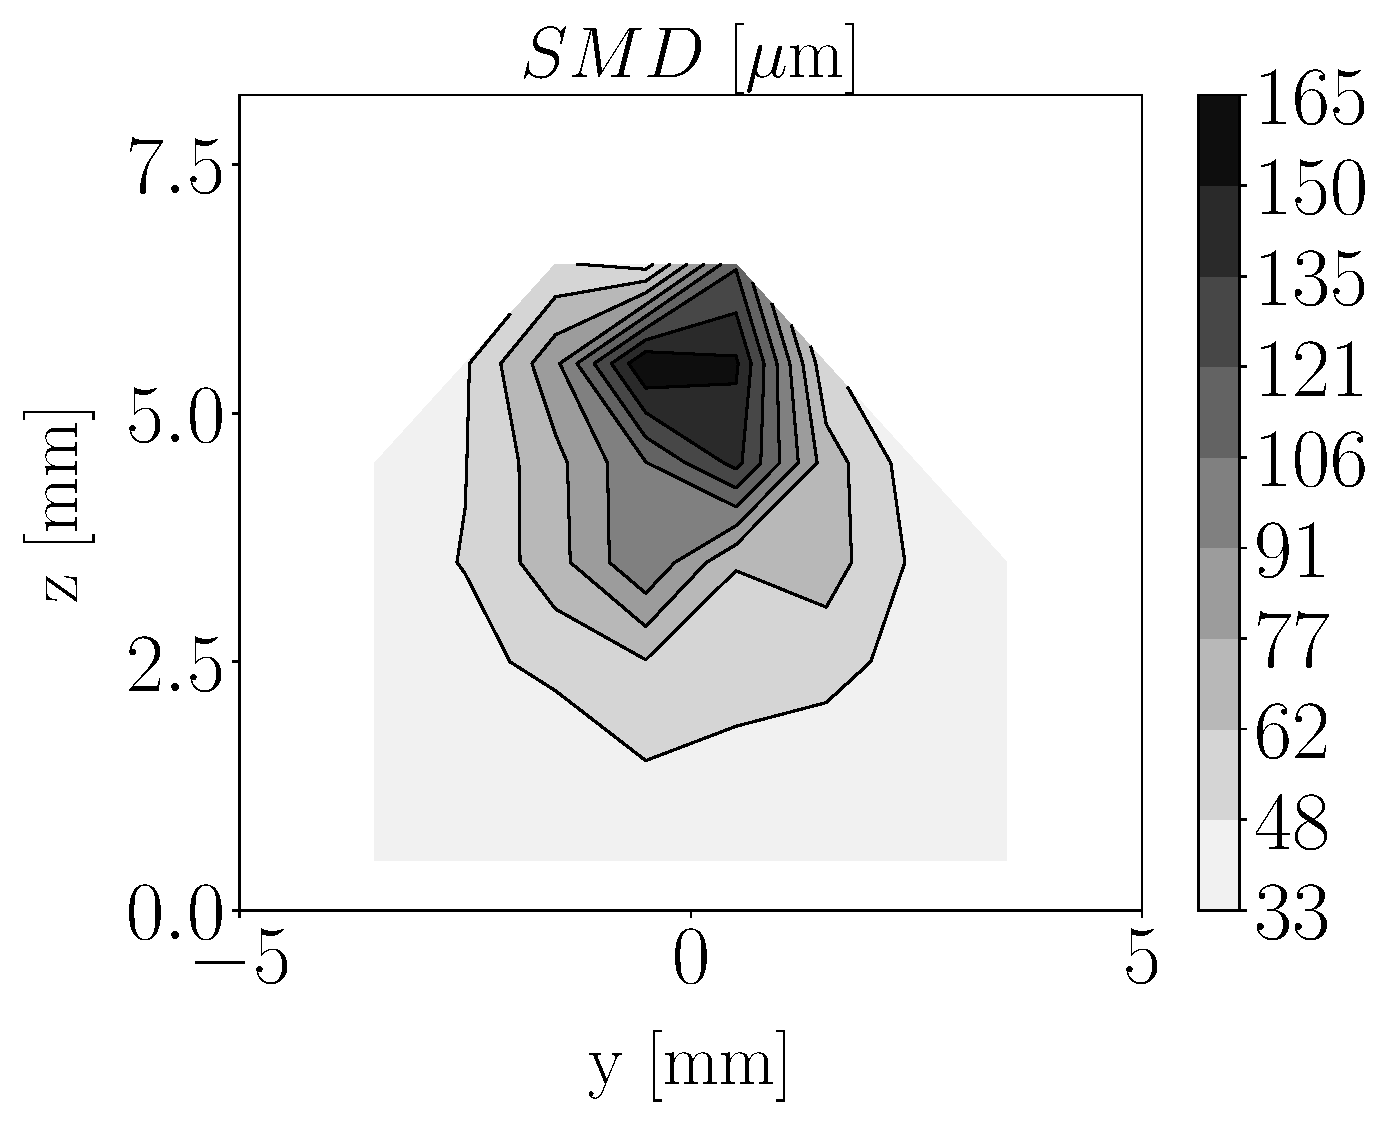
\includegraphics[scale=0.19]{./part2_developments/figures_ch6_lagrangian_JICF/injectors_SLI/uG100_dx10_x05_SMD_map}
   %\label{} 
\end{subfigure}
\hspace*{0.075in}
\begin{subfigure}[b]{0.2\textwidth}
	\flushleft
   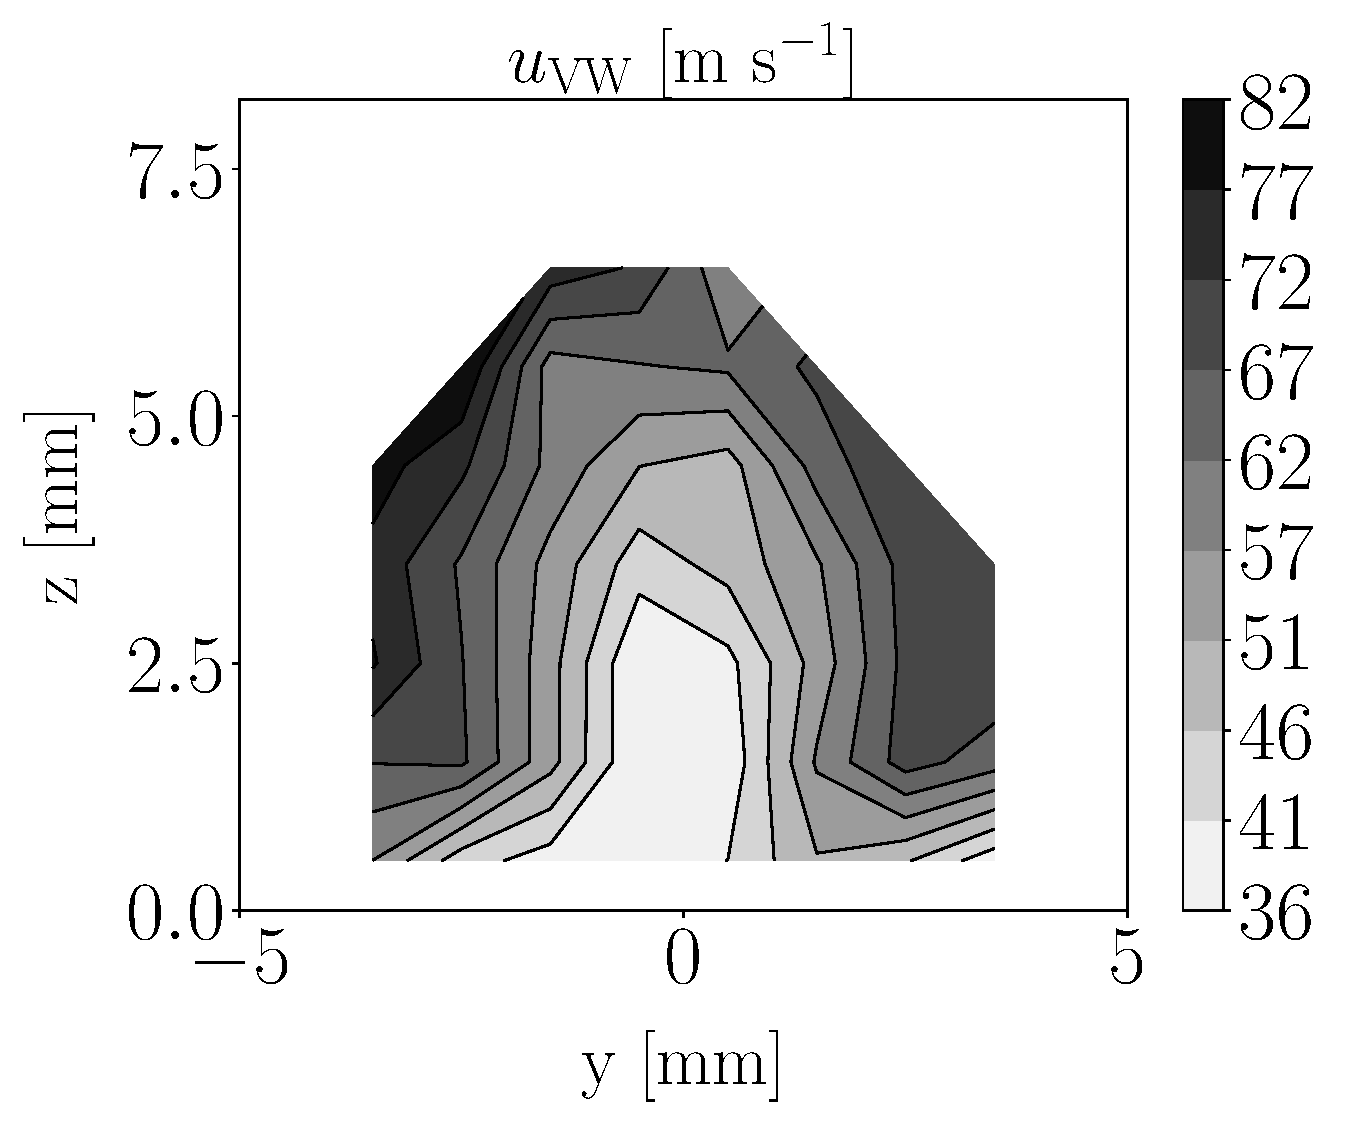
\includegraphics[scale=0.19]{./part2_developments/figures_ch6_lagrangian_JICF/injectors_SLI/uG100_dx10_x05_ux_mean_vw_map}
   %\label{} 
\end{subfigure}
\hspace*{0.45in}
\begin{subfigure}[b]{0.2\textwidth}
	\flushleft
   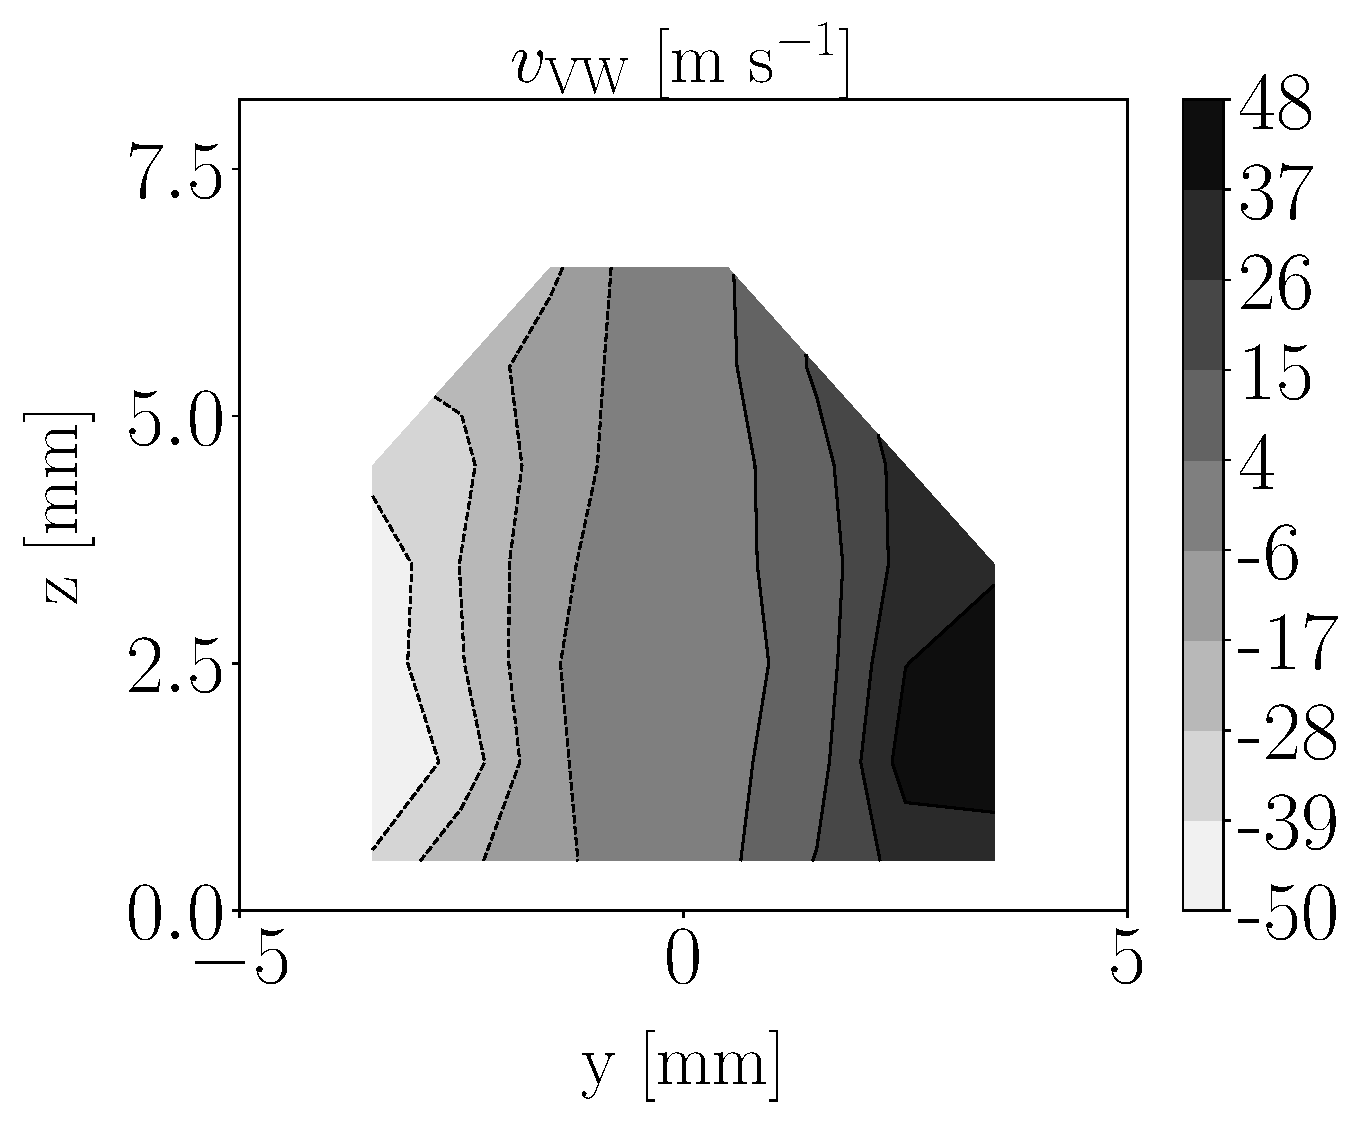
\includegraphics[scale=0.19]{./part2_developments/figures_ch6_lagrangian_JICF/injectors_SLI/uG100_dx10_x05_uy_mean_vw_map}
   %\label{} 
\end{subfigure}
\hspace*{0.45in}
\begin{subfigure}[b]{0.2\textwidth}
	\flushleft
   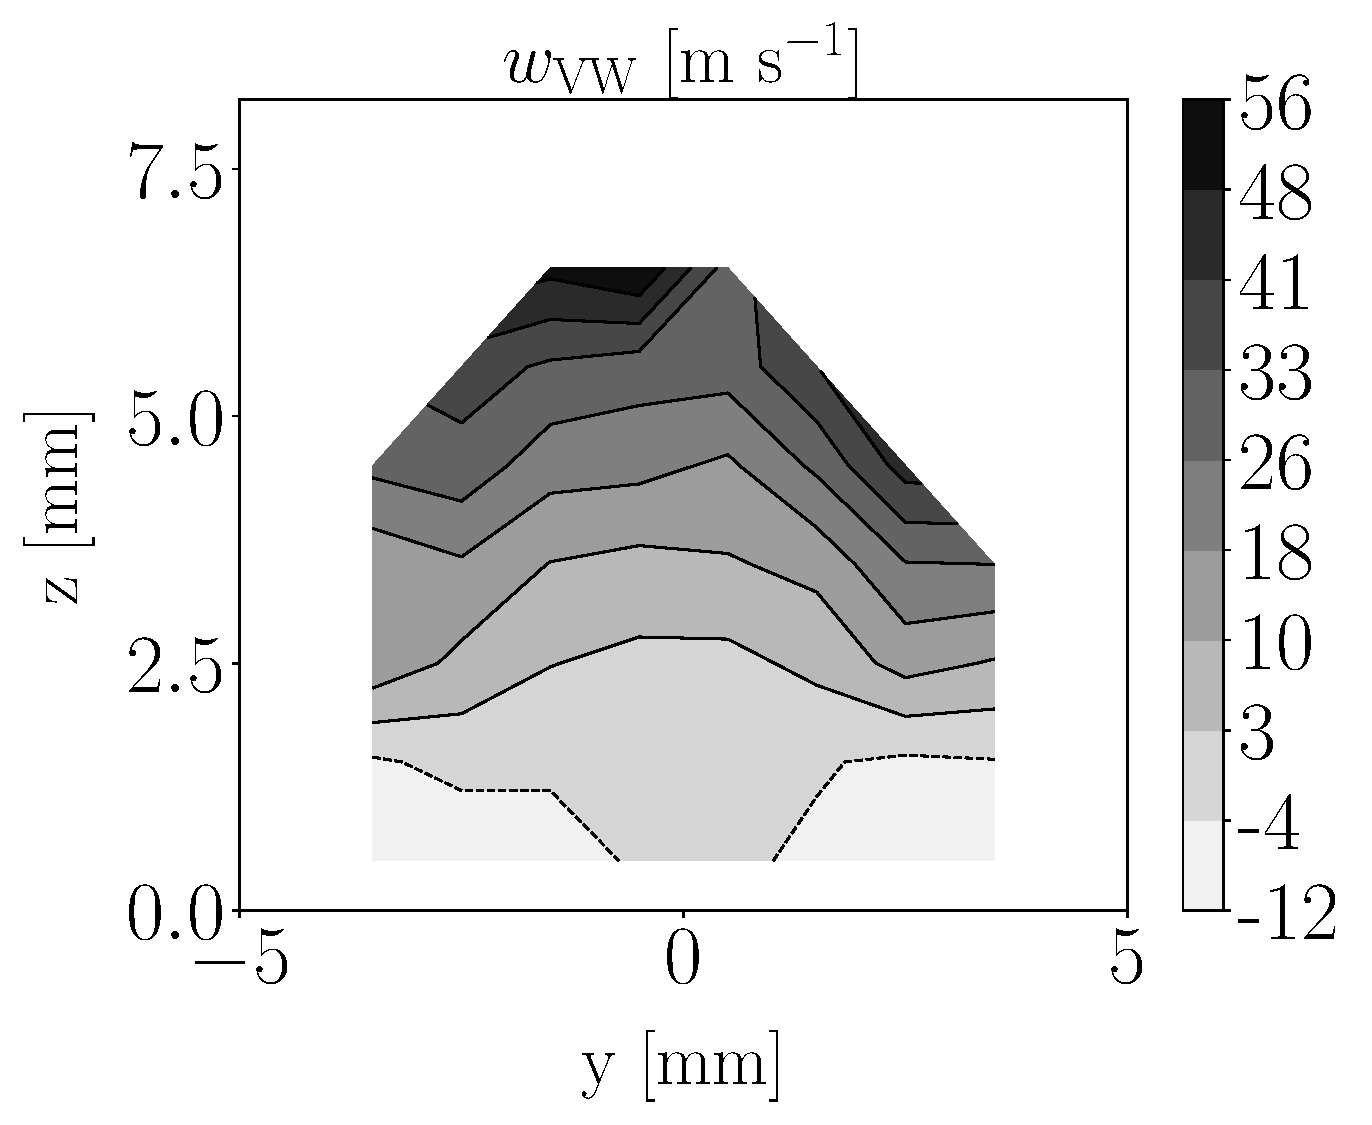
\includegraphics[scale=0.19]{./part2_developments/figures_ch6_lagrangian_JICF/injectors_SLI/uG100_dx10_x05_uz_mean_vw_map}
   %\label{} 
\end{subfigure}

\vspace*{-0.20in}

\flushleft
\begin{subfigure}[b]{0.2\textwidth}
	\flushleft
	\hspace*{-0.45in}
   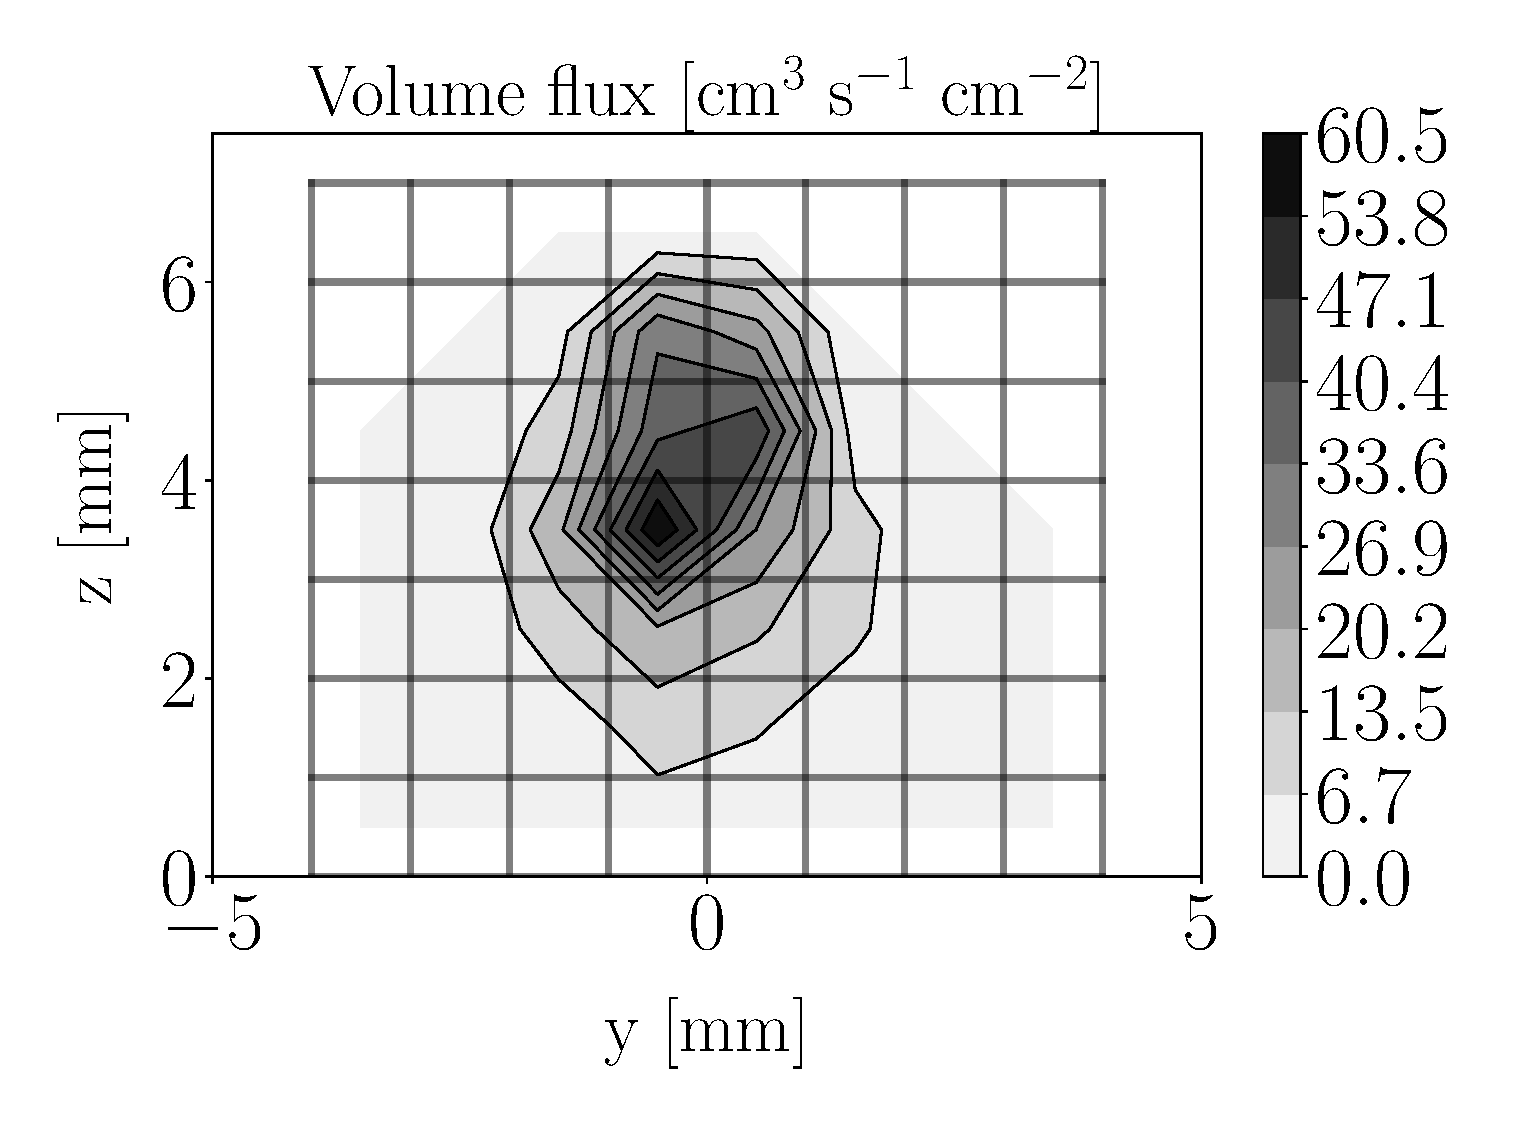
\includegraphics[scale=0.19]{./part2_developments/figures_ch6_lagrangian_JICF/injectors_SLI/uG100_dx10_x05_volume_flux_map}
   %\label{} 
\end{subfigure}
\hspace*{0.075in}
\begin{subfigure}[b]{0.2\textwidth}
	\flushleft
   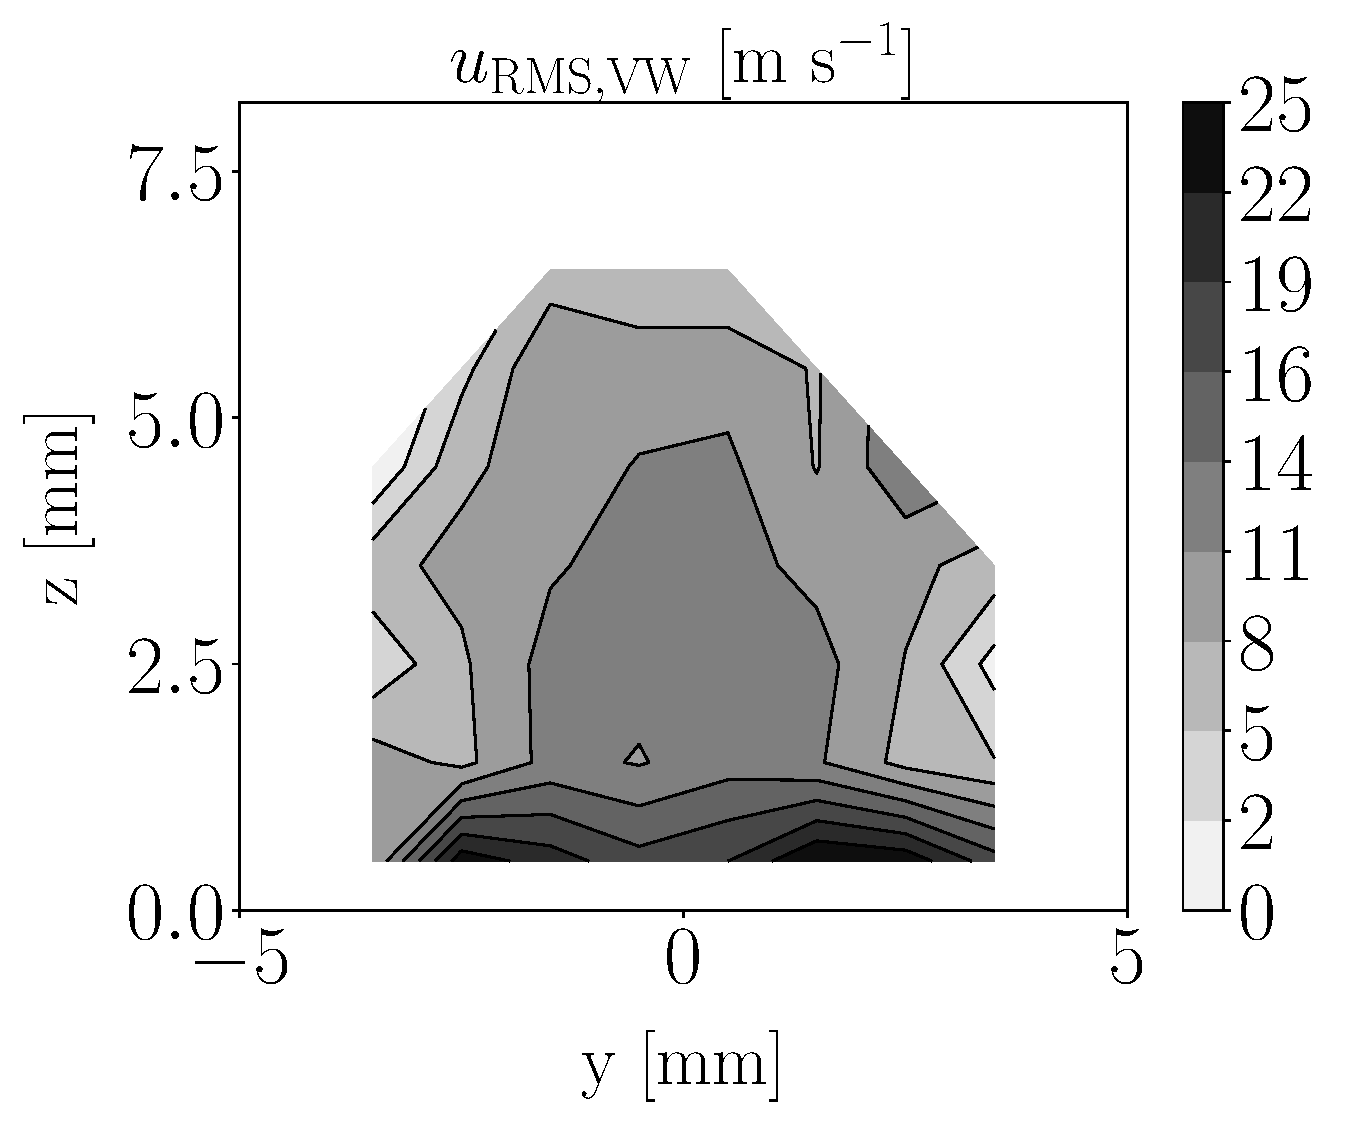
\includegraphics[scale=0.19]{./part2_developments/figures_ch6_lagrangian_JICF/injectors_SLI/uG100_dx10_x05_ux_RMS_vw_map}
   %\label{} 
\end{subfigure}
\hspace*{0.45in}
\begin{subfigure}[b]{0.2\textwidth}
	\flushleft
   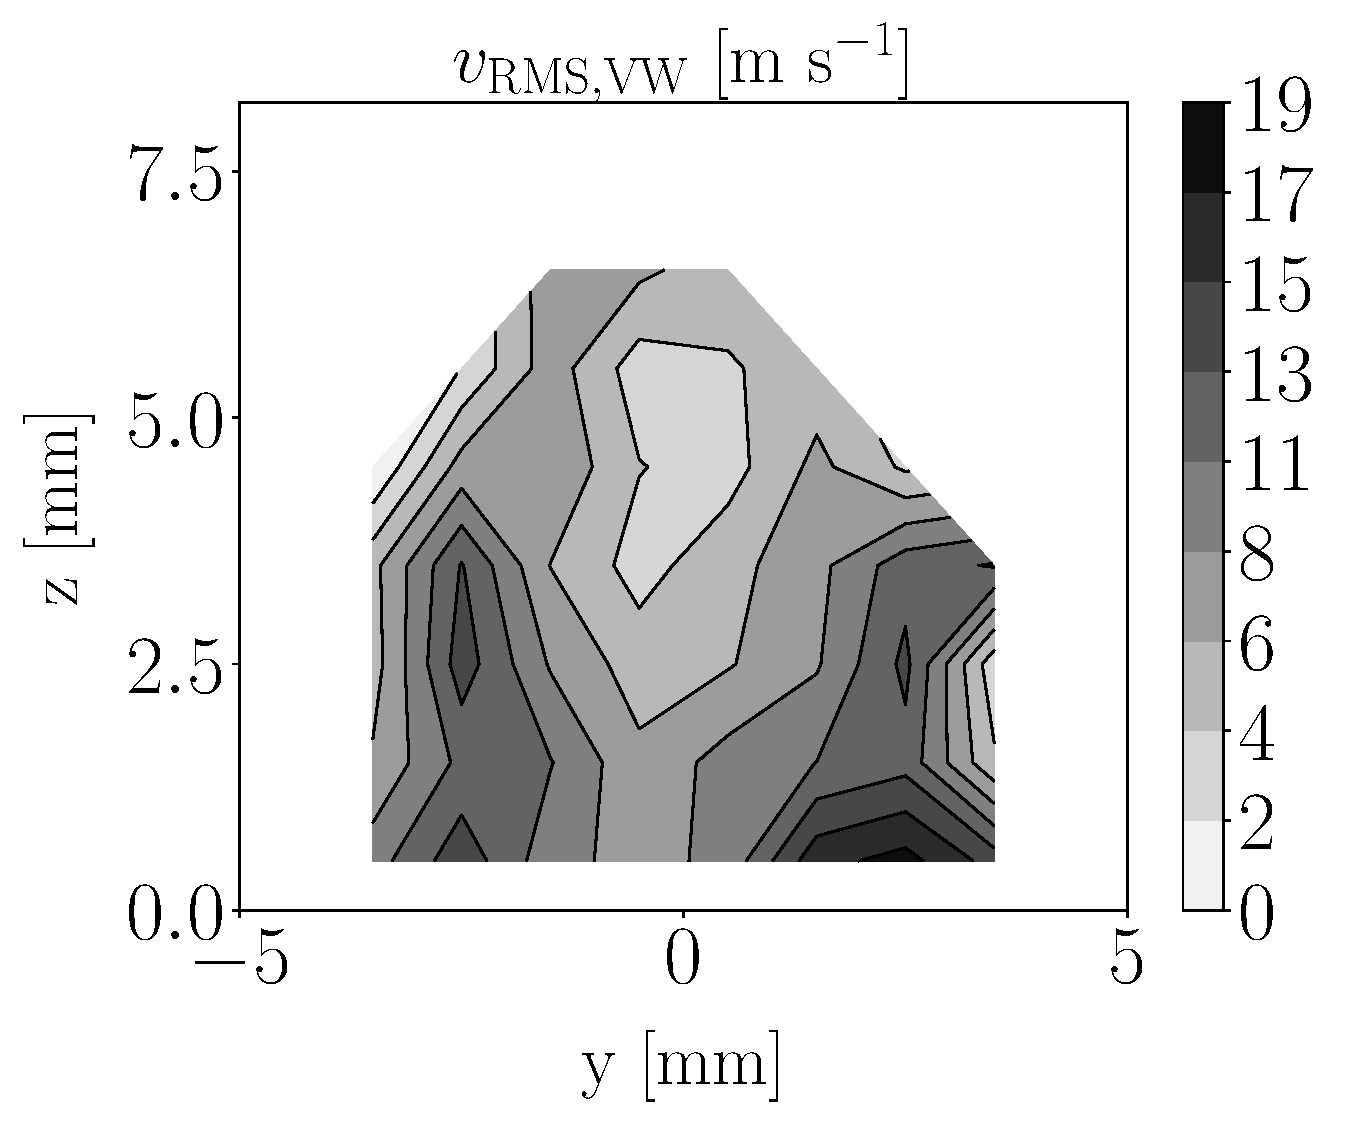
\includegraphics[scale=0.19]{./part2_developments/figures_ch6_lagrangian_JICF/injectors_SLI/uG100_dx10_x05_uy_RMS_vw_map}
   %\label{} 
\end{subfigure}
\hspace*{0.45in}
\begin{subfigure}[b]{0.2\textwidth}
	\flushleft
   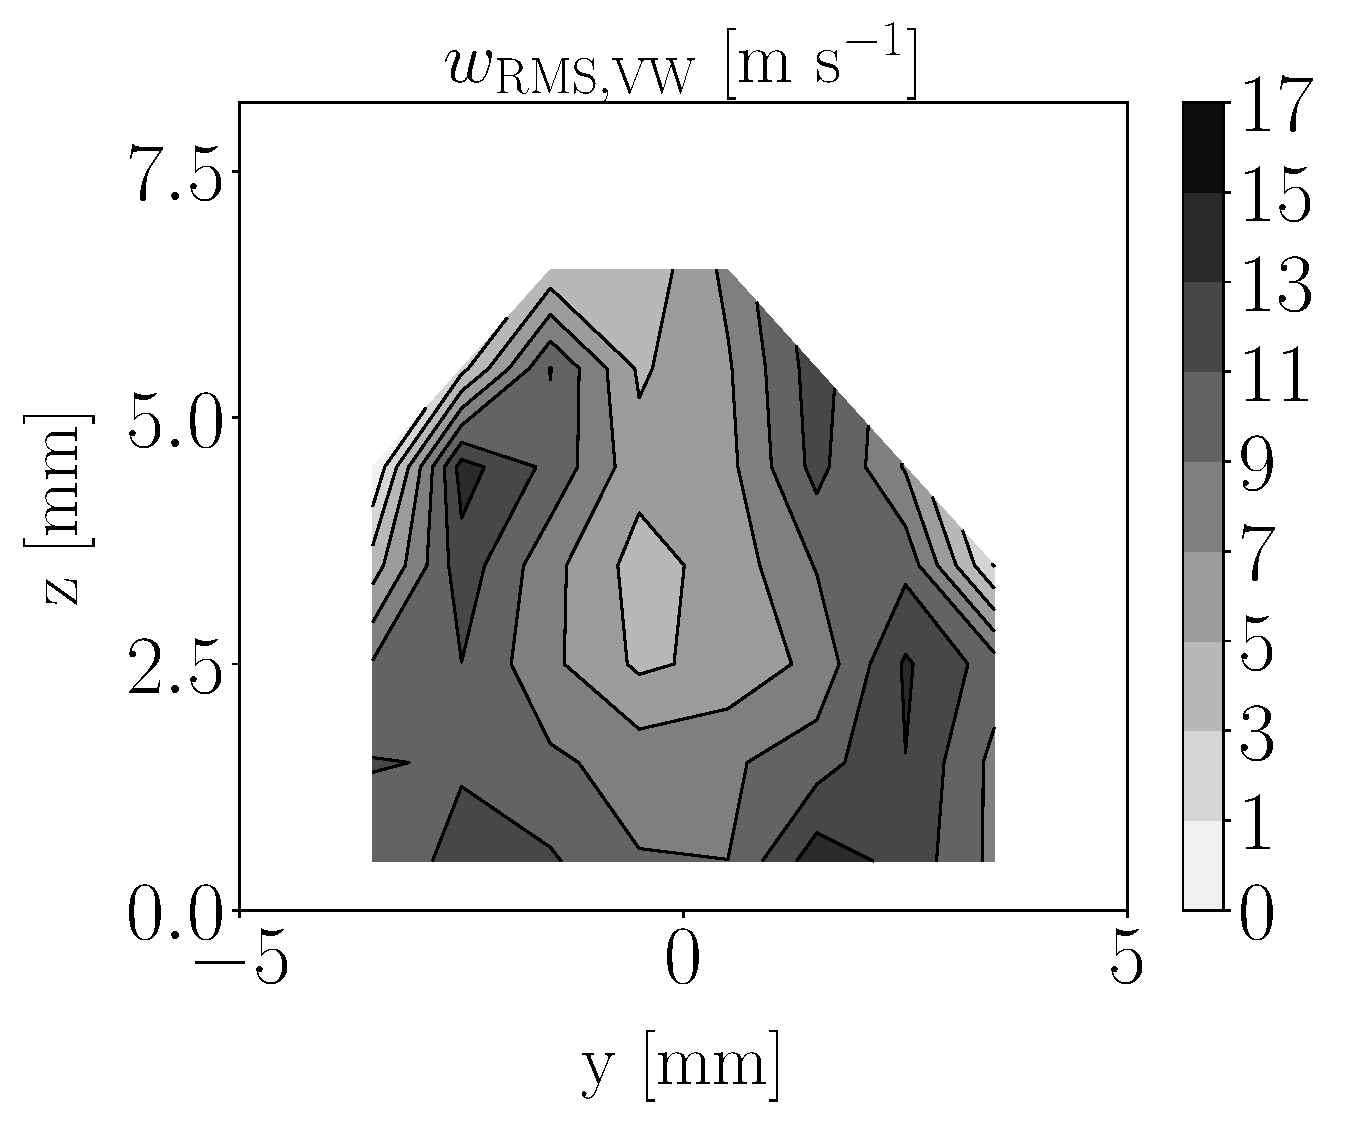
\includegraphics[scale=0.19]{./part2_developments/figures_ch6_lagrangian_JICF/injectors_SLI/uG100_dx10_x05_uz_RMS_vw_map}
   %\label{} 
\end{subfigure}

\caption{SLI mean volume-weighted (VW) and RMS velocity maps from case UG100\_DX10 at $x_\mathrm{inj} = 5$ mm }
\label{fig:maps_SLI_with_RMS}
\end{figure}


The establishment of the dispersed phase for cases ALM optimal and the prescribed inlet are shown in Figure \ref{fig:JICF_LGS_spray_establishment}. In both cases  the injection and experimental validation planes, $x = 5$ and $x = 80$ mm respectively, are shown. The black outline at the first plane denotes the injection region. The prescribed inlet simulation includes as well an instantaneous view of the resolved liquid jet from case UG100\_DX10 solely for visualization among resolved and lagrangian jets: resolved liquid is not actualy present in the dispersed-phase computations. The time instants are expressed in a dimensionless form with respect to the inertial timescale according to Eq. (\ref{eq:t_dimensionless_with_tau_in}).




In both simulations, lagrangian droplets are injected at $x = 5$ mm and then convected downstream. Right after injection, the particles have a finite vertical velocity component which is larger at the spray top than at its bottom.  Consequently, the jet's vertical trajectory continues to increase with axial distance. Shortly after injection, droplets are quickly atomized into smaller particles. The liquid-gas relative velocity is large in all simulations, hence the secondary breakup model triggers atomization soon after injection and the droplets sizes are reduced very fast with axial distance. Indeed, the dispersed-phase simulations show a very abrupt decrease in SMD up to a location between $x = 15$ and $20$ mm, depending on the case. Further downstream, the dispersed spray is fully atomized and droplets are only convected. As a consequence of such a fast breakup, the smaller droplets generated have a lower relaxation time and are quickly dragged by the gaseous crossflow, increasing their axial velocity and reducing their vertical one, hence stopping penetrating in the vertical direction. \clearpage


\begin{figure}[h!]
	\centering	\includeinkscape[inkscapelatex=false,scale=0.8]{./part2_developments/figures_ch6_lagrangian_JICF/jet_establishment/JICF_LGS_establishment}
	\caption[Lagrangian jet establishment in the JICF simulation performed for the ALM optimal and prescribed inlet gaseous phases]{Lagrangian jet establishment in the JICF simulation performed for the ALM optimal configuration (\textsl{left}) and prescribed inlet (\textsl{right}) gaseous phases. The latter displays the liquid jet from the resolved computation only for visual comparison (it is not actually present in the dispersed-phase comptutation). The red rectangle at instant $t^* = 21.78$ in case ALM initial is augmented in Figure \ref{fig:JICF_LGS_breakup_cascade_in_ALM_figure}. Each sphere represents a parcel containing three droplets with the displayed diameter. Each sphere is scaled by 3 times its diameter for better visualization}
	\label{fig:JICF_LGS_spray_establishment}
\end{figure}



Figure \ref{fig:JICF_LGS_breakup_cascade_in_ALM_figure} shows the secondary atomization of a single lagrangian dropletl. The displayed domain in each figure corresponds to the region enclosed by the red rectangle in Figure \ref{fig:JICF_LGS_spray_establishment}. The original droplet at $t^* = 22.40$, with a diameter of 93 $\mu$m, breaks into several droplets of smaller size at $t^* = 23.02$ whose total volume contains the same mass as the original droplet (mass is conserved during secondary breakup). These children droplets have different sizes as a consequence of the statistical sampling from the cumulative distribution Eq. (\ref{eq:gorokhovski_T_CDF}). Particles are then convected and undergo another breakup event at $t^* = 24.26$, producing a larger number of smaller children particles, where the smallest droplet's diameter was 13 $\mu$m. This sequence of subsequent atomization events is referred as the breakup cascade mechanism \citepColor[tanner_simulation_1998]. In the particular snapshots shown, the original droplet prior to breakup at $t^* = 22.4$ is located at $x = 5.5$ mm (i.e. 0.5 mm further downstream the injection location), while the droplets at the last instant $t^* = 24.26$ are located at $x \sim 9$ mm. This indicates that the breakup cascade occurs soon after the injection process and gets completed shortly afterwards. For this particular breakup event, the cascade occurs within a region $\Delta x = 3.5$ mm in a timespan of $\Delta t^* = 1.86$, which corresponds to a physical timespan of $\Delta t = 0.036$ ms. 

\begin{figure}[h!]
	\centering	\includeinkscape[inkscapelatex=false,scale=0.7]{./part2_developments/figures_ch6_lagrangian_JICF/jet_establishment/JICF_LGS_breakup_cascade_in_ALM}
	\caption[Visualization of the breakup cascade from a single lagrangian droplet in case ALM initial illustrating the breakup cascade]{Visualization of the breakup cascade from a single lagrangian droplet in case ALM initial illustrating the breakup cascade. Displayed domain at each instant corresponds to the region enclosed in red at Figure \ref{fig:JICF_LGS_spray_establishment}}	\label{fig:JICF_LGS_breakup_cascade_in_ALM_figure}
\end{figure}




\subsection{Analysis of lagrangian spray}
\label{subsec:jicf_lgs_sed_gas_phase_influence_spray_analysis}

\subsubsection*{Spray establishment}

%The resulting dispersed-phase sprays can be analyzed by tracking lagrangially the droplets when they cross planes perpendicular to the gaseous crossflow in the same way as performed in the resolved atomization simulations. The difference with respect to the latter is that each lagrangian droplet is identified with a unique tag that allows to detect if it has been previously sampled or not.  In this way, particles that might be tracked more than once with the detection algorithm are only accounted in the first time instant detected, hence avoiding repeated droplets when processing the spray. The only case in which this fails is if the atomization models triggers a breakup event when a parent droplet is crossing a sampling plane, since children droplets are given a new tag that fails in the detection of \textsl{repeated droplets} in such case.

Sprays have been sampled in planes perpendicular to the crossflow direction separated by a distance $\Delta x = 2$ mm from the injection location $x = 5$ mm up to the experimental sampling plane $x = 80$ mm. In order to study established sprays, the time that the first droplet takes to reach the experimental sampling plane $x = 80$ mm, hereafter referred as $\tau_\mathrm{dr_{x=80}}$, has been firstly obtained. Then, simulations have been run for a time $t \sim 2 \tau_\mathrm{dr_{x=80}}$ (establishment time) without lagrangian droplets tracking, and then tracking has been activated to start accumulating droplets and calculating statistics. The times $\tau_\mathrm{dr_{x=80}}$ for the gaseous simulations performed, as well as the physical and accumulation times, are summarized in Table \ref{tab:jicf_LGS_t_prime_accumulation}. The convergence of the global spray has then be assessed by monitoring the SMD and the flux $Q_l$ with respect to time, which is expressed in a dimensionless form with respect to $\tau_\mathrm{dr_{x=80}}$ as:

\begin{equation}
\label{eq:t_prime_with_tau_drx80}
t^{\prime} = \frac{t}{\tau_\mathrm{dr_{x=80}}}
\end{equation}



\begin{table}[!h]
\centering
\caption{Droplets arrival time to $x = 80$ mm, total physical $t_\mathrm{ph}$ and accumulation times $t_\mathrm{acc}$, absolute and dimensionless with Eq. (\ref{eq:t_prime_with_tau_drx80}), for lagrangian JICF simulations}
\begin{tabular}{cccccc}
\thickhline
\textbf{Case} & $\tau_\mathrm{dr_{x=80}}$ & $t_\mathrm{ph}~[\mathrm{ms}]$ &  $t_\mathrm{ph}^{\prime}$ & $t_\mathrm{acc}~[\mathrm{ms}]$  & $t_\mathrm{acc}^{\prime}$  \\
\hline
Prescribed inlet & 0.7017 & 4.42 & 6.3 & 3.10 & 4.42 \\
No ALM & 0.6936 & 3.29 & 4.75 & 2.00 & 2.89 \\
ALM initial & 0.6959 & 3.69 & 5.3 & 2.10 & 3.02 \\
ALM tilted & 0.6829 & 3.82 & 5.6 & 2.53 & 3.71 \\
ALM optimal & 0.6843 & 3.45 & 5.04 & 2.04 & 2.98 \\
ALM forced  & 0.6812 & 2.08 & 3.05 & 0.85 & 1.25 \\
\thickhline
\end{tabular}
\label{tab:jicf_LGS_t_prime_accumulation}
\end{table}

	The evolution of flux and SMD at the plane $x = 80$ mm with time for the simulations are shown in Figure \ref{fig:LGS_QL_and_SMD_convergence_with_time}. The flux shows that all cases tend to wards the injected flow rate, with slight overestimations in some cases possibly due to some lagrangian particles being sampled twice. The SMD profiles show convergence in all cases, but towards different values which in the most extreme cases (prescribed inlet versus ALM forced) differ by a factor of 2. The evolution of SMD along the channel and the dependence of granulometry with the gaseous boundary conditions is analyzed next. 
	
\clearpage
	

\begin{figure}[ht]
\flushleft
\begin{subfigure}[b]{0.45\textwidth}
	\centering
   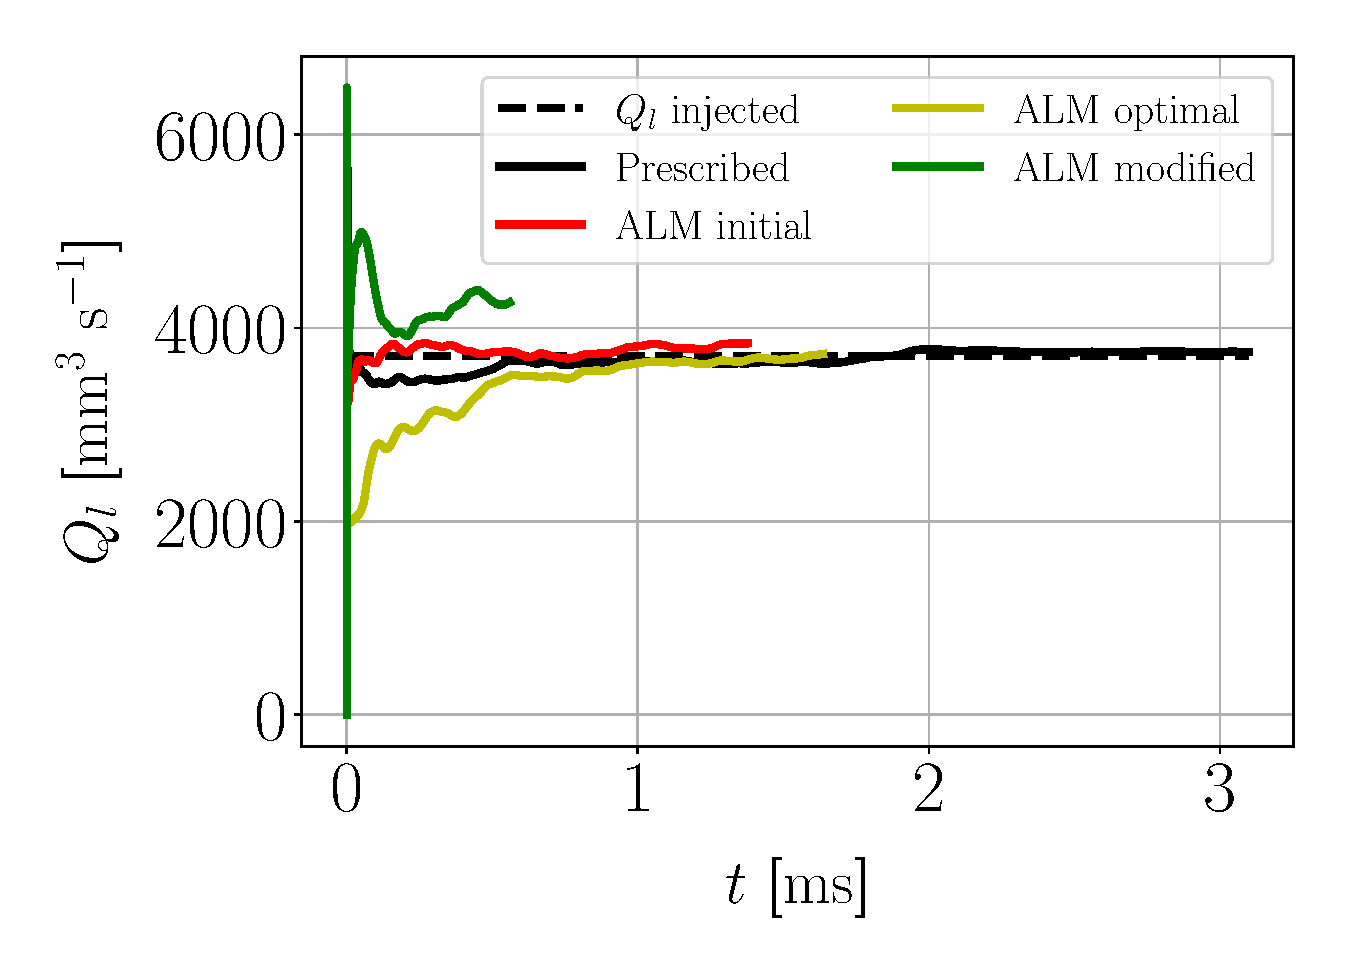
\includegraphics[scale=0.36]{./part2_developments/figures_ch6_lagrangian_JICF/params_gaseous_initial_conditions/convergence_Ql}
   %\caption{}
   %\label{} 
\end{subfigure}
\hspace{0.4in}
\begin{subfigure}[b]{0.45\textwidth}
	\centering
   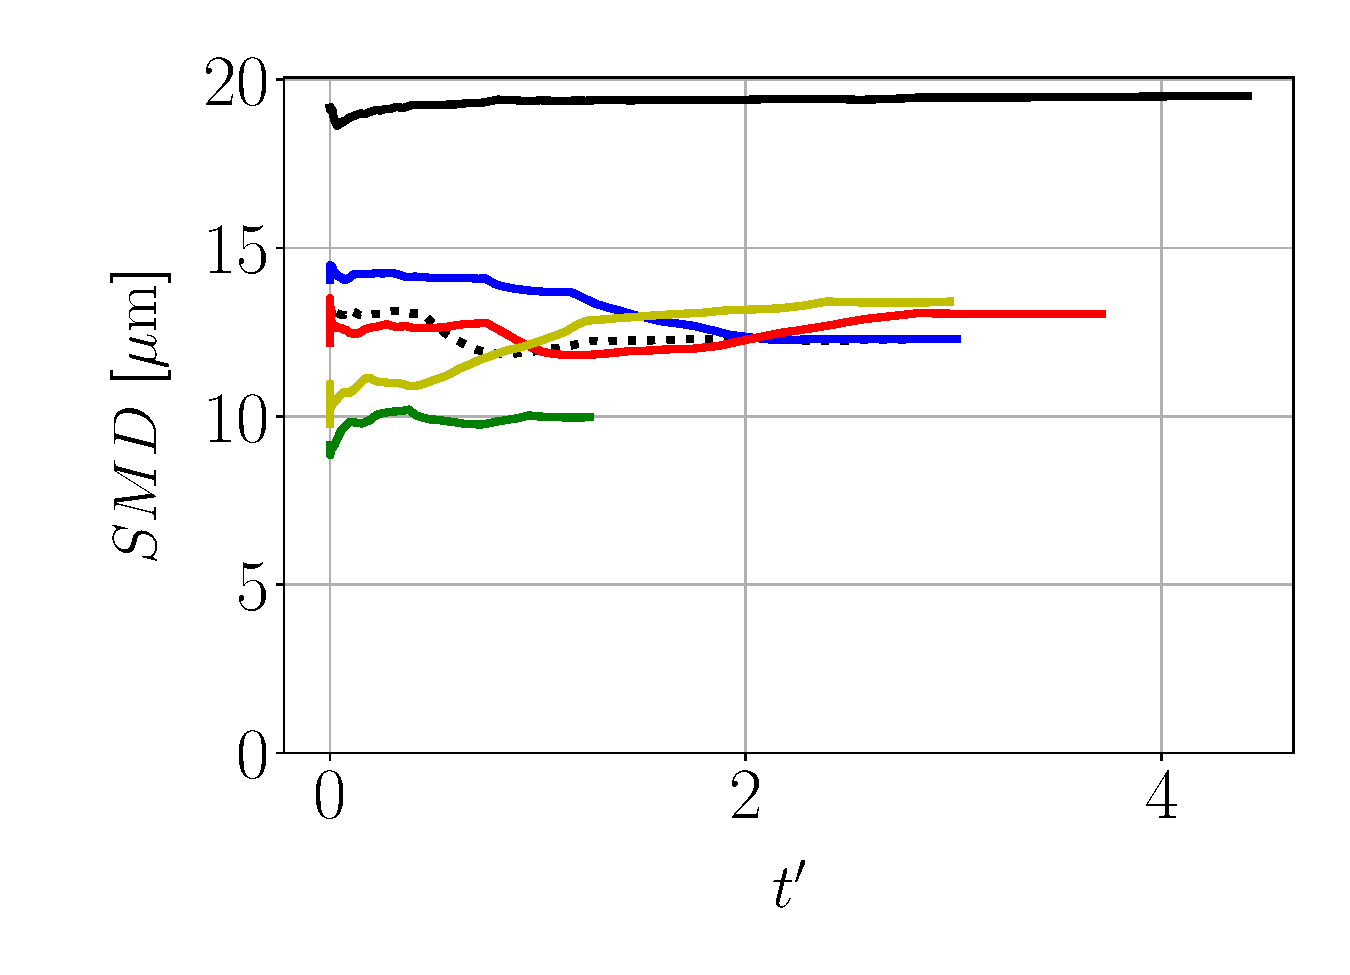
\includegraphics[scale=0.36]{./part2_developments/figures_ch6_lagrangian_JICF/params_gaseous_initial_conditions/convergence_SMD}
   %\caption{}
   %\label{}
\end{subfigure}
\caption{Convergence of spray liquid flux (\textsl{left}) and SMD (\textsl{right}) with time at plane $x = 80$ mm}
\label{fig:LGS_QL_and_SMD_convergence_with_time}
\end{figure}



\subsubsection*{Spatial evolution of spray}

\begin{figure}[h!]
\centering
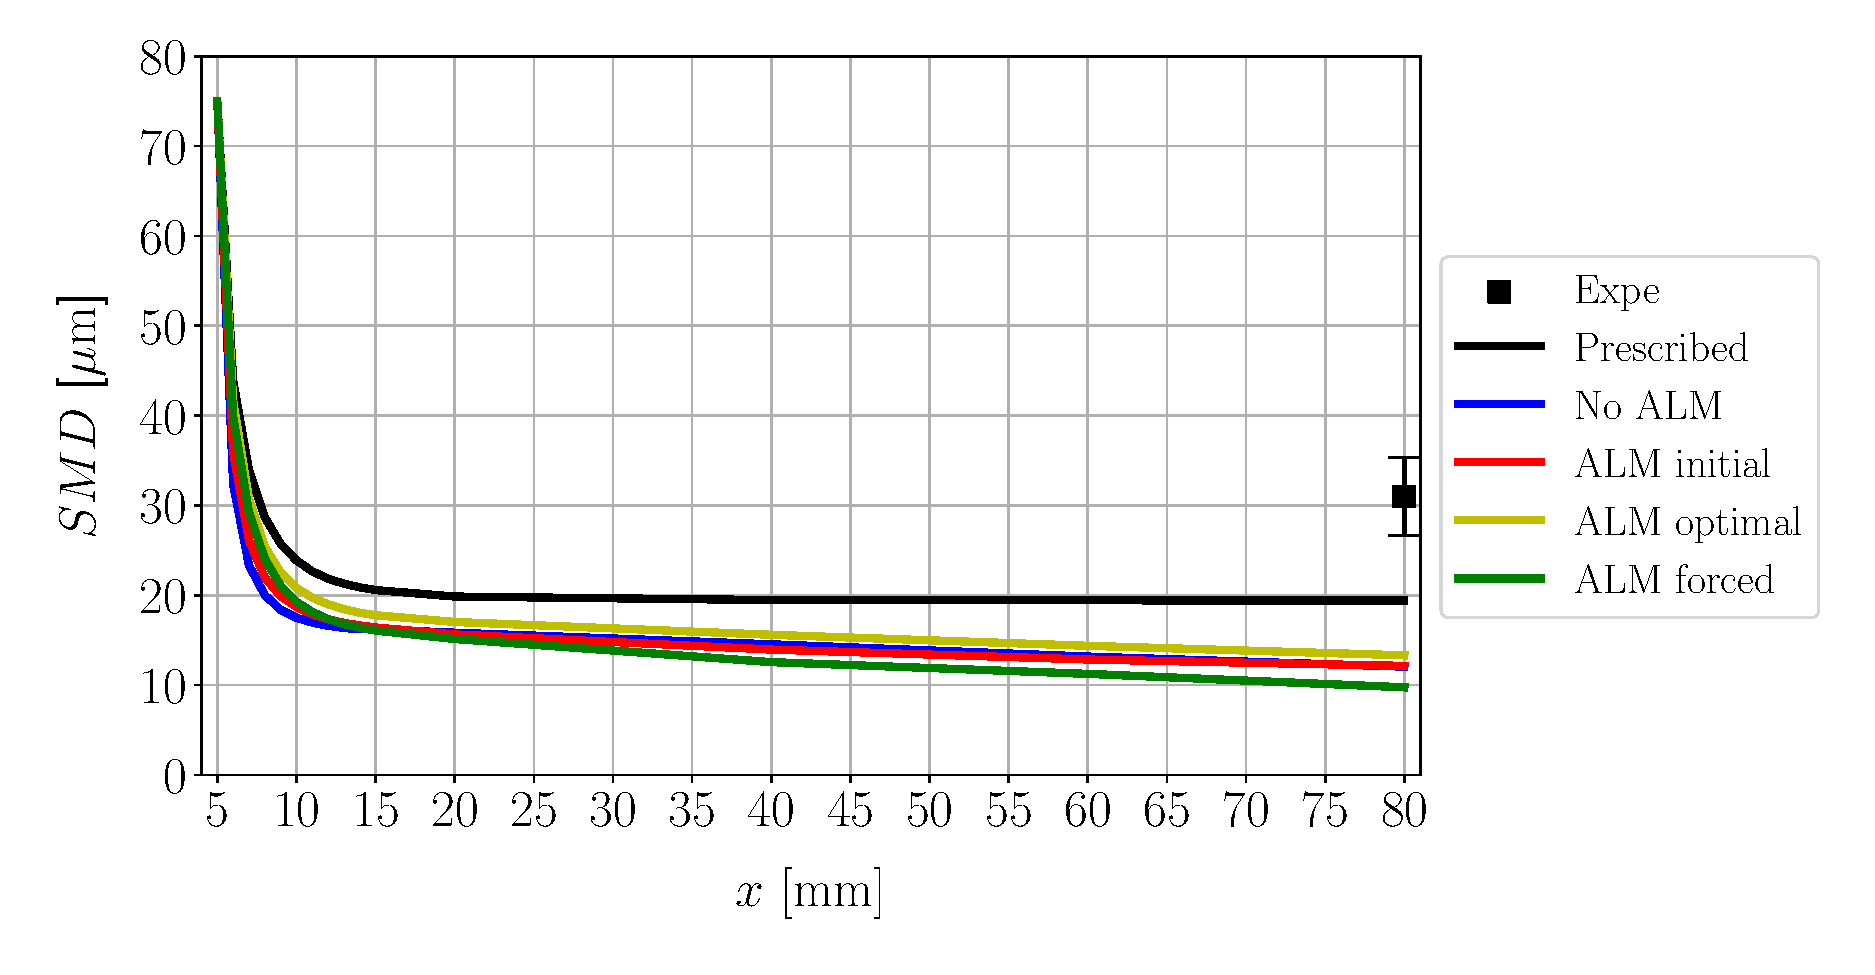
\includegraphics[scale=0.45]{./part2_developments/figures_ch6_lagrangian_JICF/params_gaseous_initial_conditions/SMD_vs_x_gaseous_BCs_comparison}
\vspace*{-0.4in}
\caption[Evolution of SMD along axial location $x$ for the different gaseous boundary conditions tested]{Evolution of SMD along axial location $x$ for the different gaseous boundary conditions tested. The SMD at $x = 5$ and $10$ mm for the resolved atomization case UG100\_DX10 is also added for comparison}
\label{fig:SMD_vs_x_param_gaseous_BCs}
\end{figure}


Since there is a strong reduction of particles diameters due to secondary atomization, it is of interest to see at which extent atomization acts along the channel. For this purpose, the evolution of $SMD$ with axial distance $x$ along the plenum is plotted in Figure \ref{fig:SMD_vs_x_param_gaseous_BCs}. The $SMD$ from the resolved simulation UG100\_DX10 and the experimental one with its uncertainties are also shown for comparison. As observed, the $SMD$ drops drastically shortly after injection up to $x \sim 20$ mm, then it continues decreasing in a linear way up to $x = 80$ mm. The abrupt decrease in diameter at early axial locations is exponential and shows a similar shape for all cases;  however, for the ALM cases, the decaying rate and the final $SMD$ varies. In general, the prescribed inlet provides the largest $SMD$ while the ALM cases result in lower values due to a worse replication of the resolved gaseous phase, thus mispredicting the relative velocity for the lagrangian droplets and affecting breakup. At $x = 10$ mm the deviation with the resolved case is large: 79.9 vs 23.9 $\mu$m for the prescribed inlet, which supposes a difference of 70 $\%$.  However,  the resolved atomization simulation might not be fine enough to retrieve the smallest liquid scales that would be actually present (as discussed in $\S$\ref{subsec:ch5_sec_spray_characterization}), hence limiting the smallest droplets that can be resolved.


The linear region, which spans from $x = 20$ to $80$ mm, reduces the mean diameter slowly along the channel after the disminution in the exponenial region. This is specially noticeable for the cases with the full computational domain from the resolved simulation (with and without ALM), while in the prescribed gaseous inlet simulation the variation is so small that is not appreciated in the figure. For quantifying this variation, a decay rate $\lambda$ is calculated as the slope in the $SMD$-$x$ curve from $x =20$ mm to $x = 80$ mm:

\begin{equation}
\lambda = \frac{SMD_{x=20\mathrm{mm}} -  SMD_{x=80\mathrm{mm}}}{60}
\end{equation} 

Table \ref{tab:SMD_decay_rates} summarizes the obtained SMDs and decay rates for all cases. The values for $\lambda$ are of the same order for all ALM and the unperturbed cases, while it is more than one order of magnitude lower than for the prescribed gaseous inlet spray. The lower decay rate is associated to a more accurate resolution of the gaseous phase with the prescribed inlet (meaning that it matches better the perturbed field of the resolved atomization simulation), which can be seen for instance in the gaseous profiles of Figure \ref{fig:JICF_ICS_custom_lines_y0_along_x_ux_mean}. The decay rates for the ALM cases show similar orders of magnitude, yet the values also differ and affect the final SMDs obtained: the lowest value (which results in a higher final SMD) corresponds to the optimal case, while the highest decay rate has been obtained for the ALM forced. In general, the lower the decay rate (or in other words, the larger the final SMD), the better, since as observed in Figure \ref{fig:SMD_vs_x_param_gaseous_BCs} the SMDs found in the simulations underestimate the experimental results.


\begin{table}[!h]
\centering
\caption{SMD values at $x = 20, 80$ mm and decay rates $\lambda$ in the linear region}
\begin{tabular}{cccc}
\thickhline
Case & $SMD_{x=20\mathrm{mm}}~\left[\mu \mathrm{m} \right]$ & $SMD_{x=80\mathrm{mm}}~\left[\mu \mathrm{m} \right]$ & $\lambda~\left[\mu \mathrm{m} ~ \mathrm{mm}^{-1} \right]$ \\
\thickhline
Prescribed inlet & 20.23 & 19.52 & 8 $\cdot 10^{-3}$ \\
No perturbation & 16.42 & 12.30 & 128 $\cdot 10^{-3}$\\
ALM initial & 15.77 & 12.30 & 128 $\cdot 10^{-3}$ \\
ALM tilted & 17.20 & 13.05 & 116 $\cdot 10^{-3}$ \\
ALM optimal & 17.225 & 13.41 & 110 $\cdot 10^{-3}$ \\
ALM forced & 15.280 & 9.98 & 167 $\cdot 10^{-3}$ \\
\thickhline
\end{tabular}
\label{tab:SMD_decay_rates}
\end{table}






\subsubsection*{Experimental comparison}

The sprays at $x = 80$ mm can be compared with the experimental results reported at the same locations. In first place, the global SMDs shown graphically in Figure \ref{fig:SMD_vs_x_param_gaseous_BCs} are also summarized in Table \ref{tab:SMD_deviations_gaseous_inlet}, where where the error with respect to experiments $\varepsilon_{SMD}$ is calculated as:

\begin{equation}
\label{eq:error_expe_SMD_LGS_simus}
\varepsilon_{SMD} = \frac{SMD_\mathrm{simu} - SMD_\mathrm{expe}}{SMD_\mathrm{expe}}
\end{equation}

where $SMD_\mathrm{simu}$ and $SMD_\mathrm{expe}$ are the numerical and experimental SMDs at $x = 80$ mm respectively. Results show that (as already mentiones in the previous section) the gaseous prescribed inlet provides the better experimental match for global SMD, while the ALM forced case provides the largest deviation. %Among all actuator cases, the optimal ALM is the one giving the best experimental comparision, yet it is still worse than the prescribed inlet simulation. This demonstrates again the importance of properly retrieving the gaseous phase, since as seen graphically in Figure \ref{fig:SMD_vs_x_param_gaseous_BCs} it has a strong impact in lagrangian particles breakup. In particular, secondary atomization is of high relevance in the case studied since the injected droplets, obtained through resolved atomization simulations, are larger than the experimental SMDs reported further downstream by \citeColor[becker_breakup_2002]. The secondary atomization is then strongly affected by the gaseous boundary conditions, since capturing accurately the velocity fields would allow to better approximating the relative velocities, which are one of the governing parameters of the secondary atomization models since they are related to the Weber number (criterion to decide if atomization occurs or not) by a power of 2.



\begin{table}[!h]
\centering
\caption{SMD values at $x = 80$ mm and deviation with the experimental value for different gaseous conditions}
\begin{tabular}{ccc}
\thickhline
Case & $SMD~\left[\mu \mathrm{m} \right]$ & $\varepsilon_{SMD}~\left[\% \right]$ \\
\thickhline
Experiments & 31 & - \\
Prescribed inlet & 19.52 & -37.03 \\
No perturbation & 12.30 & -60.31 \\
ALM initial & 12.30 & -60.31 \\
ALM tilted & 13.05 & -57.90 \\
ALM optimal & 13.41 & -56.75 \\
ALM forced & 9.98 & -67.82 \\
\thickhline
\end{tabular}
\label{tab:SMD_deviations_gaseous_inlet}
\end{table}

The spray at $x = 80$ mm is then discretized to yield the spatial maps of SMD and flux in Figure \ref{fig:maps_LGS_JICF_gaseous_influence}. These spatial magnitudes can also be integrated in each direction with Eqs. (\ref{eq:integrated_results_Becker_expe_results}) to yield the spatially integrated profiles of Figure \ref{fig:profiles_LGS_JICF_gaseous_influence}. The experimental maps and profiles are also displayed for comparison. 

Flux maps show an elliptical pattern elongated along the vertical direction, while experiments show a circular shape. Simulations show a larger concentration of droplets in the center, which is reflected in higher local maximum fluxes whose vertical location agrees fairly well with the experiments. The prescribed gaseous inlet simulation captures accurately this location, while the ALM ones underestimate it slightly, as it is also reflected in the vertical profiles of Figure \ref{fig:profiles_LGS_JICF_gaseous_influence}.  The numerical spray vertical boundaries, observed both in the maps and in the vertical flux profiles of Figure \ref{fig:profiles_LGS_JICF_gaseous_influence}, show that these penetrate further than the experiments. Nevertheless, the overestimated upper boundary corresponds to areas with large SMD and low liquid fluxes ($q_l < 0.5~\mathrm{cm}^3/\mathrm{cm}^2\mathrm{s}$), corresponding then to a few large droplets with a more ballistic behaviour (due to a larger Stokes number) that travel further away in the vertical direction. Indeed, the boundaries for the regions with larger fluxes ($q_l > 0.5~\mathrm{cm}^3/\mathrm{cm}^2\mathrm{s}$) match their experimental equivalent ones. Similarly, lateral boundaries show droplets up to the channel walls, although these regions (generally for $|y| > 6$ mm) contain low fluxes. The vertical boundaries where $q_l > 0.5~\mathrm{cm}^3/\mathrm{cm}^2\mathrm{s}$ are located closer to the central plane than in the experiments, yielding the elliptical pattern in the computations. This might be caused by an underestimation of the lateral trajectory in the resolved atomization simulation, although this characteristic of the JICF has not been addressed in this work and a definitive statement cannot be performed. The flux profiles integrated along the lateral  direction $\left\langle q_l \right\rangle \left( y \right)$ shows good experimental agreement for $y < 0$ but underestimation of flux for $y > 0$, which might indicate that experiments overestimate the flux at this region. In general, it can be said that the dispersed-phase computations retrieve quantitatively the patterns of the flux with similar vertical boundaries, yet there are a small quantity of large droplets penetrating further away than in the experiments. Simulations also show vertical locations of the maximum fuel flux close to experiments: the prescribed case can accurately retrieve this location, while the ALM ones generally underestimate it.


The numerical SMD maps show layered profiles with droplets sizes increasing from the bottom to the top, which is the characteristic ballistic behaviour of JICF sprays. This ballistic profile is also confirmed by the increasing SMD along $z$ in the profiles from Figure \ref{fig:profiles_LGS_JICF_gaseous_influence}. As shown both in the maps and profiles, all cases underestimate the experimental values (which agrees with the previous discussions on the global granulometry of the sprays). Most maps also reveal an increase in SMD towards the lateral edges, which is also reflected at the integrated profile $\left\langle SMD \right\rangle \left( y \right)$ in Figure \ref{fig:profiles_LGS_JICF_gaseous_influence} right (convex profile). Such behaviour, which is not observed in experiments but was also retrieved numerically by \citeColor[rachner_modelling_2002] (Figure \ref{fig:previous_works_profiles_comparison_with_expe}), is caused by large droplets following their own direction rather than being entrained by the flow, which reach the walls of the plenum and do not undergo further atomization. This lateral increase is clearly noticeable for the prescribed inlet simulation and less pronounced for the ALM ones: as secondary atomization acts faster for the latter, the larger droplets are quickly disintegrated and smaller droplets are obtained. Actually, the lateral profiles become flatter as the cases underestimate the SMDs, producing even a concave profile in the ALM forced simulation.





\clearpage

%\subsection{Vertical trajectories of lagrangian sprays}

\begin{figure}[h!]
\flushleft
\begin{subfigure}[b]{0.2\textwidth}
	\flushleft
%	\hspace*{-0.35in}
   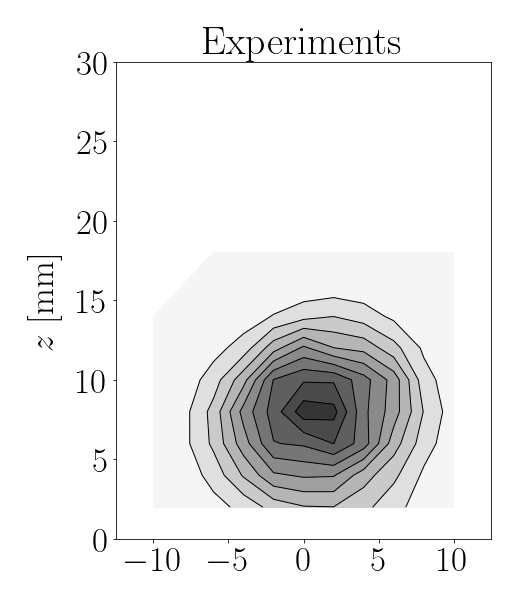
\includegraphics[scale=0.4]{./part2_developments/figures_ch6_lagrangian_JICF/params_gaseous_initial_conditions/maps/expe_flux}
   %\label{} 
\end{subfigure}
\hspace*{0.275in}
\begin{subfigure}[b]{0.2\textwidth}
	\flushleft
   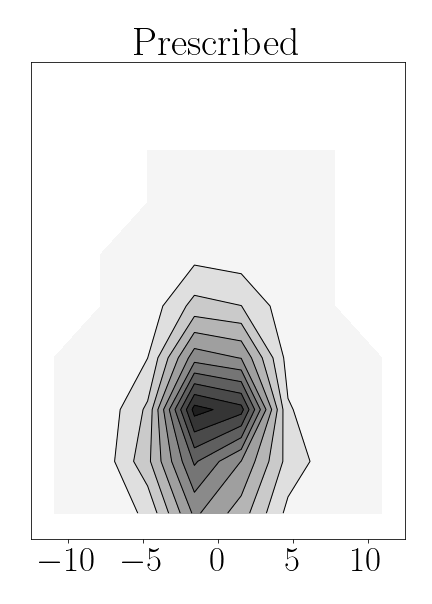
\includegraphics[scale=0.4]{./part2_developments/figures_ch6_lagrangian_JICF/params_gaseous_initial_conditions/maps/prescribed_flux}
   %\label{} 
\end{subfigure}
\hspace*{0.00in}
\begin{subfigure}[b]{0.2\textwidth}
	\flushleft
   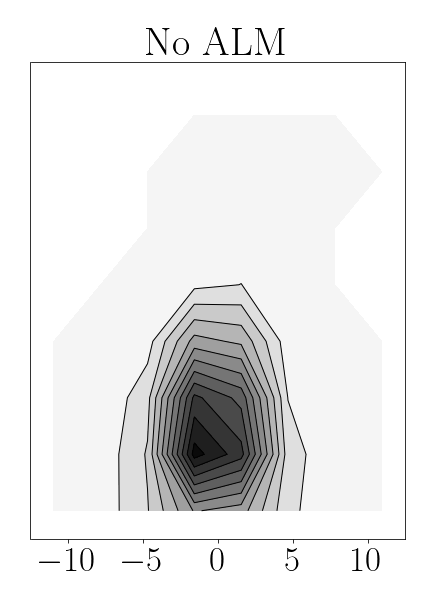
\includegraphics[scale=0.4]{./part2_developments/figures_ch6_lagrangian_JICF/params_gaseous_initial_conditions/maps/no_ALM_flux}
   %\label{} 
\end{subfigure}
\hspace*{0.00in}
\begin{subfigure}[b]{0.2\textwidth}
	\flushleft
   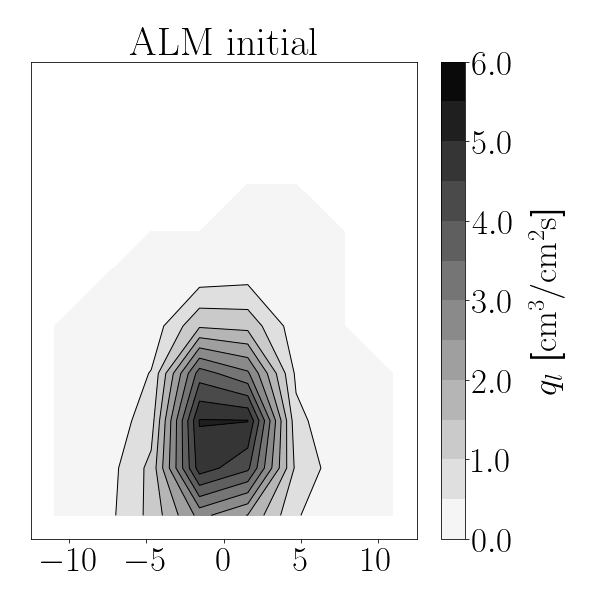
\includegraphics[scale=0.4]{./part2_developments/figures_ch6_lagrangian_JICF/params_gaseous_initial_conditions/maps/ALM_initial_flux}
   %\label{} 
\end{subfigure}

\vspace*{-0.25in}

\flushleft
\begin{subfigure}[b]{0.2\textwidth}
	\flushleft
%	\hspace*{-0.35in}
   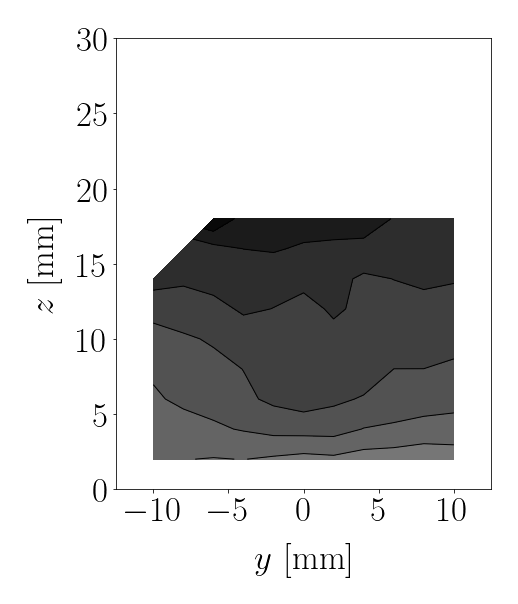
\includegraphics[scale=0.4]{./part2_developments/figures_ch6_lagrangian_JICF/params_gaseous_initial_conditions/maps/expe_SMD}
   %\label{} 
\end{subfigure}
\hspace*{0.25in}
\begin{subfigure}[b]{0.2\textwidth}
	\flushleft
   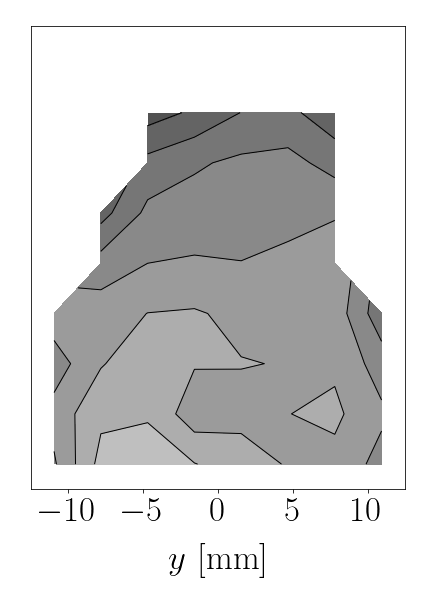
\includegraphics[scale=0.4]{./part2_developments/figures_ch6_lagrangian_JICF/params_gaseous_initial_conditions/maps/prescribed_SMD}
   %\label{} 
\end{subfigure}
\hspace*{0.00in}
\begin{subfigure}[b]{0.2\textwidth}
	\flushleft
   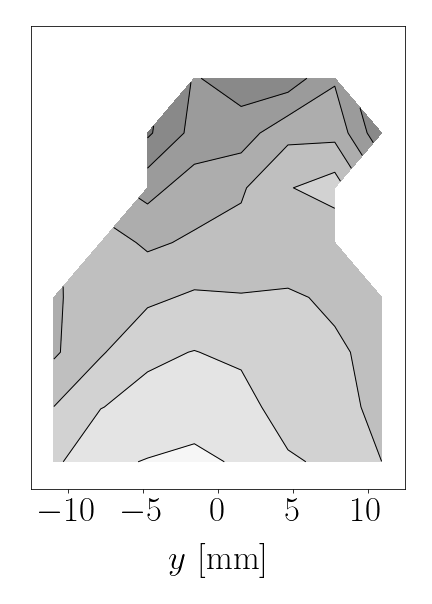
\includegraphics[scale=0.4]{./part2_developments/figures_ch6_lagrangian_JICF/params_gaseous_initial_conditions/maps/no_ALM_SMD}
   %\label{} 
\end{subfigure}
\hspace*{0.00in}
\begin{subfigure}[b]{0.2\textwidth}
	\flushleft
   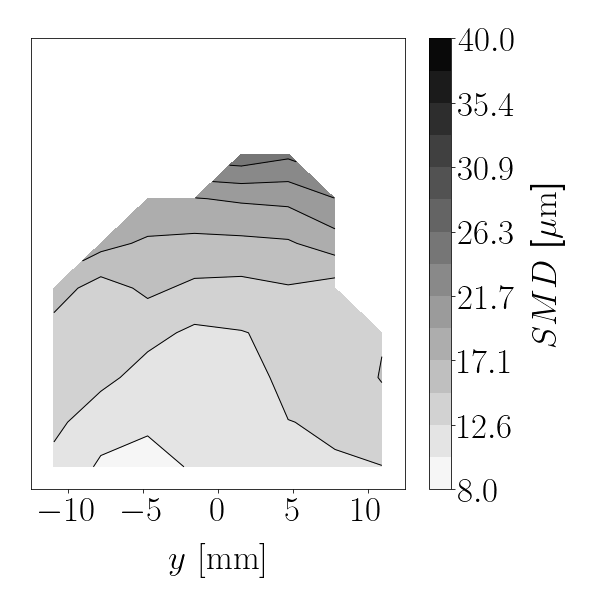
\includegraphics[scale=0.4]{./part2_developments/figures_ch6_lagrangian_JICF/params_gaseous_initial_conditions/maps/ALM_initial_SMD}
   %\label{} 
\end{subfigure}

\vskip\baselineskip

\begin{subfigure}[b]{0.2\textwidth}
	\flushleft
%	\hspace*{-0.35in}
   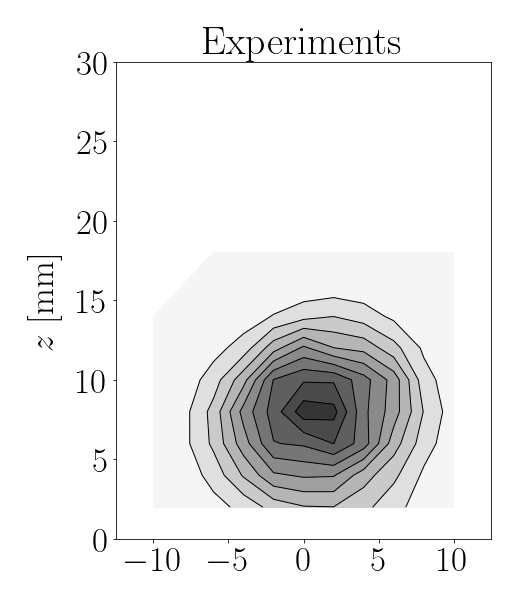
\includegraphics[scale=0.4]{./part2_developments/figures_ch6_lagrangian_JICF/params_gaseous_initial_conditions/maps/expe_flux}
   %\label{} 
\end{subfigure}
\hspace*{0.25in}
\begin{subfigure}[b]{0.2\textwidth}
	\flushleft
   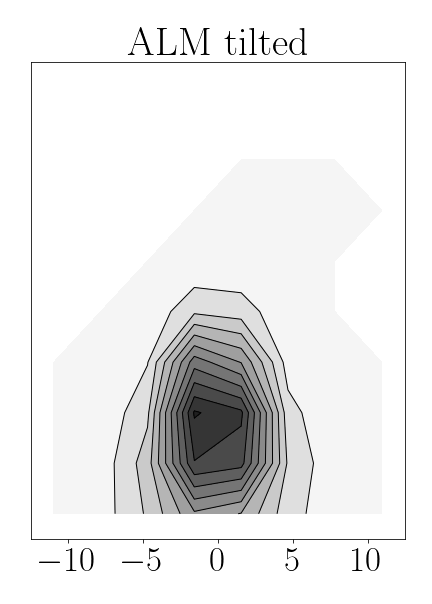
\includegraphics[scale=0.4]{./part2_developments/figures_ch6_lagrangian_JICF/params_gaseous_initial_conditions/maps/ALM_FDC_0p10_flux}
   %\label{} 
\end{subfigure}
\hspace*{0.00in}
\begin{subfigure}[b]{0.2\textwidth}
	\flushleft
   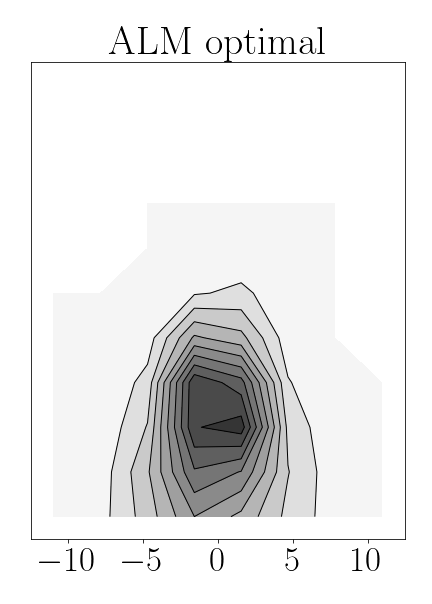
\includegraphics[scale=0.4]{./part2_developments/figures_ch6_lagrangian_JICF/params_gaseous_initial_conditions/maps/ALM_FDC_0p24_flux}
   %\label{} 
\end{subfigure}
\hspace*{0.00in}
\begin{subfigure}[b]{0.2\textwidth}
	\flushleft
   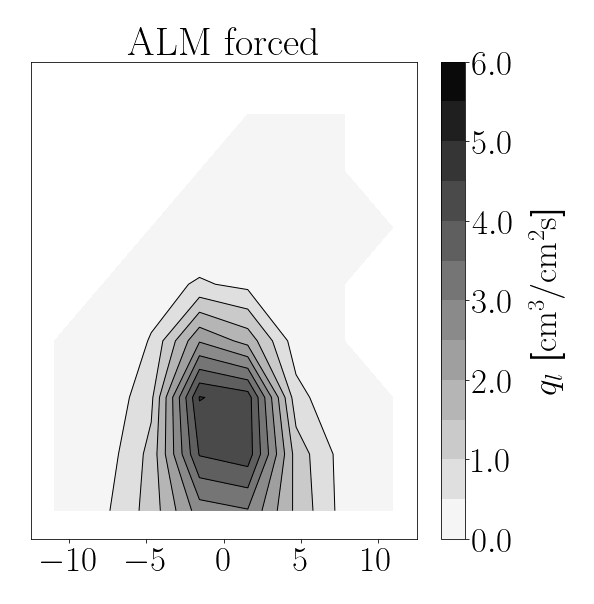
\includegraphics[scale=0.4]{./part2_developments/figures_ch6_lagrangian_JICF/params_gaseous_initial_conditions/maps/ALM_FDC_0p30_flux}
   %\label{} 
\end{subfigure}

\vspace*{-0.25in}

\flushleft
\begin{subfigure}[b]{0.2\textwidth}
	\flushleft
%	\hspace*{-0.35in}
   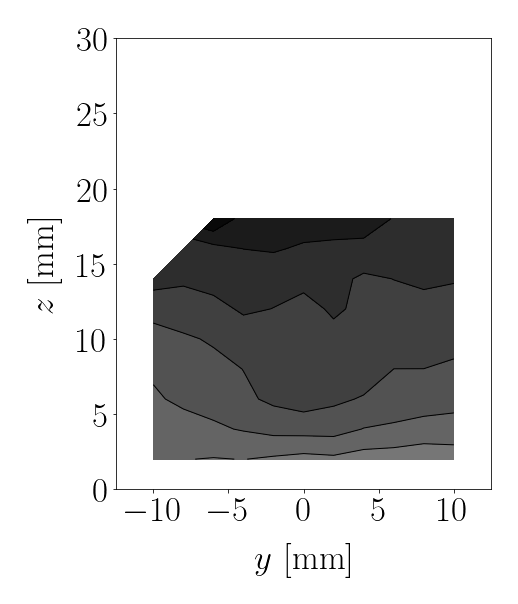
\includegraphics[scale=0.4]{./part2_developments/figures_ch6_lagrangian_JICF/params_gaseous_initial_conditions/maps/expe_SMD}
   %\label{} 
\end{subfigure}
\hspace*{0.25in}
\begin{subfigure}[b]{0.2\textwidth}
	\flushleft
   \includegraphics[scale=0.4]{./part2_developments/figures_ch6_lagrangian_JICF/params_gaseous_initial_conditions/maps/ALM_FDC_0p10_SMD}
   %\label{} 
\end{subfigure}
\hspace*{0.00in}
\begin{subfigure}[b]{0.2\textwidth}
	\flushleft
   \includegraphics[scale=0.4]{./part2_developments/figures_ch6_lagrangian_JICF/params_gaseous_initial_conditions/maps/ALM_FDC_0p24_SMD}
   %\label{} 
\end{subfigure}
\hspace*{0.00in}
\begin{subfigure}[b]{0.2\textwidth}
	\flushleft
   \includegraphics[scale=0.4]{./part2_developments/figures_ch6_lagrangian_JICF/params_gaseous_initial_conditions/maps/ALM_FDC_0p30_SMD}
   %\label{} 
\end{subfigure}

\caption{Flux and SMD maps for numerical simulations comparing the effect of gaseous phase modelling with the experimental results}
\label{fig:maps_LGS_JICF_gaseous_influence}
\end{figure}














\clearpage



\begin{figure}[h!]
\flushleft
\begin{subfigure}[b]{0.2\textwidth}
	\flushleft
   \includegraphics[scale=0.35]{./part2_developments/figures_ch6_lagrangian_JICF/params_gaseous_initial_conditions/profiles/flux_along_z}
   %\label{} 
\end{subfigure}
\hspace*{0.5in}
\begin{subfigure}[b]{0.2\textwidth}
	\flushleft
   \includegraphics[scale=0.35]{./part2_developments/figures_ch6_lagrangian_JICF/params_gaseous_initial_conditions/profiles/SMD_along_z}
   %\label{} 
\end{subfigure}
\hspace*{0.1in}
\begin{subfigure}[b]{0.4\textwidth}
	\flushleft
   \includegraphics[scale=0.35]{./part2_developments/figures_ch6_lagrangian_JICF/params_gaseous_initial_conditions/profiles/flux_along_y}\\
   \vspace{-0.16in}
   \includegraphics[scale=0.35]{./part2_developments/figures_ch6_lagrangian_JICF/params_gaseous_initial_conditions/profiles/SMD_along_y}
   %\label{} 
\end{subfigure}

\caption{Integrated profiles of flux and SMD maps for numerical simulations comparing the effect of gaseous phase modelling with the experimental results}
\label{fig:profiles_LGS_JICF_gaseous_influence}
\end{figure}

The analysis from this section has shown that the imposition of accurate boundary conditions for the gaseous phase is paramount for a proper modelling of JICF dispersed-phase simulations, as the gaseous flow field will affect the secondary atomization of the droplets through the liquid-gas relative velocity. The prescribed gaseous inlet methodology has found to retrieve more accurately the experimental results, and therefore it will be kept for the subsequent studies in this chapter.





\section{Influence of secondary atomization model}
\label{sec:SLI_LGS_secondary_breakup_models}

To consider the secondary breakup of lagrangian droplets in dispersed-phase simulations, three atomization models are available ($\S$\ref{sec:ch4_secondary_atomization_modeling}): TAB, ETAB and Gorokhovski. All these models estimate breakup according to the Weber based on the relative velocity, which is the known parameter to control secondary atomization. Then, the exact instant of breakup and the size and number of children droplets are calculated differently by each model. The TAB and ETAB models belong to the same family and provide fixed values for the parameters controlling the model, while the Gorokhovski's stochastic model presents two constants ($K_1$, $K_2$) that can be chosen by the user. These constants were calibrated to better match the experimental results: the values  $K_1 = 0.05$, $K_2 = 1.0$ were retrieved since they yield the lowest error in SMD with respect to experiments (results from the calibration analysis are provided in Appendix \ref{app:second_atom_goro_calibration}). In this section, all the three models are compared in three different dispersed-phase simulations. \\

The SMD maps are displayed in Figure \ref{fig:maps_LGS_JICF_second_atom_models}, and their corresponding integrated profiles in Figure \ref{fig:profiles_LGS_JICF_secondary_atom_model}. Both TAB and ETAB models produce similar circular patterns for the fluxes. Spray from TAB model overpredicts the vertical maximum flux location, also condensing a large part of the spray in this region as shown by the larger local fluxes. The ETAB model, on the other hand, predicts this location accurately and shows a good spatial repartition of the spray. This model also retrieves properly the experimental vertical bounds as reflected both in the map and the integrated profile $\left\langle q_l \right\rangle \left( z \right)$. The SMD maps and profiles show a proper ballistic behaviour for both TAB and ETAB sprays but an underestimation of the diameters, those being specially small for the TAB model. Underprediction of particles sizes by the TAB model is a known downcome of this model \citepColor[tanner_liquid_1997], and solving this issue was the reason why the ETAB model was developed. Indeed, the figures show that the latter model produces larger droplets than the former: the SMDs at $x = 80$ mm, summarized in Table \ref{tab:SMD_deviations_breakup_model}, yield errors of $- 55.07~\%$ and $43.59~\%$ for the TAB and ETAB models respectively. The closest is then obtained for the Gorokhovski model.

\clearpage


\begin{figure}[t!]
\flushleft
\begin{subfigure}[b]{0.2\textwidth}
	\flushleft
%	\hspace*{-0.35in}
   \includegraphics[scale=0.4]{./part2_developments/figures_ch6_lagrangian_JICF/params_breakup_model/maps/expe_flux}
   %\label{} 
\end{subfigure}
\hspace*{0.27in}
\begin{subfigure}[b]{0.2\textwidth}
	\flushleft
   \includegraphics[scale=0.4]{./part2_developments/figures_ch6_lagrangian_JICF/params_breakup_model/maps/goro_flux}
   %\label{} 
\end{subfigure}
\hspace*{0.02in}
\begin{subfigure}[b]{0.2\textwidth}
	\flushleft
   \includegraphics[scale=0.4]{./part2_developments/figures_ch6_lagrangian_JICF/params_breakup_model/maps/TAB_flux}
   %\label{} 
\end{subfigure}
\hspace*{0.02in}
\begin{subfigure}[b]{0.2\textwidth}
	\flushleft
   \includegraphics[scale=0.4]{./part2_developments/figures_ch6_lagrangian_JICF/params_breakup_model/maps/ETAB_flux}
   %\label{} 
\end{subfigure}

\vspace*{-0.25in}

\flushleft
\begin{subfigure}[b]{0.2\textwidth}
	\flushleft
%	\hspace*{-0.35in}
   \includegraphics[scale=0.4]{./part2_developments/figures_ch6_lagrangian_JICF/params_breakup_model/maps/expe_SMD}
   %\label{} 
\end{subfigure}
\hspace*{0.27in}
\begin{subfigure}[b]{0.2\textwidth}
	\flushleft
   \includegraphics[scale=0.4]{./part2_developments/figures_ch6_lagrangian_JICF/params_breakup_model/maps/goro_SMD}
   %\label{} 
\end{subfigure}
\hspace*{0.02in}
\begin{subfigure}[b]{0.2\textwidth}
	\flushleft
   \includegraphics[scale=0.4]{./part2_developments/figures_ch6_lagrangian_JICF/params_breakup_model/maps/TAB_SMD}
   %\label{} 
\end{subfigure}
\hspace*{0.02in}
\begin{subfigure}[b]{0.2\textwidth}
	\flushleft
   \includegraphics[scale=0.4]{./part2_developments/figures_ch6_lagrangian_JICF/params_breakup_model/maps/ETAB_SMD}
   %\label{} 
\end{subfigure}



\caption{Flux and SMD maps for numerical simulations comparing the effect of secondary atomization models with the experimental results}
\label{fig:maps_LGS_JICF_second_atom_models}
\end{figure}


\begin{figure}[h!]
\flushleft
\begin{subfigure}[b]{0.2\textwidth}
	\flushleft
   \includegraphics[scale=0.35]{./part2_developments/figures_ch6_lagrangian_JICF/params_breakup_model/profiles/flux_along_z}
   %\label{} 
\end{subfigure}
\hspace*{0.5in}
\begin{subfigure}[b]{0.2\textwidth}
	\flushleft
   \includegraphics[scale=0.35]{./part2_developments/figures_ch6_lagrangian_JICF/params_breakup_model/profiles/SMD_along_z}
   %\label{} 
\end{subfigure}
\hspace*{0.1in}
\begin{subfigure}[b]{0.4\textwidth}
	\flushleft
   \includegraphics[scale=0.35]{./part2_developments/figures_ch6_lagrangian_JICF/params_breakup_model/profiles/flux_along_y}\\
   \vspace{-0.16in}
   \includegraphics[scale=0.35]{./part2_developments/figures_ch6_lagrangian_JICF/params_breakup_model/profiles/SMD_along_y}
   %\label{} 
\end{subfigure}

\caption{Integrated profiles of flux and SMD maps for numerical simulations comparing the effect of secondary atomization models with the experimental results}
\label{fig:profiles_LGS_JICF_secondary_atom_model}
\end{figure}




\clearpage

\begin{table}[!h]
\centering
\caption{SMD values at $x = 80$ mm for simulations with the different secondary atomization models}
\begin{tabular}{ccc}
\thickhline
Case & $SMD~\left[\mu \mathrm{m} \right]$ & $\varepsilon_{SMD}~\left[\% \right]$ \\
\thickhline
Experiments & 31 & - \\
Gorokhovski & 19.44 & -37.29 \\
TAB & 13.93 & -55.07 \\
ETAB & 17.49 & -43.59 \\
\thickhline
\end{tabular}
\label{tab:SMD_deviations_breakup_model}
\end{table}

Evolution of the SMD along the channel is plotted in Figure \ref{fig:SMD_vs_x_param_breakup_model}. The SMD shows also a sharp reduction close to injection, with a faster decay for the TAB than for the ETAB and Gorokhovski models. The models from the TAB family stabilize at $x \sim 15$ mm, earlier than Gorokhovski. From this graph, it is demonstrated that the earliest instants are crucial for the atomization process, since the lowests SMDs are always obtained for the largest decay rates close to injection. Such abrupt decay rates very close to injection occur due to large relative velocities, as momentum exchange between the liquid and the gas has not occured yet. Momentum exchange is assessed later in $\S$\ref{sec:LGS_delay_secon_atom} by introducing an artificial delay from injection to the onset of atomization.


\begin{figure}[h!]
\centering
\includegraphics[scale=0.475]{./part2_developments/figures_ch6_lagrangian_JICF/params_breakup_model/SMD_vs_x_breakup_models_comparison}
\vspace*{-0.4in}
\caption[Evolution of SMD along axial location $x$ for the three atomization models]{Evolution of SMD along axial location $x$ for the three atomization models. The SMD at $x = 5$ and $10$ mm for the resolved atomization case UG100\_DX10 is also added for comparison}
\label{fig:SMD_vs_x_param_breakup_model}
\end{figure}

In general, it has been observed that the secondary atomization model has a great influence on the resulting lagrangian spray. The Gorokhovski model shows the best agreement in terms of spray sizes. Even so, all models tested do not yield particles sizes within the experimental range.  Nevertheless, these atomization models are general and have not been developed for particular conditions: the high pressure, highly turbulent environment found in the studied case might require atomization models more fitted to these conditions (indeed, both \citeColor[rachner_modelling_2002] and \citeColor[eckel_semi-empirical_2016] employed an ad-hoc atomization model particular for this operating condition). Furthermore, this work has not considered the coalescence of lagrangian droplets, which in reality could produce larger diameters after the atomization process.









\clearpage

\section{Influence of spray injection variables}
\label{sec:effect_of_SLI_variables}

In this section, the sensitivity of the dispersed-phase simulations to the parameters that can be prescribed with SLI is assessed. These parameters are summarized in the corresponding block of Figure \ref{fig:dispersed_phase_sli_parameters}. For performing these simulations, the prescribed gaseous inlet is chosen as boundary condition for the gas phase, and the Gorokhovski model is applied, as justified by the analyses performed in the last sections.


\subsection{Level-set resolution and injection location}
\label{subsec:SLI_LGS_resolution_and_injection_location}


Firstly, the influence of the injection location and the level-set resolution are assessed. For the former one, the SLIs obtained at $x = 10$ mm shown in Figure \ref{fig:injectors_sli_uG100_dx10_x10} are injected in the prescribed inlet which replicates the gaseous field for case UG100\_DX10. For the latter, the SLIs at $x = 5$ and 10 mm  from case UG100\_DX20 (respectively Figures \ref{fig:injectors_sli_uG100_dx20_x05} and \ref{fig:injectors_sli_uG100_dx20_x10}) are plugged into an aerodynamic field obtained by prescribing the gaseous phase statistics from this resolved case. Each case is named as its corresponding resolved atomization simulation plus its injection location: for instance, the baseline case is named UG100\_DX10\_x05 since it uses the SLI from resolved simulation UG100\_DX10 at the location $x = 5$ mm.


\begin{figure}[h!]
\flushleft
\begin{subfigure}[b]{0.2\textwidth}
	\flushleft
   \includegraphics[scale=0.35]{./part2_developments/figures_ch6_lagrangian_JICF/params_resol_and_xInj/profiles/flux_along_z}
   %\label{} 
\end{subfigure}
\hspace*{0.5in}
\begin{subfigure}[b]{0.2\textwidth}
	\flushleft
   \includegraphics[scale=0.35]{./part2_developments/figures_ch6_lagrangian_JICF/params_resol_and_xInj/profiles/SMD_along_z}
   %\label{} 
\end{subfigure}
\hspace*{0.1in}
\begin{subfigure}[b]{0.4\textwidth}
	\flushleft
   \includegraphics[scale=0.35]{./part2_developments/figures_ch6_lagrangian_JICF/params_resol_and_xInj/profiles/flux_along_y}\\
   \vspace{-0.16in}
   \includegraphics[scale=0.35]{./part2_developments/figures_ch6_lagrangian_JICF/params_resol_and_xInj/profiles/SMD_along_y}
   %\label{} 
\end{subfigure}
\vspace*{-0.1in}
\caption{Integrated profiles of flux and SMD maps for numerical simulations comparing the effect of SLIs obtained with different resolutions and at several injection locations with the experimental results}
\label{fig:profiles_LGS_JICF_resol_and_xInj}
\end{figure}

Profiles for the integrated SMD and flux are shown in Figure \ref{fig:profiles_LGS_JICF_resol_and_xInj}. The effect of the level-set resolution on the dispersed-phase spray is clearly remarkable: vertical flux profiles shows their maximum flux location in the coarse cases (UG100\_DX20) at a position closer to the wall, which does not agree with the experiments (the fine simulations UG100\_DX10 capture it accurately). This is a consequence of the lower vertical penetration from the resolved jets with the coarse resolution (see trajectories in Figure \ref{fig:JICF_trajectories_validation}). The vertical boundaries for the coarse SLIs are similar to the fine ones, and even higher for case UG100\_DX20\_x10. This is attributed to big particles being injected in these computations: droplets with larger diameters will travel along the vertical direction for longer than the smaller ones from the fine simulations until they atomize and relax towards the crossflow direction. Yet, such droplets are located in very low flux regions and do not represent a large portion of the spray. 

Particles are generally larger for the coarse SLI simulations than for the fine one. The vertical SMD profiles show a more pronounced ballistic behaviour for case UG100\_DX20\_x05, caused by larger droplets sampled at the top part of the spray. These droplets, which can be seen in the snapshot of Figure \ref{fig:JICF_dx20_large_droplets}, are very large particles injected at $x = 5$ mm which are convected along the channel without undergoing atomization. They were found to be surrounded by a cluster of smaller particles that might affect the gaseous phase in ensemble, preventing them from atomizing. Furthermore, since these particles are introduced from the beginning of the simulation, the SMD evolution along the channel will also be affected. This is shown in Figure \ref{fig:SMD_vs_x_param_LS_resol_and_xinj}: simulation UG100\_DX20\_x05 captures a SMD decay with different rates compared to the rest of the cases. On the other hand, computation UG100\_DX20\_x10 does not show over-estimated ballistic profiles, and its SMD evolution along the channel shows a profile such as the ones previously observed: a clear exponential decay right after injection followed by a linear decrease afterwards. This demonstrates that for the coarse case it is better to inject downstream, since the spray from the resolved simulation is better atomized. In terms of global size, the SMDs at $x = 80$ mm summarized in Table \ref{tab:SMD_deviations_turb_inj} show that the coarser simulations produce larger droplets, which approach the experimental results. Nevertheless, this is a consequence of larger droplets being injected, which atomize through a breakup cascade into smaller and smaller particles, and end up reaching equilibrium with the ambient gas at larger diameters than in the fine simulations. The results for the vertical flux profiles from Figure \ref{fig:profiles_LGS_JICF_resol_and_xInj} shows that, indeed, the coarse simulations do not capture accurately the vertical location of maximum flux, and hence it is better to initiate lagrangian computations with the finer injectors.

\begin{figure}[h!]
	\centering	\includeinkscape[inkscapelatex=false,scale=0.8]{./part2_developments/figures_ch6_lagrangian_JICF/params_resol_and_xInj/JICF_dx20_large_droplets}
	\caption{View of the dispersed spray in simulation UG100\_DX20\_x05, showing three regions with large droplets along the channel}
	\label{fig:JICF_dx20_large_droplets}
\end{figure}


%Larger droplets in the coarse simulations are consequence of the secondary atomization models, as it calculates the size of the children droplets in relation to the parent's diameter (Equation (\ref{eq:r_ch_goro})). These droplets are disintegrated into smaller ones through the cascade behaviour at the same time that they exchange momentum with the gaseous crossflow, reducing their relative velocity until they reach equilibrium with the gas. This equilibrium is reached then at larger diameters than in the fine SLI simulations, \hl{as shown by the spatial evolution of SMD at Figure XX}.

\vspace*{-0.2in}

\begin{figure}[h!]
\centering
\includegraphics[scale=0.5]{./part2_developments/figures_ch6_lagrangian_JICF/params_resol_and_xInj/SMD_vs_x_LS_resol_and_x_inj}
\vspace*{-0.4in}
\caption[Evolution of SMD along axial location $x$ with SLIs from two level-set resolutions UG100\_DX10, UG100\_DX20 at two injection locations]{Evolution of SMD along axial location $x$ with SLIs from two level-set resolution at two injection locations $x = 5, 10$ mm. The SMD at $x = 5$ and $10$ mm for the resolved atomizations are also added for comparison}
\label{fig:SMD_vs_x_param_LS_resol_and_xinj}
\end{figure}

With respect to injection location, the differences for the SLIs for the coarse simulations have already been discussed, showing greater differences in profiles and SMD evolution along the channel. Regarding the SLIs from the fine simulations, the corresponding dispersed-phase computations do not show relevant dependencies on the injection location: all integrated profiles are similar in shape and in values, and the global SMDs obtained are practically identical. This might suppose that injecting droplets through SLIs obtained from the fine resolutions at different locations would make no difference in the lagrangian spray at $x = 80$ mm. In such case, a resolved simulation could provide a SLI with cheaper computational costs than the ones reported in the previous chapter (Table \ref{fig:SLI_cost_convergence_all}), as the liquid removal sponge layer could be placed further upstream, for instance at $x = 6$ mm than at 11 mm, while retrieving an almost identical lagrangian spray in the dispersed-phase computation. This analysis reaffirms the idea that it is better to build a SLI with finer resolved atomization simulations: not only the particle's granulometry is better resolved than in an equivalent coarser simulation, but also a SLI can be built with a more reduced spatial domain due to a better atomization of the resolved droplets. It would be interesting to continue this study with even finer interface cell sizes in the resolved simulations, which has not been possible in this thesis due to the higher computational costs required. 


\begin{table}[!h]
\centering
\caption{SMD values at $x = 80$ mm for simulations with different SLIs}
\begin{tabular}{ccc}
\thickhline
Case & $SMD~\left[\mu \mathrm{m} \right]$ & $\varepsilon_{SMD}~\left[\% \right]$ \\
\thickhline
Experiments & 31 & - \\
UG100\_DX10\_x05 & 19.44 & -37.29 \\
UG100\_DX10\_x10 & 19.51 & -37.05 \\
UG100\_DX20\_x05 & 22.59 & -27.14 \\
UG100\_DX20\_x10 & 21.58 & -30.38 \\
\thickhline
\end{tabular}
\label{tab:SMD_deviations_turb_inj}
\end{table}



\subsection{Spray velocities}
\label{subsec:SLI_LGS_velocity_effects}

Prescribed velocities through SLI are investigated here by using different combinations of the parameters in Eq. (\ref{eq:ch4_lagrangian_injection_velocity_with_mean_and_rms}). For the previous cases, the mean velocity was volume weighted (VW) and the $r$ law was Gaussian, injecting then into each SLI probe a stochastic component representing the normal dispersion of the droplet's velocities. Here, the effect of mean velocity is seen by injecting the arithmetic mean velocity ($\overline{u}$) while keeping constant the $r$ law to follow a Gaussian distribution. Then, the effect of RMS is assessed by changing the $r$ law to a uniform distribution and by removing the RMS component of the velocity (zero law), these two modifications performed with volume-weighted mean velocity being injected. Figure \ref{fig:maps_SLI_with_arithmetic_mean_and_VW} shows the SLIs from simulation UG100\_DX10 at $x_\mathrm{inj} = 5$ mm with the arithmetic mean and VW velocities for visual comparison. Larger differences are found at the central and top parts of the maps, which are respectively the regions with larger flux and with larger droplets.% The maps for the axial and vertical velocities are the ones showing more differences: in general, the volume-weighted velocities are lower with respect to the arithmetic ones, which will affect secondary atomization since it modifies the relative liquid-gas velocity. For the vertical velocity map, this could also affect the penetration of the spray. The vertical velocity maps do not show significant differences, appart from a wider central region where velocity varies from $-6$ to $4$ m/s. 


\begin{figure}[ht]
\flushleft
\begin{subfigure}[b]{0.2\textwidth}
	\flushleft
	\hspace*{-0.45in}
   \includegraphics[scale=0.19]{./part2_developments/figures_ch6_lagrangian_JICF/injectors_SLI/uG100_dx10_x05_SMD_map}
   %\label{} 
\end{subfigure}
\hspace*{0.075in}
\begin{subfigure}[b]{0.2\textwidth}
	\flushleft
   \includegraphics[scale=0.19]{./part2_developments/figures_ch6_lagrangian_JICF/injectors_SLI/uG100_dx10_x05_ux_mean_map}
   %\label{} 
\end{subfigure}
\hspace*{0.45in}
\begin{subfigure}[b]{0.2\textwidth}
	\flushleft
   \includegraphics[scale=0.19]{./part2_developments/figures_ch6_lagrangian_JICF/injectors_SLI/uG100_dx10_x05_uy_mean_map}
   %\label{} 
\end{subfigure}
\hspace*{0.45in}
\begin{subfigure}[b]{0.2\textwidth}
	\flushleft
   \includegraphics[scale=0.19]{./part2_developments/figures_ch6_lagrangian_JICF/injectors_SLI/uG100_dx10_x05_uz_mean_map}
   %\label{} 
\end{subfigure}

\vspace*{-0.20in}

\flushleft
\begin{subfigure}[b]{0.2\textwidth}
	\flushleft
	\hspace*{-0.45in}
   \includegraphics[scale=0.19]{./part2_developments/figures_ch6_lagrangian_JICF/injectors_SLI/uG100_dx10_x05_volume_flux_map}
   %\label{} 
\end{subfigure}
\hspace*{0.075in}
\begin{subfigure}[b]{0.2\textwidth}
	\flushleft
   \includegraphics[scale=0.19]{./part2_developments/figures_ch6_lagrangian_JICF/injectors_SLI/uG100_dx10_x05_ux_mean_vw_map}
   %\label{} 
\end{subfigure}
\hspace*{0.45in}
\begin{subfigure}[b]{0.2\textwidth}
	\flushleft
   \includegraphics[scale=0.19]{./part2_developments/figures_ch6_lagrangian_JICF/injectors_SLI/uG100_dx10_x05_uy_mean_vw_map}
   %\label{} 
\end{subfigure}
\hspace*{0.45in}
\begin{subfigure}[b]{0.2\textwidth}
	\flushleft
   \includegraphics[scale=0.19]{./part2_developments/figures_ch6_lagrangian_JICF/injectors_SLI/uG100_dx10_x05_uz_mean_vw_map}
   %\label{} 
\end{subfigure}

\caption{SLI mean arithmetic and VW velocity maps from case UG100\_DX10 at $x_\mathrm{inj} = 5$ mm }
\label{fig:maps_SLI_with_arithmetic_mean_and_VW}
\end{figure}

\clearpage

Results are shown in Figure \ref{fig:profiles_LGS_JICF_spray_velocities}, where the integrated SMD and flux profiles are plotted. The largest differences are observed for the treatment of the average velocities, since the vertical profiles change drastically when either arithmetic mean or VW averages are considered. By prescribing the arithmetic mean, droplets penetrate further away than for VW. The reason is the larger vertical velocities injected with arithmetic means: as shown in Figure \ref{fig:maps_SLI_with_arithmetic_mean_and_VW}, droplets at the top of the spray are injected with faster vertical velocity, and since these droplets are larger, they travel further along the vertical direction. The imposition of a different liquid velocity field also affects secondary atomization, since as observed in the SMD vertical profile from Figure \ref{fig:profiles_LGS_JICF_spray_velocities} the droplets at the top part of the spray are smaller than at the bottom one, creating then a counter-ballistic behaviour which is not physical in such a JICF configuration. The flux profile also shows a flatter shape in the center of the spray instead of a peaky one, indicating concentration of droplets in a wide region around the spray center. Therefore, a proper prescription of accurate mean velocities is crucial for dispersed-phase simulations when using SLI. 


\begin{figure}[ht]
\flushleft
\begin{subfigure}[b]{0.2\textwidth}
	\flushleft
   \includegraphics[scale=0.35]{./part2_developments/figures_ch6_lagrangian_JICF/params_spray_velocities/profiles/flux_along_z}
   %\label{} 
\end{subfigure}
\hspace*{0.5in}
\begin{subfigure}[b]{0.2\textwidth}
	\flushleft
   \includegraphics[scale=0.35]{./part2_developments/figures_ch6_lagrangian_JICF/params_spray_velocities/profiles/SMD_along_z}
   %\label{} 
\end{subfigure}
\hspace*{0.1in}
\begin{subfigure}[b]{0.4\textwidth}
	\flushleft
   \includegraphics[scale=0.35]{./part2_developments/figures_ch6_lagrangian_JICF/params_spray_velocities/profiles/flux_along_y}\\
   \vspace{-0.16in}
   \includegraphics[scale=0.35]{./part2_developments/figures_ch6_lagrangian_JICF/params_spray_velocities/profiles/SMD_along_y}
   %\label{} 
\end{subfigure}

\caption{Integrated profiles of flux and SMD maps for numerical simulations comparing the effect of spray velocities with the experimental results}
\label{fig:profiles_LGS_JICF_spray_velocities}
\end{figure}


Regarding the effect of the $r$ law governing the RMS component, the results show that the imposition of one distribution or another affects the spray penetration: the minimum upper vertical bound is found for the uniform law,  while the maximum one is obtained for the gaussian one. All cases show a correct ballistic behaviour of the spray, which indicates that the counter-ballistic shape observed for the blue curve is due to the average velocity imposed to the droplets. However, the droplets obtained with the uniform and zero laws are smaller than for the gaussian one. Table \ref{tab:SMD_deviations_spray_velocities}  shows that the final SMD obtained is effectively lower for these two cases. The vertical location of maximum flux is properly retrieved by the gaussian and uniform laws, while the zero one shows a flat shape extending from $z = 5$ to 10 mm. This behaviour is again due to a similar concentration of droplets in this area: the zero law removes the RMS component of the droplets, injecting only the mean, hence increasing particle's concentration. It is therefore recommended to use the gaussian law for prescribing RMS velocities. Indeed, the sampled velocities distributions in the resolved simulations showed a normal distribution (see Figure \ref{fig:injectors_extra_velocities_interesting}), hence the Gaussian $r$ law replicates this physical behaviour better than the other distributions. Different configurations, however, might require other prescribing laws more representative of their actual sprays.

\clearpage


\begin{table}[!h]
\centering
\caption{SMD values at $x = 80$ mm for simulations with different prescribed velocities}
\begin{tabular}{ccc}
\thickhline
Case & $SMD~\left[\mu \mathrm{m} \right]$ & $\varepsilon_{SMD}~\left[\% \right]$ \\
\thickhline
Experiments & 31 & - \\
$u_\mathrm{VW},~r~\mathrm{Gauss}$ & 19.44 & -37.29 \\
$\overline{u},~r~\mathrm{Gauss}$ & 20.44 & -34.05 \\
$u_\mathrm{VW},~r~\mathrm{uniform}$ & 17.66 & -43.05 \\
$u_\mathrm{VW},~r~\mathrm{zero}$ & 16.56 & -46.57 \\
\thickhline
\end{tabular}
\label{tab:SMD_deviations_spray_velocities}
\end{table}


\subsection{Droplets diameters}

In all previous cases, the diameters injected within each SLI probe $f_0 \left( D \right)$ follow a lognormal law with a mean diameter given by the SMD and a standard deviation as given by $s_g$ from Eq. (\ref{eq:ch5_f0_lognormal_distr_expression}). This parameter can be studied by performing a simulation where the prescribed diameters are constant and equal to the SMD within each probe. The results for this simulation are given in Figure \ref{fig:profiles_LGS_JICF_f0}, and the global SMDs are reported in Table \ref{tab:SMD_deviations_f0}. Prescribing droplets with a constant SMD produce a lagrangian spray with lower vertical bounds and with slightly smaller droplets. Nevertheless, no significant differences are found when injecting with one $f_0$ or another. 


\begin{figure}[ht]
\flushleft
\begin{subfigure}[b]{0.2\textwidth}
	\flushleft
   \includegraphics[scale=0.35]{./part2_developments/figures_ch6_lagrangian_JICF/params_f0/profiles/flux_along_z}
   %\label{} 
\end{subfigure}
\hspace*{0.5in}
\begin{subfigure}[b]{0.2\textwidth}
	\flushleft
   \includegraphics[scale=0.35]{./part2_developments/figures_ch6_lagrangian_JICF/params_f0/profiles/SMD_along_z}
   %\label{} 
\end{subfigure}
\hspace*{0.1in}
\begin{subfigure}[b]{0.4\textwidth}
	\flushleft
   \includegraphics[scale=0.35]{./part2_developments/figures_ch6_lagrangian_JICF/params_f0/profiles/flux_along_y}\\
   \vspace{-0.16in}
   \includegraphics[scale=0.35]{./part2_developments/figures_ch6_lagrangian_JICF/params_f0/profiles/SMD_along_y}
   %\label{} 
\end{subfigure}

\caption{Integrated profiles of flux and SMD maps for numerical simulations comparing the effect of injection diameters $f_0 \left( D \right)$ with the experimental results}
\label{fig:profiles_LGS_JICF_f0}
\end{figure}

\begin{table}[!h]
\centering
\caption{SMD values at $x = 80$ mm for simulations with different $f_0$ laws}
\begin{tabular}{ccc}
\thickhline
Case & $SMD~\left[\mu \mathrm{m} \right]$ & $\varepsilon_{SMD}~\left[\% \right]$ \\
\thickhline
Experiments & 31 & - \\
Lognormal & 19.44 & -37.29 \\
Constant & 19.32 & -37.68 \\
\thickhline
\end{tabular}
\label{tab:SMD_deviations_f0}
\end{table}




\clearpage


\subsection{Convergence-driven discretization}


The effect of SLIs obtained through the convergence-driven discretization procedure (described in $\S$\ref{subsec:SLI_quadtrees_discretization}) is assessed in this section. This strategy has been applied to the spray obtained for case UG100\_DX10 at $x_\mathrm{inj} = 5$ mm. Three levels of refinement have been performed. The resulting SLI is shown in Figure \ref{fig:maps_SLI_with_quadtrees}, where the ad-hoc SLI for the same case is also added for comparison. It is directly observed how the convergence-driven discretization acts in order to preserve a fully converged spray in all the spatial domain.


\begin{figure}[h!]
\flushleft
\begin{subfigure}[b]{0.2\textwidth}
	\flushleft
	\hspace*{-0.45in}
   \includegraphics[scale=0.19]{./part2_developments/figures_ch6_lagrangian_JICF/injectors_SLI/uG100_dx10_x05_SMD_map}
   %\label{} 
\end{subfigure}
\hspace*{0.075in}
\begin{subfigure}[b]{0.2\textwidth}
	\flushleft
   \includegraphics[scale=0.19]{./part2_developments/figures_ch6_lagrangian_JICF/injectors_SLI/uG100_dx10_x05_volume_flux_map}
   %\label{} 
\end{subfigure}
\hspace*{0.45in}
\begin{subfigure}[b]{0.2\textwidth}
	\flushleft
   \includegraphics[scale=0.19]{./part2_developments/figures_ch6_lagrangian_JICF/injectors_SLI/uG100_dx10_x05_ux_mean_vw_map}
   %\label{} 
\end{subfigure}
\hspace*{0.45in}
\begin{subfigure}[b]{0.2\textwidth}
	\flushleft
   \includegraphics[scale=0.19]{./part2_developments/figures_ch6_lagrangian_JICF/injectors_SLI/uG100_dx10_x05_convergence_map} 
   %\label{} 
\end{subfigure}

\vspace*{-0.20in}

\flushleft
\begin{subfigure}[b]{0.2\textwidth}
	\flushleft
	\hspace*{-0.45in}
   \includegraphics[scale=0.19]{./part2_developments/figures_ch6_lagrangian_JICF/injectors_SLI/uG100_dx10_x05_quadtrees_SMD_map}
   %\label{} 
\end{subfigure}
\hspace*{0.075in}
\begin{subfigure}[b]{0.2\textwidth}
	\flushleft
   \includegraphics[scale=0.19]{./part2_developments/figures_ch6_lagrangian_JICF/injectors_SLI/uG100_dx10_x05_quadtrees_volume_flux_map}
   %\label{} 
\end{subfigure}
\hspace*{0.45in}
\begin{subfigure}[b]{0.2\textwidth}
	\flushleft
   \includegraphics[scale=0.19]{./part2_developments/figures_ch6_lagrangian_JICF/injectors_SLI/uG100_dx10_x05_quadtrees_ux_mean_vw_map}
   %\label{} 
\end{subfigure}
\hspace*{0.45in}
\begin{subfigure}[b]{0.2\textwidth}
	\flushleft
   \includegraphics[scale=0.19]{./part2_developments/figures_ch6_lagrangian_JICF/injectors_SLI/uG100_dx10_x05_quadtrees_convergence_map}
   %\label{} 
\end{subfigure}

\caption{SLI maps from case UG100\_DX10 at $x_\mathrm{inj} = 5$ mm with and without convergence-driven discretization applied}
\label{fig:maps_SLI_with_quadtrees}
\end{figure}

Results for the spatially-integrated profiles of flux and SMD at $x = 80$ mm  are shown in Figure \ref{fig:profiles_LGS_JICF_quadtrees}. As observed, by using this discretization strategy, the vertical penetration of the spray is lower, matching the actual experimental limits. The vertical location of maximum fuel flux also agrees pretty well with experiments. The vertical SMD profile shows a correct ballistic behaviour, yet it yields underestimated values for most of the range. Lateral profiles of SMD and the global SMDs from Table \ref{tab:SMD_deviations_quadtrees} also show this tendency to diameter underestimation. This behaviour seems contradictory, since actually it is expected that a better spatial refinement yields better results. Such reduction in particles sizes with convergence-driven discretization might be be caused by the different velocities imposed, since by looking at Figure \ref{fig:maps_SLI_with_quadtrees} these seem to be the magnitude differing the most with respect to the ad-hoc SLIs (flux and SMD profiles are very alike). The reasons for this behaviour are not yet fully understood.  % and are left for future work.

\begin{table}[!h]
\centering
\caption{SMD values at $x = 80$ mm for simulations with and without quadtrees}
\begin{tabular}{ccc}
\thickhline
Case & $SMD~\left[\mu \mathrm{m} \right]$ & $\varepsilon_{SMD}~\left[\% \right]$ \\
\thickhline
Experiments & 31 & - \\
Without quadtrees & 19.52 & - 37.29 \\
With quadtrees & 16.60 & -46.44 \\
\thickhline
\end{tabular}
\label{tab:SMD_deviations_quadtrees}
\end{table}


\clearpage



\begin{figure}[ht]
\flushleft
\begin{subfigure}[b]{0.2\textwidth}
	\flushleft
   \includegraphics[scale=0.35]{./part2_developments/figures_ch6_lagrangian_JICF/params_quadtrees/profiles/flux_along_z}
   %\label{} 
\end{subfigure}
\hspace*{0.5in}
\begin{subfigure}[b]{0.2\textwidth}
	\flushleft
   \includegraphics[scale=0.35]{./part2_developments/figures_ch6_lagrangian_JICF/params_quadtrees/profiles/SMD_along_z}
   %\label{} 
\end{subfigure}
\hspace*{0.1in}
\begin{subfigure}[b]{0.4\textwidth}
	\flushleft
   \includegraphics[scale=0.35]{./part2_developments/figures_ch6_lagrangian_JICF/params_quadtrees/profiles/flux_along_y}\\
   \vspace{-0.16in}
   \includegraphics[scale=0.35]{./part2_developments/figures_ch6_lagrangian_JICF/params_quadtrees/profiles/SMD_along_y}
   %\label{} 
\end{subfigure}

\caption{Integrated profiles of flux and SMD maps for numerical simulations comparing the effect of convergence-driven discretization with quadtrees with the experimental results}
\label{fig:profiles_LGS_JICF_quadtrees}
\end{figure}



\subsection{Operating condition}
\label{subsec:JICF_LGS_params_OP}

Finally, the influence of the operating condition is tested by injecting the SLIs obtained from case UG75\_DX10 at $x = 5$ mm (Figure \ref{fig:injectors_sli_uG75_dx10_x05}) into a reduced channel with the corresponding gaseous statistics as given by the prescribed gaseous inlet methodology. The spatially integrated profiles of SMD and flux are shown in Figure \ref{fig:profiles_LGS_JICF_OP}. Similar features than for the high Weber operating condition are retrieved: vertical bounds are slightly overestimated, and the SMD profile along axis $z$ follows a ballistic profile. The maximum location of vertical flux is slightly overestimated, even though a flat profile for this location is obtained as in the experiments. The SMD profiles seem to be closer to experiments than the previous simulations for the high Weber case: this is confirmed by checking the global SMD in Table \ref{tab:SMD_deviations_OP}, which shows that it is underestimated by 20.64 $\%$ in the simulation. This improves the results from the high Weber point, which in the best case yielded an error of -36.64 $\%$. There are two possible reasons why the SMD might be more accurately resolved in the dispersed-phase simulations: 1) the SLIs from the level-set computations of this operating condition are better resolved, since as the gaseous dynamic pressure is lower the resulting droplets from atomization are larger, and hence can be better captured by the employed mesh, or 2) relative velocities are better approximated in the lagrangian computations for this case due to the a lower velocity gaseous field, hence secondary atomization breaks droplets more smoothly and particles in equilibrium are closer to the experimental values. Given any of these two hypothesis (or both) to be true, this would suppose that actually the SLI methodology could work more accurately for operating conditions involving lower gaseous velocities in the flow. 


\begin{table}[!h]
\centering
\caption{SMD values at $x = 80$ mm for simulation of the low Weber operating point}
\begin{tabular}{ccc}
\thickhline
Case & $SMD~\left[\mu \mathrm{m} \right]$ & $\varepsilon_{SMD}~\left[\% \right]$ \\
\thickhline
Experiments & 35.2 & - \\
Simulation & 27.93 & -20.64 \\
\thickhline
\end{tabular}
\label{tab:SMD_deviations_OP}
\end{table}


\clearpage

\begin{figure}[ht]
\flushleft
\begin{subfigure}[b]{0.2\textwidth}
	\flushleft
   \includegraphics[scale=0.35]{./part2_developments/figures_ch6_lagrangian_JICF/params_OP/profiles/flux_along_z}
   %\label{} 
\end{subfigure}
\hspace*{0.5in}
\begin{subfigure}[b]{0.2\textwidth}
	\flushleft
   \includegraphics[scale=0.35]{./part2_developments/figures_ch6_lagrangian_JICF/params_OP/profiles/SMD_along_z}
   %\label{} 
\end{subfigure}
\hspace*{0.1in}
\begin{subfigure}[b]{0.4\textwidth}
	\flushleft
   \includegraphics[scale=0.35]{./part2_developments/figures_ch6_lagrangian_JICF/params_OP/profiles/flux_along_y}\\
   \vspace{-0.16in}
   \includegraphics[scale=0.35]{./part2_developments/figures_ch6_lagrangian_JICF/params_OP/profiles/SMD_along_y}
   %\label{} 
\end{subfigure}
\vspace*{-0.2in}
\caption{Integrated profiles of flux and SMD maps for numerical simulation UG75\_DX10 at $x = 5$ mm (low Weber operating condition)}
\label{fig:profiles_LGS_JICF_OP}
\end{figure}


\section{Artificial delay in secondary breakup}
\label{sec:LGS_delay_secon_atom}

For the high Weber number case, a SMD ballistic profile and a coherent flux distribution were obtained, although the particles sizes produced underestimated the experimental SMD by 37 $\%$. This deviation got reduced to 20 $\%$ for the low Weber point. These underestimations are thought to be caused by the secondary atomization model, which breaks droplets shortly after they are injected into the domain as they are not in equilibrium. The gaseous velocity field has a great influence on the granulometry produced, as it directly affects the particles breakup through the relative liquid-gas velocity. 

\begin{figure}[ht]
	\centering	\includeinkscape[inkscapelatex=false,scale=1.0]{./part2_developments/figures_ch6_lagrangian_JICF/dx_atom_effect_field/JICF_LGS_dx_atom}
	\vspace*{-0.2in}
	\caption{Effect of introducing an atomization delay in space $\Delta x_\mathrm{atom}$ in the lagrangian field}
	\label{fig:JICF_LGS_dx_atom}
\end{figure}



Since the low sizes obtained are attributed to large relative velocities at injection that enhance breakup, this deviation among velocities is going to be reduced by testing a delay in secondary atomization $\Delta x_\mathrm{atom}$. The effect of this new parameter in the flow field can be seen in Figure \ref{fig:JICF_LGS_dx_atom}: it consists of deactivating the secondary atomization model during an axial distance of length $\Delta x_\mathrm{atom}$ after injection. In this way, the liquid particles exchange momentum  with the gas along this spatial region but do not break, accomodating their velocity to the gaseous field. A total of ten extra simulations have been performed, for which $\Delta x_\mathrm{atom}$ has been varied from 2 to 20 mm in steps of 2 mm. Note that case $\Delta x_\mathrm{atom} = 0$ mm corresponds to the simulation previously reported as the baseline case in all parametric studies.

In first place, the evolution of global SMD along the channel is shown in Figure \ref{fig:SMD_vs_x_param_dx_atom}. The effect of the atomization delay is clearly seen: size stays constant and equal to the injected one within the region where the breakup model is not activated. Then, once it is triggered, droplets start to undergo a fast break and SMD decreases exponentially. The value at which curves stabilize is dependent on $\Delta x_\mathrm{atom}$, being directly proportional to it. The SMDs at the experimental validation location can be better compared in Figure \ref{fig:SMD_vs_dx_atom}, which shows their evolution with $\Delta x_\mathrm{atom}$. This magnitude evolves linearly in the simulations for the range tested, and for $\Delta x_\mathrm{atom} > 12$ mm, the SMD enters within the range of experimental uncertainties at $x = 80$ mm. These graphs show then that leaving a relaxation time for the liquid phase to accommodate to the gas has a positive effect on the global sprays produced, as the relaxation of droplets results later in a less aggressive secondary atomization.



\begin{figure}[h!]
\centering
\includegraphics[scale=0.5]{./part2_developments/figures_ch6_lagrangian_JICF/params_dx_atom/SMD_vs_x_dx_atom_comparison}
\vspace*{-0.4in}
\caption{Evolution of SMD along axial location $x$ with parameter $\Delta x_\mathrm{atom}$}
\label{fig:SMD_vs_x_param_dx_atom}
\end{figure}

\begin{figure}[h!]
\centering
\includegraphics[scale=0.5]{./part2_developments/figures_ch6_lagrangian_JICF/params_dx_atom/SMD_vs_dx_atom}
\vspace*{-0.2in}
\caption[SMD at $x = 80$ mm for several values of parameter $\Delta x_\mathrm{atom}$]{SMD at $x = 80$ mm for several values of parameter $\Delta x_\mathrm{atom}$. The grey shaded area indicates the range of experimental SMD uncertainties  }
\label{fig:SMD_vs_dx_atom}
\end{figure}

\clearpage

At last, the integrated profiles of flux and SMD at $x = 80$ mm are shown in Figure \ref{fig:profiles_LGS_JICF_dx_aom}. Despite the improvements in the global SMD, the inclusion of the secondary atomization delay is detrimental for the spatially distributed sprays. Increasing $\Delta x_\mathrm{atom}$ makes the spray penetrate further, increasing its vertical bound, and flattens the volume flux curve. Furthermore, the SMD profiles increase their value with $\Delta x_\mathrm{atom}$ at the bottom part of the spray (regions with high flux), but not at the upper part, actually inverting the ballistic behaviour for $\Delta x_\mathrm{atom} \geq 12$ mm. Overall, this atomization delay shows that when letting droplets relax to the gas before their breakup, they reach equilibrium at larger diameters, since the relative liquid-gas velocities are lower.  This proves that the relative velocity is the parameter governing droplets breakup through the secondary atomization model: further works should consider improvements in this sense by better retrieving the gaseous flow field and by making a better prescription of the liquid velocities, for which the sectional approaches mentioned in $\S$\ref{subsec:ch5_learning_SLI} are suggested. Furthermore, it was proved in the previous chapter that sampled droplets are generally deformed while the lagrangian particles in the dispersed-phase computations assume spherical shapes. It is suggested that this non-sphericity should be taken into account in the dispersed-phase computations through a modified drag law for droplet transport, which could affect the momentum exchange and hence the secondary atomization through the relative velocities. 


\begin{figure}[h!]
\flushleft
\begin{subfigure}[b]{0.2\textwidth}
	\flushleft
   \includegraphics[scale=0.35]{./part2_developments/figures_ch6_lagrangian_JICF/params_dx_atom/profiles/flux_along_z}
   %\label{} 
\end{subfigure}
\hspace*{0.5in}
\begin{subfigure}[b]{0.2\textwidth}
	\flushleft
   \includegraphics[scale=0.35]{./part2_developments/figures_ch6_lagrangian_JICF/params_dx_atom/profiles/SMD_along_z}
   %\label{} 
\end{subfigure}
\hspace*{0.1in}
\begin{subfigure}[b]{0.4\textwidth}
	\flushleft
   \includegraphics[scale=0.35]{./part2_developments/figures_ch6_lagrangian_JICF/params_dx_atom/profiles/flux_along_y}\\
   \vspace{-0.16in}
   \includegraphics[scale=0.35]{./part2_developments/figures_ch6_lagrangian_JICF/params_dx_atom/profiles/SMD_along_y}
   %\label{} 
\end{subfigure}

\caption{Integrated profiles of flux and SMD maps for numerical simulations comparing the effect of $\Delta x_\mathrm{atom}$ with the experimental results}
\label{fig:profiles_LGS_JICF_dx_aom}
\end{figure}


\clearpage

\section{Conclusions}


This chapter has discussed dispersed-phase computations performed with the SLI models derived from the resolved atomization simulations. In first place, the state of the art is described, differentiating between experimental and numerical studies:

\vspace*{-0.05in}

\begin{itemize}

	\item The experimental results on the spray state reported by \citeColor[becker_breakup_2002] are summarized. From these available data, the high Weber case is chosen as the main one for study since there is more experimental data reported. Uncertainty of droplets sizes reported is unclear, thus a little analysis is done by comparing several experimental works using PDA to provide an order for the errors in the SMDs. 
	
	\vspace*{-0.05in}

	\item Results from past numerical studies on this configuration performed with different modelling strategies are then reviewed. These are compared to the results with one simulation performed with Smart Lagrangian Injectors (SLI) from this thesis: the flux profiles, vertical location for maximum flux, and spray ballistic behaviour are correctly retrieved. On the other hand, resulting SMDs are lower than the experimental and computational ones.

\end{itemize}

Dispersed-phase computations with SLI are first performed. The different parameters involved in the computations are analyzed. The study is split on three main parts:

\begin{itemize}


		\item First, the effect of modelling the perturbed gaseous phase is addressed. Two approaches are studied: the Actuator Line Method (ALM) and a methodology based on prescribing gaseous statistics on a reduced domain (prescribed gaseous inlet). The latter is shown to capture more accurately the disturbed flow field, even though ALM could also retrieve the main turbulent flow features (such as the recirculation bubble and counter-rotating vortices). Lagrangian simulations verified this observation: droplets from the prescribed gas inlet matched closer the experimental sizes than the ALM ones. Hence, the prescribed gas inlet methodology was selected for the forthcoming studies.
	
	\item Then, the effect of the secondary atomization model is assessed. The three breakup models available (TAB, ETAB and Gorokhovski's stochastic model) were tested. TAB was found to produce the smallest droplets, while the model by Gorokhovski yields the best experimental match. Hence, Gorokhovski's model was retrieved.
	
	\item Finally, the influence of the liquid phase prescription parameters were studied. Resolution from the resolved simulations was found to have a crucial effect, yielding the best results for the lower interface cell size. Injection velocities also had a great influence: it is recommended to prescribe mean injection velocities as volume-weighted from the resolved ones, and set a gaussian $r$ law for the
RMS components. Changing the operating condition from a high Weber point to a lower one yields a better match for droplets sizes, probably due to a reduction in the liquid-gas relative velocities.
	
\end{itemize}

In all simulations performed, the flux profiles, vertical location of maximum flux and a correct spray behaviour were properly retrieved. Nonetheless, all cases showed an underestimation in droplets sizes, reflected by SMDs lower than in the experiments. It was found that actually secondary atomization is the main mechanisms creating such small droplets, and a disturbed gaseous field not properly modelled will enhance this breakup as it directly influences the relative velocity of the particles. To finally verify this,  an artificial atomization delay after injection was introduced. This one was specified as a spatial region $\Delta x_\mathrm{atom}$ after droplet's injection in which the secondary breakup model is deactivated to let droplets exchange momentum with the air. After this delay, atomization was triggered again. It was found that increasing $\Delta x_\mathrm{atom}$ produced larger droplets, proving that the misprediction of relative velocities is the cause of the diameter underestimation. On the other hand, such increase have also the effect of creating a counter-ballistic behaviour of the spray, which is not physical: hence, including this additional parameter is not the solution to retrieve a physical spray which matches the granulometry. 

As future work, it is suggested to try a better match of the relative liquid-gas velocities by improving the modelling of the gaseoud field perturbations and to improve prescription of particles liquid velocities, for which the sectional approach described in $\S$\ref{subsec:SPS_inhomogeneity_sprays} is suggested. Furthermore, the inclusion of droplet non-sphericity in dispersed-phase computations through modified drag coefficients might also improve the lagrangian results, since a different momentum exchange would also affect the relative velocities and, consequently, the secondary atomization. To finish, it is also worth to mention that this first version of SLI has neglected additional models such as subgrid dispersion terms for the velocities, which could affect atomization, or coalescence, which if present would actually increase the size of the particles. It would be interesting to assess wheter these additional models, or others, could improve the dispersed-phase sprays.




\clearpage

%\textbf{BORRAR A PARTIR DE AQUI}: Firstly, the computational setup is described, whose only difference with the baseline mesh of the resolved atomization simulations is the mesh size at the center. Then, the available data for experimental validation of the simulations are summarized in $\S$\ref{sec:ch6_experimental_results}. Possible sources and values for the uncertainties of these data are then discussed in $\S$\ref{sec:jicf_dlr_experimental_uncertainty}, and previous numerical works on injection in the same configuration are summarized in $\S$\ref{ch6:previous_numerical_studies}. Then, the boundary conditions the gaseous and liquid phases in dispersed-phase simulations are detailed in $\S$\ref{sec:ch6_BC_gaseous_phase} and $\S$\ref{sec:JICf_LGS_liquid_BCs} respectively. For the former, two possible options are analyzed: the ALM method, which was introduced in Chapter \ref{ch4:sli_development}, and another proposed methodology based on prescribing statistics of the gaseous phase learnt from resolved simulations in a simplified channel. It is shown that the prescribed gas phase can retrieve better the gaseous phase features from the resolved case than the ALM. Then, dispersed-phase simulations are performed by testing the different input parameters to find the best configuration to experimental data. It is found that secondary atomization acts very soon after droplets injection, reducing the particles sizes along the channel first with a fast, exponential decrease and then with a slow, linear reduction. The lagrangian computations are specially sensitive to the gaseous boundary conditions, secondary atomization model, SLI resolution and the mean velocities prescribed. Overall, the tests performed with the high Weber operating point show good spray features but underestimate the global SMD of the spray by a 37 $\%$ in the best of the cases. This deviation is reduced to 20 $\%$ when changing to the low Weber operating point, indicating that the SLI methodology could work better at low speed configurations where either atomization is better resolved by the resolved computations, or the secondary atomization model breaks droplets to a lesser extent. Finally, a delay in the secondary atomization is introduced by unplugging the secondary atomization model and let lagrangian particles convect without breaking, relaxing towards the gaseous field before breakup takes place. As a result, the deviations in droplets sizes are improved, confirming that it is the relative velocity what mostly affects breakup and creates the underestimation for the unaltered configuration.


